\documentclass[a4paper,11pt,oneside]{book}
\usepackage{float}
\usepackage{amsmath}
\usepackage[table,xcdraw]{xcolor} % Esto es necesario para el color en las tablas
\usepackage{caption}

\usepackage{listings}
\usepackage[utf8]{inputenc}
\usepackage[spanish]{babel}
\decimalpoint
\usepackage{fancyhdr}
\usepackage{graphicx}
\usepackage{afterpage}
\usepackage{longtable}
\usepackage[pdfborder={0 0 0}]{hyperref}  % Paquete para enlaces y hipervínculos
\usepackage{lastpage}
\usepackage{url}
\usepackage{colortbl,longtable}
\usepackage[stable]{footmisc}
\usepackage{color}
\usepackage{xcolor} % Para cambiar el color de las citas
\usepackage{graphicx}
\usepackage{hyperref}  % Si es necesario para el manejo de hipervínculos
\usepackage{pifont}

% Paquete para bibliografía con hipervínculos
\usepackage[backend=biber,style=numeric,sorting=none,hyperref=true]{biblatex}
\addbibresource{capitulos/bibliografia.bib} % Ruta al archivo .bib

% Cambiar el color de los números en las citas
\DeclareFieldFormat{labelnumber}{\textcolor{green}{#1}} 

% Configuración de los enlaces (en azul)
\hypersetup{
    colorlinks=true,     % Hacer los enlaces de colores (no recuadrados)
    linkcolor=blue,      % Color de los enlaces internos (como los del índice y secciones)
    citecolor=blue,      % Color de las citas en el texto
    urlcolor=blue,       % Color de los enlaces URL
    pdfborder={0 0 0}    % Desactiva los bordes alrededor de los enlaces
}

% Numeración página/total abajo derecha
\pagestyle{fancy}
\fancyhf{}
\fancyfoot[OR]{\thepage/\pageref*{LastPage}} % Página actual / Total de páginas (sin hipervínculo)
\renewcommand{\headrulewidth}{0pt}
\renewcommand{\footrulewidth}{0pt}

\fancypagestyle{plain}{
  \fancyhf{}
  \fancyfoot[OR]{\thepage/\pageref*{LastPage}} % Página actual / Total de páginas (sin hipervínculo)
  \renewcommand{\headrulewidth}{0pt}
  \renewcommand{\footrulewidth}{0pt}
}

% Modificar \chaptermark para que incluya "Capítulo X: Título"
\renewcommand{\chaptermark}[1]{\markboth{\textbf{Capítulo \thechapter}: \textbf{#1}}{}}

% Configuración del encabezado para incluir el "Capítulo X: Título" en el lado izquierdo
\fancyhead[L]{\leftmark} % El "Capítulo X: Título" del capítulo en el encabezado izquierdo

\renewcommand{\headrulewidth}{0pt}
\renewcommand{\footrulewidth}{0pt}

% Evitar páginas en blanco
%\let\cleardoublepage\clearpage

\begin{document}
% Portada
% --- Portada ---
\begin{titlepage}
\centering

\includegraphics[width=0.9\textwidth]{imagenes/logo_ugr.jpg}\\[1.4cm]

\textsc{\Large TRABAJO FIN DE GRADO}\\[0.2cm]
\textsc{INGENIERÍA EN INFORMÁTICA}\\[1cm]
{\Huge\bfseries Sugerencias de juegos con LangChain}\\
\noindent\rule[-1ex]{\textwidth}{3pt}\\[3.5ex]
{\large\bfseries Desarrollo de un sistema web de recomendaciones de videojuegos personalizadas a través de LangChain}

\vspace{2.5cm}

\textbf{Autor:} Juan Manuel Garzón Ferrer\\[0.5cm]
\textbf{Director:} Ignacio Javier Pérez Gálvez\\[2cm]


\includegraphics[width=0.3\textwidth]{imagenes/etsiit_logo.png}\\[0.1cm]
\textsc{Escuela Técnica Superior de Ingenierías Informática y de Telecomunicación}\\
Granada, junio de 2025
\end{titlepage}

\cleardoublepage 
  
\clearpage \thispagestyle{empty} \null \clearpage
\setcounter{page}{3}

% Prefacio

\chapter*{Prefacio}

\begin{center}
{\large\bfseries Sugerencias de juegos con
LangChain: Desarrollo de un sistema web de recomendaciones de
videojuegos personalizadas a través de LangChain}\\
\end{center}
\begin{center}
Juan Manuel Garzón Ferrer\\
\end{center}

%\vspace{0.7cm}
\noindent{\textbf{Palabras clave}: TFG, LangChain, LangGraph, LangSmith, modelos generativos de lenguajes, recomendaciones, sugerencias, videojuegos, recomendación de videojuegos, sugerencias de videojuegos.}\\

{\textbf{Resumen}}\\

Este proyecto se centra en la creación de una plataforma web que ofrezca recomendaciones personalizadas de videojuegos, utilizando la novedosa tecnología Langchain como aspecto clave para orquestar no solo las preferencias del usuario sino también las opiniones de diferentes LLMs como ChatGPT o GEMINI. La plataforma permitirá tanto a usuarios registrados como no registrados interactuar con el sistema, proporcionando recomendaciones basadas en los juegos que han jugado o en nuevas preferencias introducidas en tiempo real. Los usuarios registrados podrán beneficiarse de un historial que mejora las recomendaciones con el tiempo, mientras que los usuarios no registrados recibirán sugerencias inmediatas basadas únicamente en la información proporcionada en la sesión actual y novedades del momento.

La plataforma se integrará con APIs de los diferentes LLMs a través de LangChain para obtener datos extra sobre los videojuegos, como nuevos lanzamientos o clásicos de antaño, popularidad en comunidades específicas, u otros aspectos relevantes como accesibilidad y disponibilidad. El sistema analizará esta información para ofrecer recomendaciones adaptadas a los gustos personales, garantizando que los usuarios descubran nuevos juegos adecuados a sus intereses y necesidades.

Además, el uso de LangChain permite utilizar múltiples LLMs, lo que optimiza el rendimiento del sistema al facilitar la consulta de diferentes fuentes de datos en paralelo. Esto no solo mejora la rapidez de las recomendaciones, sino que también enriquece la calidad de las respuestas al incorporar una variedad de perspectivas y enfoques. LangChain proporciona una arquitectura flexible que se adapta a las necesidades del proyecto, permitiendo escalar y mejorar continuamente las capacidades de la plataforma conforme se integran nuevos datos y se reciben más interacciones de los usuarios.

\newpage
\begin{center}
{\large\bfseries Suggestions for games with LangChain: Development of a web system for personalized video game recommendations using LangChain.}\\
\end{center}
\begin{center}
Juan Manuel Garzón Ferrer\\
\end{center}

%\vspace{0.7cm}
\noindent{\textbf{Keywords}: Bachelor's Thesis, LangChain, LangGraph, LangSmith, large language model, LLMs recommendations, suggestions, video games, video game recommendation, video game suggestions.}\\

\vspace{0.7cm}
\noindent{\textbf{Abstract}}\\

This project focuses on the creation of a web platform that offers personalized video game recommendations, using the innovative LangChain technology as a key aspect to orchestrate not only user preferences but also the opinions of different LLMs such as ChatGPT or GEMINI. The platform will allow both registered and non-registered users to interact with the system, providing recommendations based on the games they have played or new preferences introduced in real-time. Registered users will benefit from a history that improves recommendations over time, while non-registered users will receive immediate suggestions based solely on the information provided during the current session and current trends.

The platform will integrate with APIs from various LLMs via LangChain to collect additional data about video games, such as new releases or classic titles, popularity in specific communities, or other relevant aspects like accessibility and availability. The system will analyze this information to offer recommendations tailored to personal tastes, ensuring that users discover new games suited to their interests and needs.

Furthermore, the use of LangChain allows the utilization of multiple LLMs, optimizing the system's performance by enabling queries from different data sources in parallel. This not only speeds up the recommendations but also enhances the quality of the responses by incorporating a variety of perspectives and approaches. LangChain provides a flexible architecture that adapts to the project's needs, allowing for continuous scaling and improvement of the platform’s capabilities as new data is integrated and more user interactions are received.



\newpage


\noindent\rule[-1ex]{\textwidth}{2pt}\\[4.5ex]

Yo, \textbf{Juan Manuel Garzón Ferrer}, alumno de la titulación Grado en Ingeniería Informática de la \textbf{Escuela Técnica Superior
de Ingenierías Informática y de Telecomunicación de la Universidad de Granada}, autorizo la
ubicación de la siguiente copia de mi Trabajo Fin de Grado en la biblioteca del centro para que pueda ser
consultada por las personas que lo deseen.

\vspace{6cm}

\noindent Fdo: Juan Manuel Garzón Ferrer

\vspace{2cm}

\begin{flushright}
Granada a 15 de junio de 2025 .
\end{flushright}


\newpage

\noindent\rule[-1ex]{\textwidth}{2pt}\\[4.5ex]

D. \textbf{Ignacio Javier Pérez Gálvez}, Profesor del Departamento de Ciencias de la Computación e Inteligencia Artificial de la Universidad de Granada.



\textbf{Informa:}


Que el presente trabajo, titulado \textit{\textbf{Sugerencias de juegos con LangChain, Desarrollo de un sistema web de recomendaciones de videojuegos personalizadas a través de LangChain}}, ha sido realizado bajo su supervisión por \textbf{Juan Manuel Garzón Ferrer}, y autorizamos la defensa de dicho trabajo ante el tribunal que corresponda.

\vspace{0.5cm}

Y para que conste, expiden y firman el presente informe en Granada a 15 de junio de 2025.

\vspace{1cm}

\textbf{Los directores:}

\vspace{1cm}

\noindent \textbf{Ignacio Javier Perez Galvez}

\chapter*{Agradecimientos}

\vspace{1cm}

Antonio Villena Díaz, estudiante de la Universitat Oberta de Catalunya, por probar la aplicación y proporcionar su feedback.


\chapter*{Licencia}

Este Trabajo Fin de Grado está publicado bajo la licencia \textbf{Creative Commons Atribución-NoComercial 4.0 Internacional (CC BY-NC 4.0)}.  
Esto significa que cualquier persona es libre de:

\begin{itemize}
	\item Compartir: copiar y redistribuir el material en cualquier medio o formato.
	\item Adaptar: remezclar, transformar y construir a partir del material.
\end{itemize}

Bajo las siguientes condiciones:

\begin{itemize}
	\item \textbf{Atribución:} Se debe dar crédito adecuado, proporcionar un enlace a la licencia e indicar si se han realizado cambios.
	\item \textbf{No comercial:} No se puede utilizar el material con fines comerciales sin autorización explícita del autor.
\end{itemize}

Más información sobre esta licencia en: \url{https://creativecommons.org/licenses/by-nc/4.0/deed.es}


\begin{center}
	
\includegraphics[width=1\textwidth]{imagenes/licencia.png} \\
	\vspace{0.5em}
	\textit{Licencia Creative Commons Atribución-NoComercial 4.0 Internacional (CC BY-NC 4.0)} \\
	\url{https://creativecommons.org/licenses/by-nc/4.0/deed.es}
\end{center}

\clearpage \thispagestyle{empty} \null \clearpage
% Índice con enlaces en negro
\begingroup
\hypersetup{linkcolor=black} % Cambia el color de los enlaces internos solo para el índice
\setcounter{tocdepth}{6}

\tableofcontents
\clearpage \thispagestyle{empty} \null \clearpage
\listoffigures

\endgroup
\clearpage \thispagestyle{empty} \null \clearpage
% Capítulos

\chapter{Introducción}

En la actualidad, los videojuegos se han convertido en el medio de entretenimiento más relevante, no solo a nivel económico, siendo la industria que más ingresos genera \cite{arias2023industria}, sino también a nivel profesional, donde se utilizan como simuladores en el ámbito militar, en la recreación de lugares históricos, entre otros \cite{williamson2005video}. Además, desempeñan un papel clave en el ámbito social, formando grandes comunidades a nivel global. Historias como la de Mats Steen \cite{van2025profound} demuestran que los videojuegos son mucho más que simples programas, ayudando a quienes no están familiarizados con este medio a comprender su impacto y valor.  


\begin{figure}[H]
	\centering
	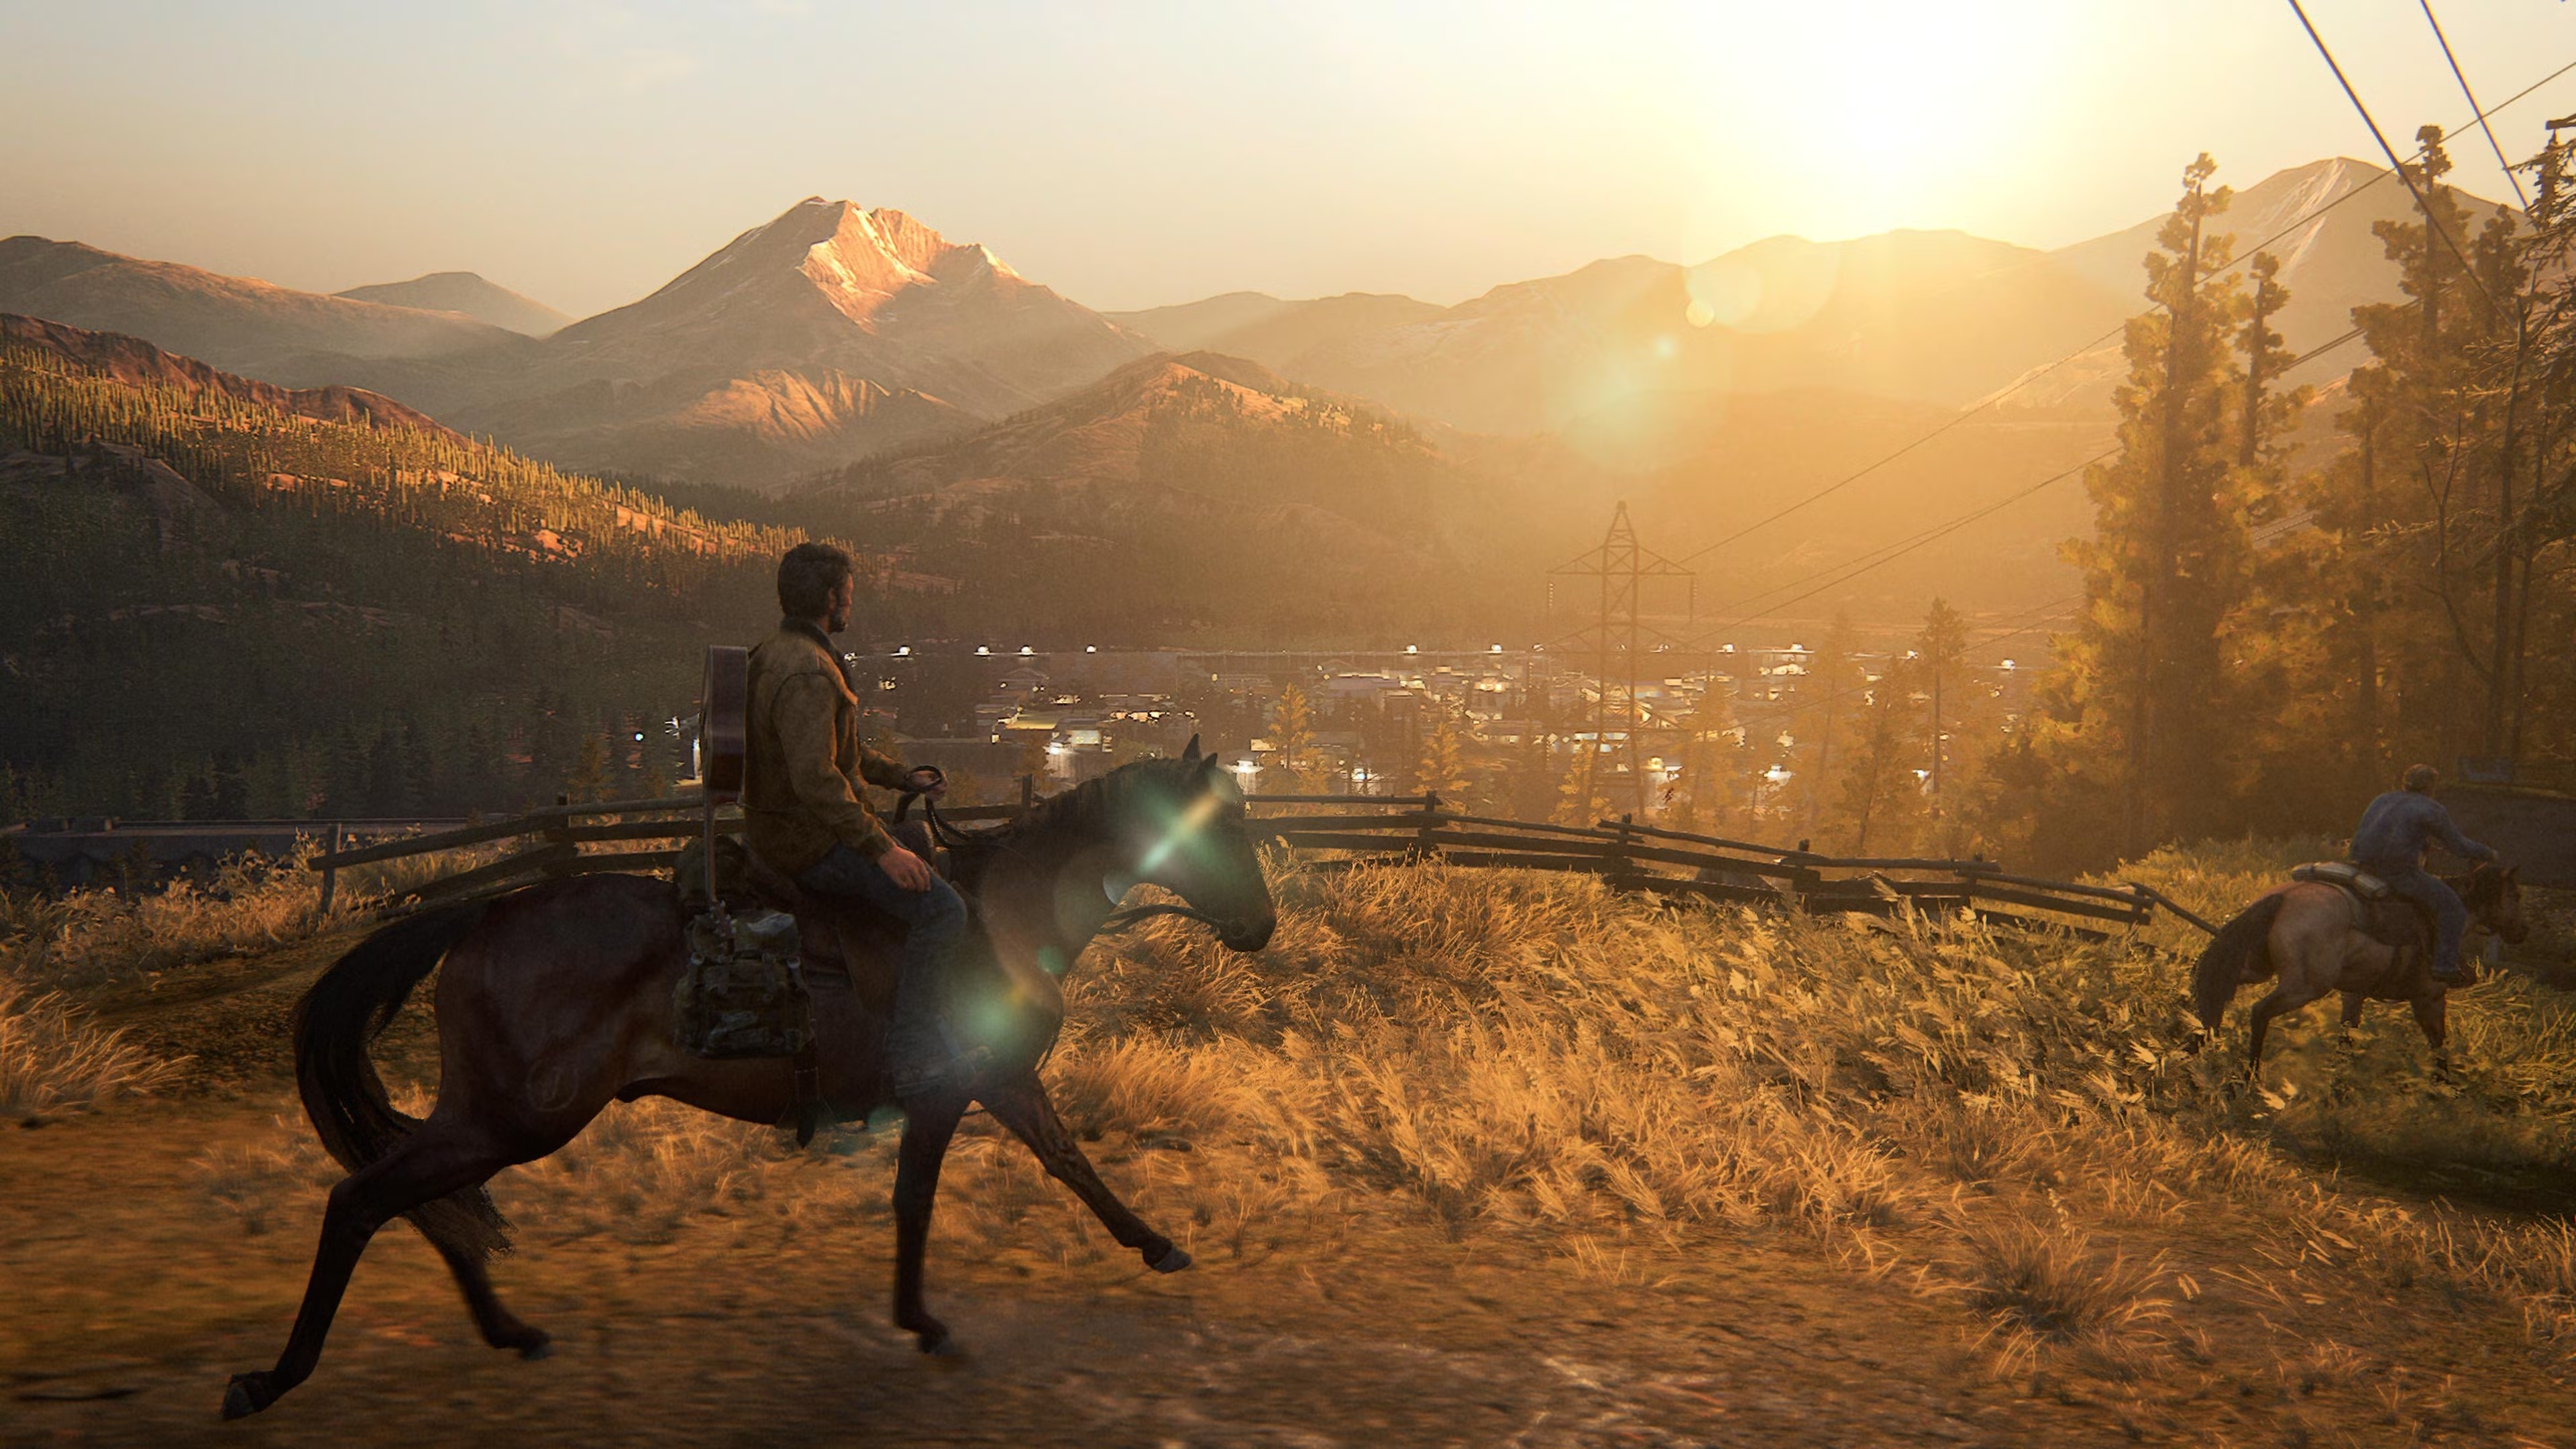
\includegraphics[width=1\linewidth]{imagenes/tlou2.jpg}
	\caption[\textbf{Captura de The Last of Us Parte II}.]{\textbf{Captura de The Last of Us Parte II}, elegido Juego del Año 2020 por los principales medios de la industria. Este videojuego alcanza un nivel gráfico y narrativo sobresaliente. \href{https://static1.srcdn.com/wordpress/wp-content/uploads/2024/01/tlou2r-joel-horse.JPG}{https://static1.srcdn.com/wordpress/wp-content/uploads/2024/01/tlou2r-joel-horse.JPG}}
	\label{foto-the-last-of-us-2}
\end{figure}

También, gracias a la emulación de consolas clásicas, las ofertas diarias, los videojuegos gratuitos, los títulos free-to-play y los servicios de suscripción como Game Pass o PS Plus, es posible acceder a una gran variedad de videojuegos de forma gratuita o a un precio reducido.  


No obstante, el aumento en los costos y recursos necesarios para desarrollar un videojuego \textit{triple A} (término que hace referencia a títulos de gran producción, con una alta inversión en desarrollo y publicidad) ha provocado que los lanzamientos de las sagas más conocidas se espacien cada vez más. Ejemplos de ello son el esperado \textit{Grand Theft Auto VI}, que ha tardado 12 años en llegar desde el lanzamiento de \textit{Grand Theft Auto V}, y \textit{The Elder Scrolls VI}, cuya espera alcanza los más de 14 años desde \textit{The Elder Scrolls V}, según la fecha de realización de este trabajo.  


Debido a esta situación, si queremos disfrutar de experiencias similares a nuestros videojuegos favoritos, a menudo debemos recurrir a entregas anteriores de la misma saga que no jugamos en su momento o bien buscar alternativas en títulos de características similares.  


Algunas plataformas actuales, como Xbox o Steam, recomiendan videojuegos en función de nuestras compras, de los títulos que se han jugado recientemente o de manera aleatoria. Sin embargo, estas recomendaciones no tienen en cuenta factores importantes, como los recursos de los que disponemos en ese momento, la accesibilidad, el deseo de cambiar de género de videojuego o la disponibilidad de otra plataforma, entre otros.  


Ante esta necesidad, se propone una solución basada en una plataforma capaz de tener en cuenta todos estos factores de manera automatizada, con el objetivo de ofrecer recomendaciones personalizadas según las características y preferencias del usuario.



Parecería que contemplar todos los géneros de videojuegos, sus características y las distintas plataformas es una tarea ardua. No obstante, gracias al avance de la tecnología, contamos con modelos generativos de lenguajes que han sido entrenados con millones de datos, incluidos videojuegos.  

Si aprovechamos esta tecnología a nuestro favor, podemos obtener fácilmente recomendaciones en tiempo real según los requisitos especificados, utilizando información de consultas previas e incluso teniendo en cuenta los videojuegos que poseemos en nuestra biblioteca, gracias a la vinculación de plataformas de videojuegos con nuestra propia plataforma.  


Los avances recientes en inteligencia artificial han permitido el desarrollo de modelos generativos de lenguaje entrenados con grandes cantidades de datos, incluidos videojuegos, lo que abre nuevas posibilidades para crear recomendaciones más inteligentes y contextuales.


A lo largo de este trabajo, se explorarán distintas tecnologías relacionadas con el procesamiento del lenguaje natural y su aplicación en sistemas de recomendación, con el fin de desarrollar una plataforma eficiente, escalable e intuitiva.



El resto del documento se estructura de la siguiente manera:

\begin{itemize}
	\item \textbf{Capítulo 2}: Se explica qué son los modelos generativos de lenguaje y en qué consiste LangChain, además de analizar algunos trabajos previamente realizados.
	
	\item \textbf{Capítulo 3}: Se presentan los objetivos del proyecto, así como la planificación temporal y el presupuesto estimado.
	
	\item \textbf{Capítulo 4}: Se analizan los distintos requisitos de la aplicación, explicando también el proceso seguido para su obtención.
	
	\item \textbf{Capítulo 5}: Se describe la arquitectura general del sistema, detallando los diferentes componentes que lo conforman y su interacción.
	
	\item \textbf{Capítulo 6}: Se explica la implementación de la plataforma, incluyendo las tecnologías utilizadas, el desarrollo de cada módulo y el procedimiento para su ejecución.
	
	\item \textbf{Capítulo 7}: Se recogen las pruebas realizadas para verificar y validar el correcto funcionamiento de la aplicación.
	
	\item \textbf{Capítulo 8}: Se exponen las conclusiones obtenidas a lo largo del desarrollo del trabajo, así como posibles líneas futuras de mejora o ampliación.
\end{itemize}







 
\clearpage \thispagestyle{empty} \null \clearpage

\chapter{Contexto y estado del arte }

En este capítulo se especificarán las tecnologías que se utilizarán en el proyecto. Describiremos en qué consisten, qué nos ofrecen y cómo se aplican específicamente al desarrollo de esta plataforma. 

Además, revisaremos otros trabajos realizados que empleen estas tecnologías, con un enfoque particular en \textit{LangChain}, que constituye el pilar fundamental de este proyecto.  

\newpage

\section{Contexto}

\subsection{Procesadores de lenguajes}

Un \textbf{procesador de lenguaje} es un software diseñado para entender, analizar, interpretar y generar lenguaje humano mediante un ordenador. Estos sistemas permiten a las máquinas interactuar con los seres humanos de una manera más natural, utilizando los lenguajes que empleamos en la vida cotidiana. Para lograr este objetivo, los procesadores de lenguaje se basan en modelos de aprendizaje automático que, en términos generales, crean estructuras computacionales capaces de aprender patrones y estructuras lingüísticas a partir de grandes volúmenes de datos provenientes de diversos ámbitos, incluidos los videojuegos.

El desarrollo de un procesador de lenguaje sigue un proceso estructurado que incluye varias etapas. En primer lugar, se diseñan modelos matemáticos y algoritmos que permiten a las máquinas "comprender" la estructura y la semántica del lenguaje. A continuación, estos modelos se entrenan utilizando millones de datos lingüísticos, como textos, conversaciones y otras fuentes, lo que les permite adquirir la capacidad de realizar tareas complejas, como la traducción o la generación de texto en respuesta a preguntas o peticiones específicas.

Algunos de los procesadores de lenguaje más avanzados en la actualidad son \textbf{ChatGPT}, desarrollado por OpenAI, y \textbf{Gemini}, creado por Google. Ambos sistemas emplean tecnologías basadas en redes neuronales profundas y han alcanzado un nivel de sofisticación que les permite realizar tareas complejas, como la redacción de textos, la resolución de problemas y la generación de contenido con una precisión similar a la de un experto en la materia.

Gracias a su capacidad de comprensión, conocimiento y razonamiento, un uso adecuado de estos sistemas puede generar recomendaciones precisas en prácticamente cualquier ámbito. En nuestro caso, el sector de los videojuegos se beneficia enormemente, ya que existe una gran cantidad de información en la red, que es utilizada en el entrenamiento de muchos modelos. Existen miles de análisis de videojuegos que los clasifican según su género, plataforma, calidad y otros criterios. Además, hay información relevante sobre requisitos técnicos, títulos similares o la mejor plataforma para jugar cada juego. Buscar esta información de manera manual puede ser complicado, ya que no siempre conocemos las mejores fuentes de análisis o los idiomas en los que están disponibles. Sin embargo, los procesadores de lenguaje han sido entrenados con esta información y pueden proporcionarnos respuestas de manera sencilla, interactiva e incluso interpretando nuestras intenciones implícitas.

En resumen, los procesadores de lenguaje no solo están diseñados para facilitar la comunicación entre humanos y máquinas, sino que también están transformando la manera en que interactuamos con la tecnología. En este proyecto, desempeñarán un papel fundamental en la generación de recomendaciones personalizadas de videojuegos.

\begin{figure}[H]
    \centering
    
\includegraphics[width=1\linewidth]{imagenes/pdl.jpg}
    \caption[\textbf{Ejemplos de procesadores de lenguaje}.]{\textbf{Ejemplos de procesadores de lenguaje}. ChatGPT, Gemini y Copilot, tres de los procesadores de lenguaje más avanzados y reconocidos en la actualidad. \href{https://static1.srcdn.com/wordpress/wp-content/uploads/2024/01/tlou2r-joel-horse.JPG}{https://static1.srcdn.com/wordpress/wp-content/uploads/2024/01/tlou2r-joel-horse.JPG}}
    \label{procesadores-de-lenguaje}
\end{figure}

\newpage

\subsection{LangChain}

Para comprender mejor esta tecnología, obtendremos la información  de su página web oficial.

LangChain es una tecnología que permite a las aplicaciones razonar y procesar información de manera más inteligente. Es utilizada por múltiples empresas de gran renombre, como Google y Rakuten TV. LangChain facilita la construcción de aplicaciones que integran procesadores de lenguaje, permitiendo que estas interactúen de forma dinámica y contextual con los usuarios.

Para cadenas y flujos de recuperación más sencillos, se recomienda usar LangChain junto con LangChain Expression Language para ensamblar componentes. Si estamos creando agentes o necesitamos una orquestación más compleja, utilizamos LangGraph.

Por otro lado, \textbf{LangGraph Platform} se encarga de la ejecución, permitiendo desplegar y ejecutar las aplicaciones de manera eficiente. Además, \textbf{LangSmith} ofrece herramientas para gestionar y probar las aplicaciones, asegurando su correcto funcionamiento y mejorando el rendimiento. \cite{PaginaLangChainOficial}



\begin{figure}[H]
    \centering
    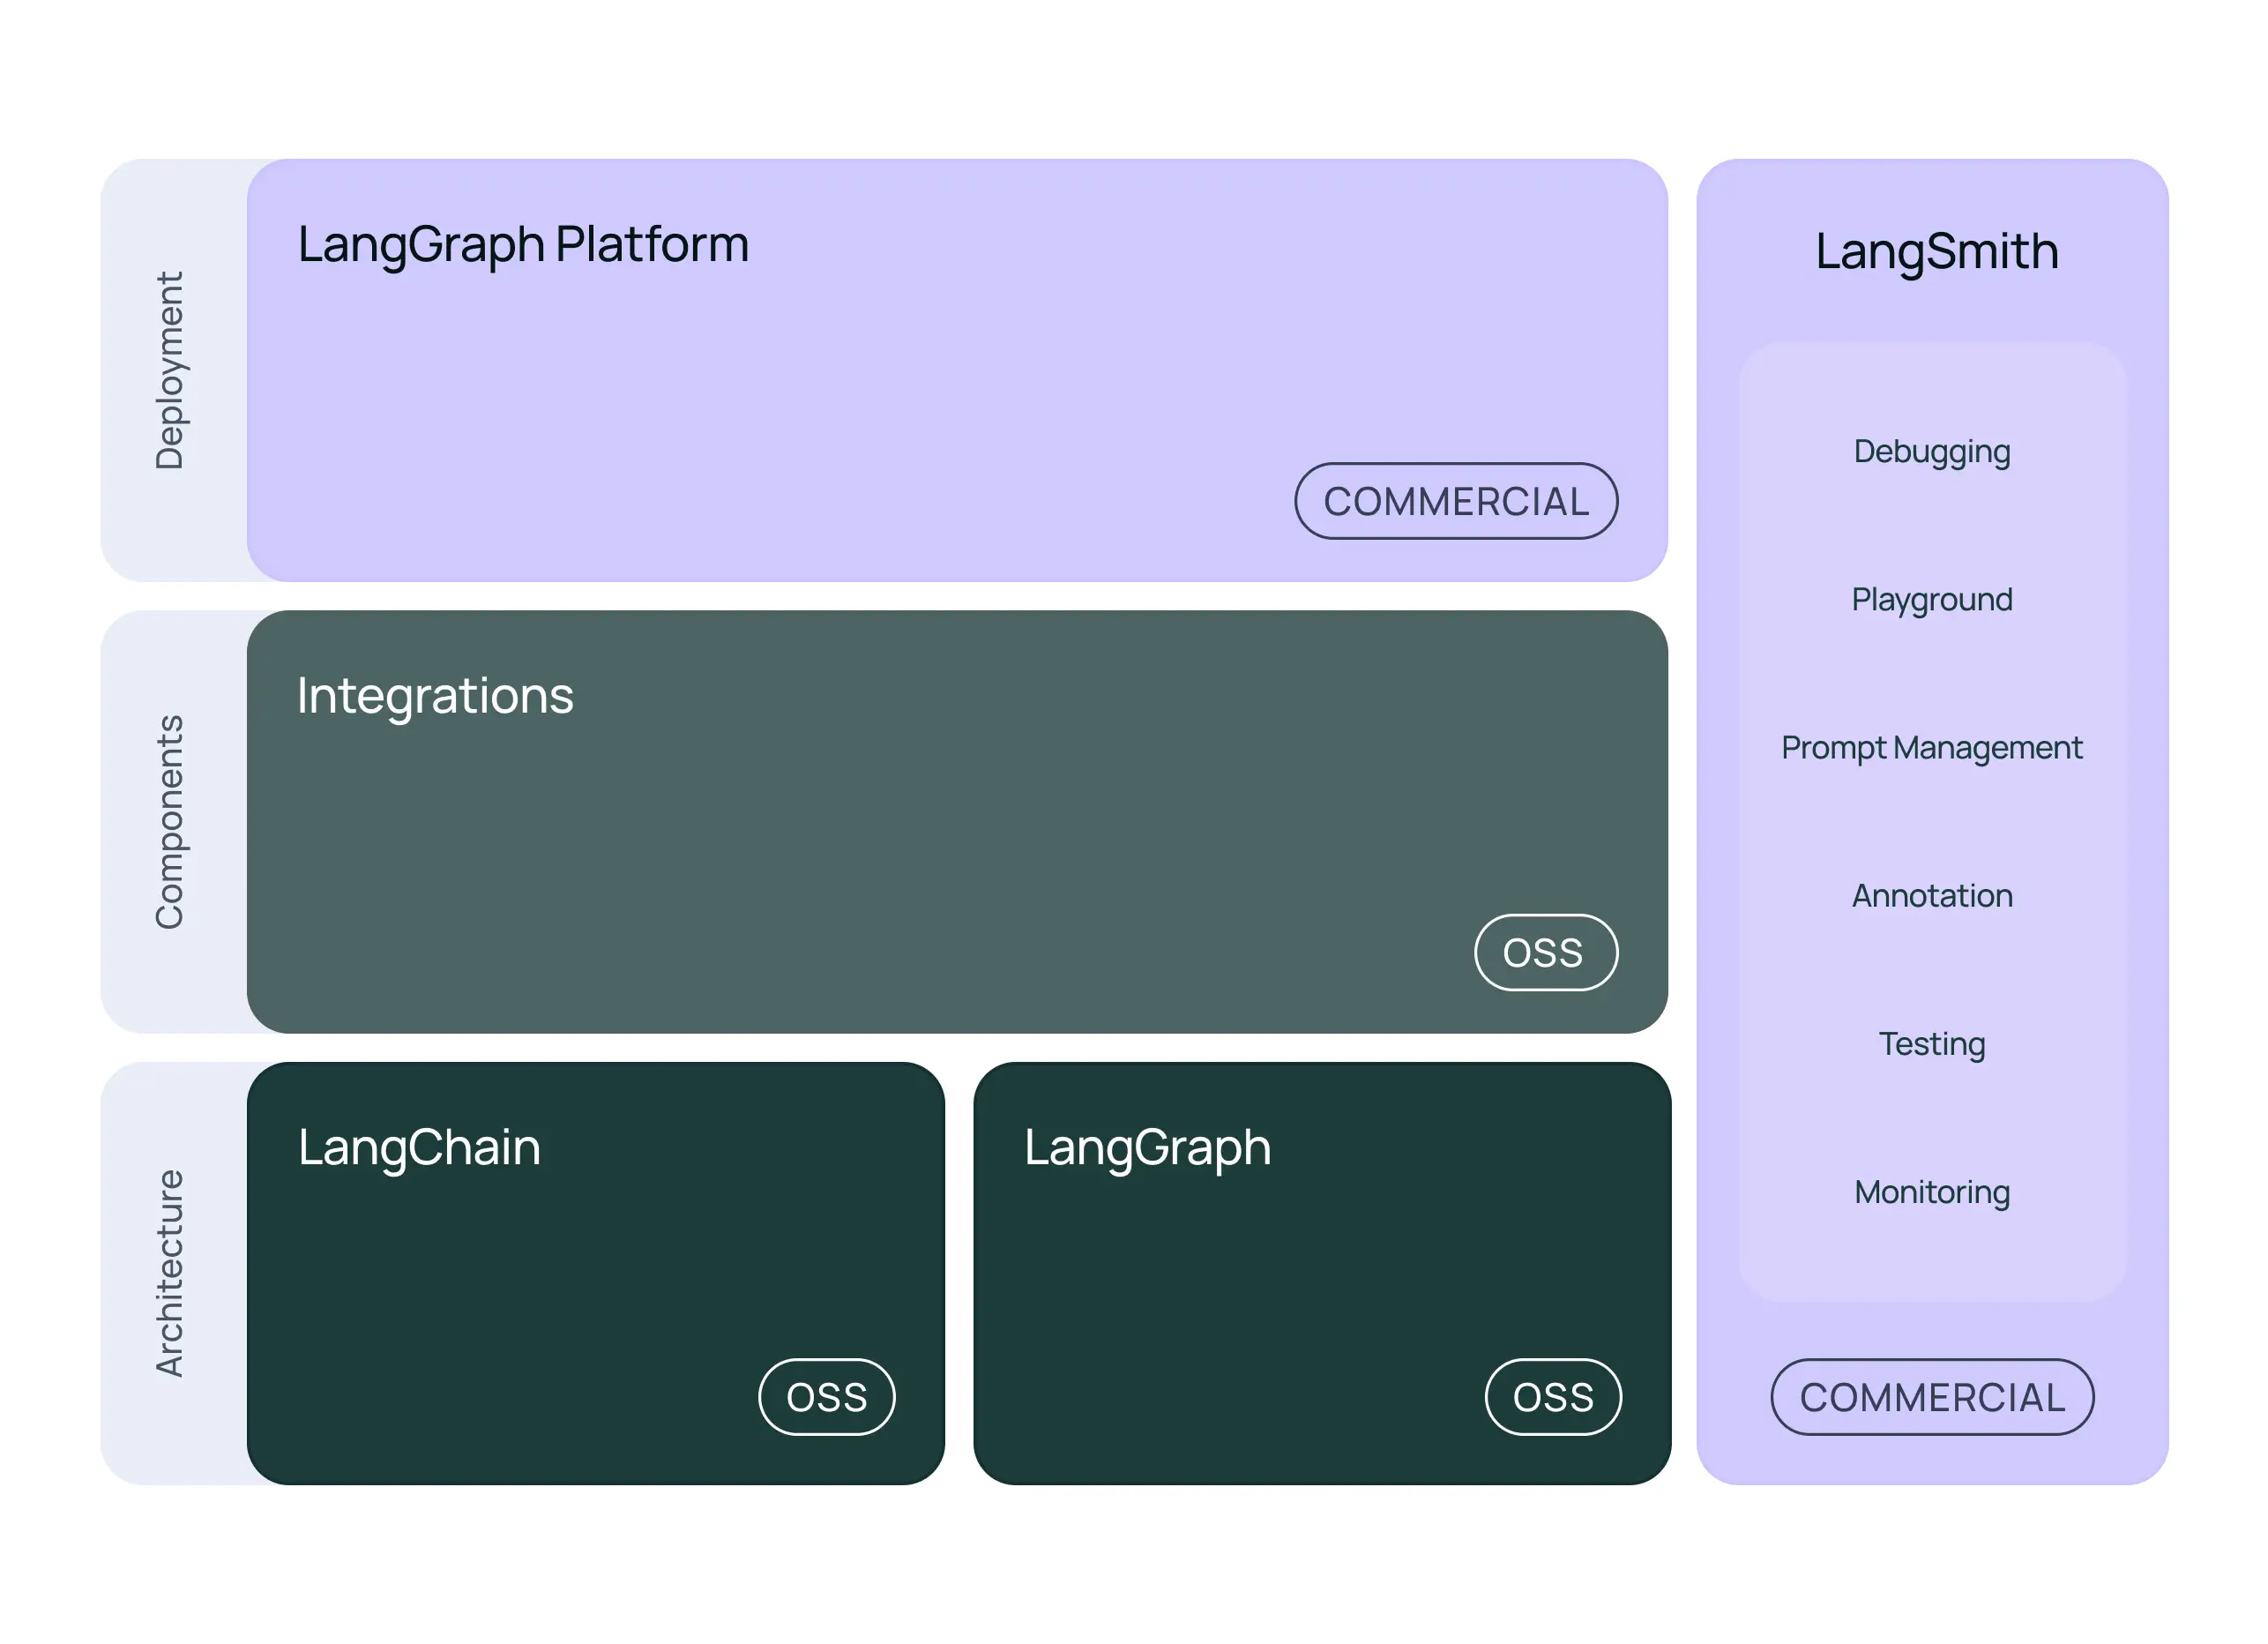
\includegraphics[width=\linewidth]{imagenes/lg.jpg}
    \caption[\textbf{Arquitectura productos LangChain}.]{\textbf{Arquitectura productos LangChain}. La arquitectura de referencia que las empresas adoptan para el éxito. Los productos de LangChain pueden usarse de forma independiente o combinada para lograr un impacto multiplicador, guiando en la construcción, ejecución y gestión de aplicaciones LLM. \cite{PaginaLangChainOficial}}
    \label{productos-lang-chain}
\end{figure}


Procedamos a analizar cada producto por separado.


\subsubsection{LangChain básico}

Es la tecnología base de todos los productos. Es compatible con JavaScript y Python. Cuenta con una amplia biblioteca de componentes para usar de principio a fin en las aplicaciones. Conecta los procesadores de lenguaje con cualquier fuente de datos o conocimiento, y APIs para crear aplicaciones conscientes del contexto y con capacidad de razonamiento, utilizando métodos populares como RAG (Retrieval-Augmented Generation), que recupera la información del usuario de, por ejemplo, bases de datos antes de generar una respuesta, para mejorarla; y cadenas simples, en las que se solicita la pregunta al usuario, se pasa al procesador de lenguaje y se envía la respuesta al usuario. LangChain es fácil de comenzar a usar y ofrece elección, flexibilidad y potencia a medida que escalas. Cuenta con más de 3000 colaboradores, la comunidad más grande de cualquier framework centrado en LLM, más de 600 integraciones y es fácil de usar, pero robusto para producción. Además, es de código abierto. \cite{PaginaLangChainOficialBasico}


\subsubsection{Métodos}

En LangChain, diversos métodos avanzados permiten optimizar la interacción con los procesadores de lenguaje, facilitando la integración de datos, la mejora en el procesamiento y la generación de respuestas. Estos métodos permiten adaptar el comportamiento del sistema a necesidades específicas, desde la recuperación de información relevante hasta la ejecución de tareas automatizadas mediante agentes. Vamos a explorar algunos de los métodos clave utilizados en LangChain, como la Generación Aumentada por Recuperación (RAG), los agentes inteligentes y las herramientas de evaluación de rendimiento, que son fundamentales para el desarrollo de aplicaciones inteligentes y contextualmente conscientes.

\textbf{RAG}

La \textbf{Generación Aumentada por Recuperación (RAG)} con LangChain y sus métodos integrados de gestión y recuperación conecta los datos con el poder de los procesadores de lenguaje. Dispone de herramientas de importación de documentos para cualquier tipo de datos.

Cuenta con potentes algoritmos de recuperación como:

\begin{itemize}
    \item \textbf{Time-Weighted Vector Store:} combina la similitud semántica con un decaimiento temporal para tener en cuenta la actualidad en las recuperaciones.
    \item \textbf{Parent Document Retriever:} incorpora fragmentos pequeños, que son mejores para la búsqueda por similitud, pero recupera fragmentos más grandes que ayudan en la generación de contenido.
    \item \textbf{Self Query Retriever:} analiza la consulta en lenguaje natural y escribe una consulta estructurada para ejecutarla en el VectorStore subyacente.
    \item \textbf{Contextual Compression:} comprime el documento recuperado utilizando el contexto de la consulta, de modo que solo se devuelve la información relevante de la fuente.
    \item \textbf{Multi Vector Retriever:} realiza consultas en múltiples vectores almacenados por documento, incluidos fragmentos más pequeños, resúmenes y preguntas hipotéticas.
\end{itemize}

La API de indexación de LangChain sincroniza los datos desde cualquier fuente hacia un almacén vectorial, ayudándote a ahorrar tiempo y recursos. \cite{PaginaLangChainOficialRAG}

\textbf{Agentes}

Los agentes pueden crear borradores iniciales para revisión a posteriori, actuar en tu nombre o esperar tu aprobación antes de la ejecución. LangGraph ofrece control para flujos de trabajo personalizados de agentes y multi-agentes, interacciones fluidas con intervención humana, y soporte nativo para transmisión de datos, lo que mejora la fiabilidad y ejecución de los agentes. Permite llamar de manera forzada a una herramienta, esperar la aprobación de intervención humana, la colaboración de múltiples agentes en un objetivo común y transmitir los pasos intermedios a medida que ocurren. Además, LangSmith ofrece la capacidad de explicar por qué los agentes se desvían y cómo hacer que vuelvan a funcionar correctamente. \cite{PaginaLangChainOficialAgentes}

\textbf{Evaluación}

LangSmith permite medir el rendimiento de la aplicación a lo largo de todo su ciclo de desarrollo con multitud de métricas. Se puede usar evaluación offline, con integración continua y online.

Un marco de pruebas sólido comienza con la creación de un conjunto de datos de referencia, una tarea que a menudo resulta tediosa. LangSmith simplifica esto permitiéndote guardar las trazas de depuración y producción en conjuntos de datos. Los conjuntos de datos son colecciones de entradas y salidas ejemplares o problemáticas que deben ser replicadas o corregidas, respectivamente. También te permite hacer un seguimiento de cómo se comparan las diferentes versiones de tu aplicación según los criterios de evaluación que hayas definido. Además, facilita la evaluación humana y en línea, no solo latencia, errores y costos, sino también medidas cualitativas para asegurar que tu aplicación responda de manera efectiva y cumpla con las expectativas del usuario. \cite{PaginaLangChainOficialEvaluacion}


 
\subsubsection{LangGraph}

LangGraph controla, modera y guía las acciones de los agentes, evitando que se desvíen del curso previsto. Permite diseñar flujos de control diversos, tales como simples, multi-agentes, jerárquicos o secuenciales, todo dentro de un único marco de trabajo. Además, tiene la capacidad de guardar los historiales de conversación y los datos de la sesión, lo que permite mantener el contexto a lo largo del tiempo y asegurar transferencias suaves de información, incluso hacia atrás.

LangGraph ofrece múltiples opciones de despliegue, incluye un estudio visual y es de código abierto, lo que facilita su integración y personalización.

Asimismo, cuenta con una plataforma diseñada para desplegar y escalar aplicaciones LangGraph, con una API orientada a la creación de interfaces de usuario (UX) para agentes, además de un entorno de desarrollo integrado. Sin embargo, a diferencia de su núcleo, esta plataforma no es de código abierto.\cite{PaginaLangChainOficialLangGraph}


 

\subsubsection{LangSmith}

LangSmith es una plataforma todo en uno diseñada para desarrolladores, que abarca cada etapa del ciclo de vida de las aplicaciones impulsadas por procesadores de lenguaje, tanto si utilizan LangChain como si no.

Esta herramienta permite depurar, colaborar, realizar pruebas y monitorear, ofreciendo una visibilidad completa de toda la secuencia de llamadas. Esto facilita la identificación precisa de errores y cuellos de botella en el rendimiento en tiempo real. Además, permite revisar, etiquetar y evaluar el comportamiento de los agentes de forma sencilla, mejorando así la eficiencia y la fiabilidad del sistema.  

LangSmith también puede ejecutarse de forma local, proporcionando flexibilidad y control total sobre el entorno de desarrollo.  \cite{PaginaLangChainOficialLangSmith}

\newpage
\section{Estado del arte}

La revisión de la literatura existente nos permite comprobar si ya se ha desarrollado un proyecto similar al nuestro, lo que puede servir como fuente de inspiración, guía o referencia para evaluar la novedad de nuestro trabajo.

Tras una exhaustiva búsqueda, no se ha encontrado ningún trabajo o artículo que aborde específicamente el uso de LangChain para la recomendación de videojuegos. Esto sugiere que nuestro proyecto podría ser innovador en este ámbito.

Sin embargo, en una búsqueda más general, se han identificado artículos relacionados que merecen ser destacados:

Un caso relevante es el de las \textbf{recomendaciones} en otros ámbitos \textbf{utilizando LangChain}. En un trabajo publicado por el Journal of Industrial Engineering and Applied Science, se observa cómo un grupo de estudiantes diseñó un sistema para recomendar anime de manera personalizada, utilizando LangChain. Los resultados obtenidos sometidos a numerosas métricas fueron muy satisfactorios gracias a las capacidades de esta tecnología. \cite{LangChainAnime}

Otro trabajo notable es el de Johans Quintero, quien desarrolló un sistema que recomienda recursos mediante mecanismos de Procesamiento de Lenguaje Natural, utilizando agentes de LangChain. Este proyecto se centra principalmente en la recomendación de libros, pero su enfoque podría extrapolarse a otros ámbitos. \cite{recommender-agent-langchain}

En cuanto a la \textbf{recomendación de videojuegos}, se han encontrado trabajos relevantes que utilizan otras tecnologías. Por ejemplo, Daniel Yélamos Pérez creó un sistema de recomendación de videojuegos basado en las opiniones de otros usuarios, empleando técnicas de extracción e interpretación semántica de datos en un entorno informal. \cite{recomendacion-videojuegos-uam}

Por último, cabe mencionar el trabajo de Alejandro Roldán Soblechero, quien desarrolló una aplicación móvil que permite a los usuarios opinar sobre videojuegos. Esta aplicación integra datos de IGDB (Internet Game Database) y otras bases de conocimiento, garantizando la solidez y actualidad de las sugerencias generadas por el sistema de recomendación. \cite{aplicacion-recomendacion-uoc}


Estos estudios evidencian que tanto el ámbito de las recomendaciones de videojuegos como el uso de LangChain en sistemas de recomendación son temas explorados en la literatura, ofreciendo un valioso punto de referencia y posibles fuentes de inspiración. Sin embargo, la ausencia de trabajos que combinen específicamente LangChain con la recomendación de videojuegos destaca la originalidad y el carácter innovador de nuestro proyecto. 
\clearpage \thispagestyle{empty} \null \clearpage
\chapter{Objetivos y metodología de desarrollo}

En este capítulo se define el objetivo principal del proyecto, junto con los objetivos específicos que permitirán alcanzarlo de manera efectiva.

Asimismo, se detallará la metodología de trabajo utilizada en el desarrollo de la plataforma, describiendo los enfoques y herramientas empleados en el desarrollo para este trabajo.
\newpage
\section{Objetivos}

Para alcanzar una meta, es fundamental definir con precisión qué se desea lograr y establecer los pasos y condiciones necesarios para lograrlo de manera efectiva.

El \textbf{objetivo principal} de este trabajo es \textbf{desarrollar un sistema de recomendación de videojuegos} que ofrezca sugerencias personalizadas y alineadas con las preferencias y necesidades del usuario.

Para alcanzar este objetivo de manera óptima, es esencial cumplir con los siguientes objetivos secundarios:

\begin{itemize}
    \item \textbf{Diseñar una interfaz clara, intuitiva y accesible} para garantizar una experiencia de usuario fluida y sin barreras.
    \item \textbf{Mejorar la personalización del sistema} mediante el aprendizaje y almacenamiento de las interacciones del usuario, así como la integración de datos provenientes de otras plataformas.
    \item \textbf{Implementar y coordinar múltiples modelos de lenguaje} para optimizar la precisión y diversidad de las recomendaciones.
    \item \textbf{Incorporar factores adicionales en las recomendaciones}, como disponibilidad del juego, requisitos técnicos, accesibilidad y presupuesto del usuario.
    \item \textbf{Facilitar la actualización del sistema} con nuevas tendencias y lanzamientos en el sector de los videojuegos, considerando las limitaciones en el entrenamiento de los modelos de lenguaje.
    \item \textbf{Optimizar el rendimiento del sistema} para ofrecer respuestas rápidas, precisas y justificadas, mejorando la experiencia de usuario.
    \item \textbf{Garantizar la privacidad y seguridad de los datos} mediante buenas prácticas de almacenamiento y procesamiento de información.
\end{itemize}

El cumplimiento de estos objetivos asegurará el desarrollo de un sistema de recomendación eficaz y adaptado a las necesidades del usuario.
\newpage
\section{Metodología de desarrollo}

Para el \textbf{desarrollo} de la plataforma, se ha adoptado un enfoque basado en \textbf{metodologías ágiles}, priorizando la \textbf{flexibilidad} y la \textbf{adaptación} continua a los desafíos y necesidades emergentes a lo largo del proceso. Las metodologías ágiles se centran en la entrega \textbf{incremental} de valor, permitiendo \textbf{ajustes rápidos y frecuentes} en función de los comentarios, necesidades e inconvenientes surgidos a lo largo del desarrollo. Este enfoque se caracteriza por ciclos de trabajo cortos, denominados "\textbf{sprints}", en los cuales se planifica, ejecuta, prueba y evalúa el progreso de manera continua, asegurando la flexibilidad y la rápida implementación de cambios.

La \textbf{planificación} inicial fue un proceso caótico. Aunque comencé con una idea general del proyecto, a medida que avanzaba, fui desarrollando cada sección de la memoria de forma paralela, sin perder de vista cómo se conectaban entre sí los capítulos y cómo se iban integrando los distintos elementos del trabajo. La planificación fue en constante evolución, adaptándose a los tiempos limitados y a los factores externos imprevistos, lo que permitió cumplir con los objetivos, aunque de manera más flexible y con ajustes frecuentes en el camino.

A medida que el desarrollo fue avanzando, la planificación se fue optimizando mediante el establecimiento de objetivos más concretos y plazos más definidos para cada sprint. De esta manera, se lograron entregas parciales de la plataforma, que permitieron validar la funcionalidad y realizar mejoras progresivas en cada ciclo. Además, la iteración continua y la retroalimentación temprana de las soluciones implementadas ayudaron a reducir riesgos y garantizar la calidad del producto final.

La planificación se podría resumir en esta diagrama de Gantt:

\begin{figure}[H]
	\centering
	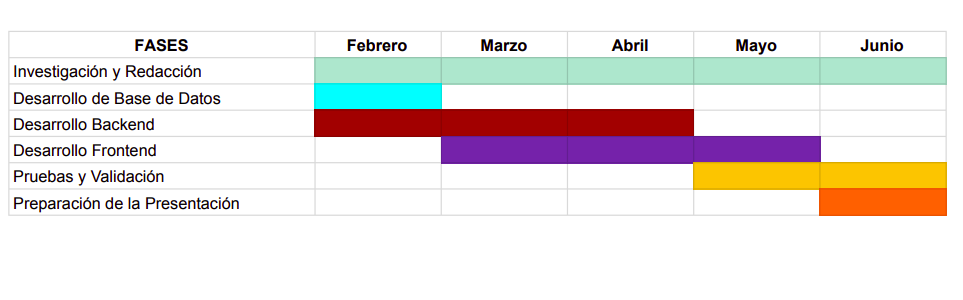
\includegraphics[width=1\linewidth]{imagenes/diagrama.png}
	\caption[\textbf{Planificación en diagrama de Gantt}.]{\textbf{Planificación en diagrama de Gantt}. Apreciamos como el proyecto se ha realizado a través de los meses. La memoria y la investigación son apartados que evolucionan continuamente. Los distintos elementos de la aplicación se desarrollan por partes, pero en ciertos puntos se integran de forma paralela. Las prueba y presentación se realiza al final, pero durante todo el proceso se tiene en mente.}
	\label{diagrama}
\end{figure}

Sin embargo, es importante volver a señalar que, debido a mis circunstancias personales, no pude dedicarle mucho tiempo a la organización temporal del proyecto. En mi caso, la gestión del tiempo no ha sido un aspecto en el que pudiera destacar, ni en este trabajo ni en otros aspectos de toda mi vida. Por lo tanto, preferí concentrarme en lo verdaderamente importante: la realización efectiva del trabajo, sin gastar tiempo innecesario en crear planificaciones detalladas solo para cumplir con una formalidad. La prioridad fue avanzar en el desarrollo y en los resultados concretos, adaptándome a lo que surgiera en el camino. \textit{\textbf{Carpe Diem}}.


La \textbf{investigación} ha sido fundamental en la metodología de trabajo, recurriendo a documentación oficial, artículos técnicos y foros especializados para resolver dudas y optimizar la implementación. Además, se adoptó un enfoque práctico basado en la experimentación, probando diversas soluciones y herramientas para garantizar el correcto funcionamiento de la plataforma y su integración.

El uso de herramientas como \textit{ChatGPT} facilitó la corrección ortográfica, la mejora de la redacción y la traducción de textos en otros idiomas, acelerando así el proceso de adquisición de conocimiento y optimizando el tiempo dedicado a la investigación.

\subsection{Presupuesto}

Dado que el proyecto se ha desarrollado de manera autónoma y sin recursos financieros dedicados, los \textbf{costes} asociados se limitan al tiempo invertido, el uso de mis recursos propios, como ordenador y wifi, y al uso de herramientas gratuitas. A continuación, se detalla el presupuesto estimado basado en los costes de un desarrollador informático y los recursos utilizados que podría adecuarse a una empresa:

\begin{itemize}
    \item \textbf{Coste del desarrollador informático:} Según los estándares actuales, el coste medio por hora de un informático en España para un trabajo de este tipo es de aproximadamente 15,27€ por hora\cite{sueldo}. Dado que un TFG dura 300 horas, el cálculo sería el siguiente:
    \[
    300 \, \text{horas} \times 15,27 \, \text{€} = 4.581 \, \text{€}
    \]
    Este coste es aproximado y puede variar dependiendo de la experiencia y la localización del profesional.

    \item \textbf{Equipo informático:} El coste estimado de un ordenador adecuado para el desarrollo de software es de aproximadamente 1.420€, más un ratón de unos 26 €, considerando un equipo de gama media-alta, como es mi caso. Aunque como este desarrollo no requiere de una GPU de alta prestaciones, ya que no se genera casi gráficos ni se hacen muchos cálculos, es perfectamente viable usar un equipo más barato que no tenga una GPU dedicada, o que esta sea una básica destinada a la ofimática.

    \item \textbf{Consumo de electricidad:} El consumo de un ordenador durante un período de 300 horas puede suponer un coste de aproximadamente 42€ (suponiendo un consumo medio de 0.2 kWh(portátil enchufado más una lámpara) por hora\cite{luz} y un coste de unos 0.14€ por kWh). El coste de la electricidad es un factor muy importante a tener en cuenta. Aunque se ha estimado un gasto general, es necesario señalar que este costo puede ser en realidad mayor debido a las tarifas diferenciadas por franjas horarias, las cuales, lamentablemente, están bastante elevadas en las franjas activas. Esta situación resulta aún más agravante al considerar el aumento constante de los precios de la energía, lo que incrementa considerablemente los costes operativos de los proyectos que requieren un uso constante de equipos eléctricos. Es incluso más vergonzoso ver cómo la precariedad de nuestros dirigentes —más interesados en montar un circo entre ellos que en hacer las cosas bien y con responsabilidad— nos deja sin luz casi un día entero, costándonos a muchos una valiosa jornada de trabajo, e incluso, en algunos casos, algo aún peor: la vida. Es lamentable comprobar cómo no hay consecuencias para los culpables, sino aplausos de sus fieles, sumisos como ganado.


    \item \textbf{Conexión a internet:} El coste de un servicio básico de internet(sin contar las líneas móviles) es de alrededor de 30€ con MasMovil. Suponiendo que el proyecto dure 6 meses, el coste estimado de la conexión a internet sería:
    \[
    30 \, \text{€} \times 6 \, \text{meses} = 180 \, \text{€}
    \]

    \item \textbf{Herramientas y servicios en línea:} Las herramientas utilizadas, como \textit{GitHub}, \textit{LangChain}, \textit{LangGraph} y \textit{ChatGPT}, fueron utilizadas en sus versiones gratuitas, lo que ha permitido minimizar los costes. No obstante, en un entorno profesional, estos servicios pueden tener un coste mensual que suele variar entre 10€ y 100€ dependiendo de las funcionalidades requeridas.

    \item \textbf{Juego en Steam:} Steam requiere un gasto directo de al menos 5 dólares para habilitar ciertas funciones, como la lista de amigos, actividades o el acceso a sus APIs. En mi caso, no había alcanzado ese umbral, ya que suelo adquirir juegos mediante plataformas de keys, que generalmente ofrecen mejores precios y no dependen de los periodos de rebajas oficiales de Steam. Compré Cult of the Lamb por 11,49€, lo que activó esas funcionalidades.
    
\end{itemize}

\textbf{Resumen del presupuesto estimado:}

\begin{itemize}
    \item \textbf{Coste del desarrollador informático:} 4.581€
    \item \textbf{Equipo informático:} 1.446€ (incluyendo ratón)
    \item \textbf{Consumo de electricidad:} 42€
    \item \textbf{Conexión a internet:} 180€
    \item \textbf{Herramientas en línea (versión gratuita):} 0€
    \item \textbf{Juego de Steam:} 11.49€
\end{itemize}

\textbf{Total estimado de costes (sin incluir costes de servicios pagos):} 6.260.49€

Este presupuesto refleja el coste real de desarrollar el proyecto de manera autónoma, sin considerar gastos adicionales relacionados con licencias de software, servicios profesionales o materiales externos.

\textbf{Conclusión}


La metodología ágil permitió una planificación flexible y adaptable a los retos del proyecto, lo que garantizó el éxito del desarrollo de la plataforma. Además, el uso de herramientas gratuitas y la optimización de recursos han permitido mantener los costes del proyecto en niveles razonables, asegurando que el objetivo final se alcanzara dentro de los plazos establecidos, sin comprometer la calidad del trabajo realizado.



\clearpage \thispagestyle{empty} \null \clearpage
\chapter{Análisis}

En este capítulo se analizarán en detalle los requisitos de la plataforma, abarcando tanto los requisitos funcionales como los no funcionales y los de información. También se describirán los casos de uso. Se examinarán las necesidades del usuario y las características esenciales del sistema.

Además, se abordará el proceso de obtención de requisitos.

Este análisis servirá como base para la fase de diseño y desarrollo, garantizando que la plataforma cumpla con los objetivos definidos y proporcione una experiencia óptima para los usuarios.

\newpage
\section{Obtención de Requisitos}

La definición de los requisitos del sistema se ha basado en mi extensa experiencia en el sector de los videojuegos, combinada con la retroalimentación de amigos y jugadores con los que he interactuado a lo largo de los años. Además, he tenido la oportunidad de observar y analizar constantemente el panorama del mundo de los videojuegos a través de internet, lo que ha proporcionado una visión amplia sobre las necesidades y preferencias de los jugadores.

Para la recopilación de los requisitos, se utilizaron varias fuentes y enfoques, los cuales incluyeron:

\begin{itemize}
    \item \textbf{Experiencia personal y observación directa}: Como jugador habitual y entusiasta del mundo de los videojuegos, he tenido acceso a una gran variedad de plataformas, consolas y configuraciones de PC, lo que me ha permitido comprender las distintas necesidades de los usuarios según el hardware disponible y los gustos personales de cada uno. Esta experiencia directa ha sido fundamental para definir las expectativas y características que debe tener la plataforma de recomendación de videojuegos.

    \item \textbf{Conversaciones con jugadores}: He mantenido numerosas conversaciones con amigos y conocidos, tanto jugadores casuales como experimentados, sobre sus preferencias, frustraciones con las plataformas actuales... Esto me ha permitido obtener información valiosa sobre lo que los jugadores realmente buscan en una herramienta de recomendación, así como las funcionalidades que consideran imprescindibles.

    \item \textbf{Análisis de tendencias en línea}: A través de la observación de foros, redes sociales y sitios web especializados en videojuegos, he podido identificar  tendencias en cuanto a lo que los jugadores desean y lo que consideran que falta en las plataformas actuales. Este análisis ha sido crucial para determinar qué funcionalidades deberían ser priorizadas y cómo diferenciarse de la competencia.

    \item \textbf{Revisión de sistemas existentes}: He estudiado y analizado plataformas similares, como Steam, Epic Games, Xbox entreo otras, para comprender qué aspectos funcionan bien y cuáles podrían mejorarse. Este análisis comparativo me ha permitido identificar buenas prácticas y detectar carencias en la experiencia del usuario que podrían ser abordadas en la nueva plataforma.

\end{itemize}

A partir de toda esta información, he podido elaborar un conjunto de requisitos iniciales que reflejan las necesidades reales de los usuarios, lo que me ha permitido validar las ideas y ajustar las funcionalidades mediante la retroalimentación constante de los jugadores. De este modo, el sistema propuesto no solo responde a mis propios conocimientos, sino también a las expectativas y deseos de los usuarios del sector.

\newpage
\section{Requisitos funcionales}

En esta sección se describen las funciones y características directamente relacionadas con las acciones que pueden realizar los usuarios dentro de la aplicación.

\textbf{RF-1: Gestión de usuarios}

La aplicación debe permitir al usuario realizar las tareas básicas relacionadas con la gestión de su cuenta personal.

\begin{itemize}
    \item \textbf{RF-1.1}: El usuario debe poder registrarse o iniciar sesión en la aplicación utilizando un nombre de usuario, una contraseña y otra información relevante.
    \item \textbf{RF-1.2}: El usuario puede modificar su nombre de usuario, contraseña e información personal asociada a su cuenta.
    \item \textbf{RF-1.3}: El usuario puede eliminar su cuenta si así lo desea.
\end{itemize}

\textbf{RF-2: Gestión de información sobre videojuegos}

La aplicación debe permitir al usuario gestionar toda la información relacionada con videojuegos.

\begin{itemize}
    \item \textbf{RF-2.1}: El usuario debe poder comunicarse con los agentes para introducir datos sobre su hardware, los videojuegos disponibles, los últimos juegos jugados o adquiridos, y cualquier otro aspecto relevante.
    \item \textbf{RF-2.2}: El usuario puede eliminar completamente la información relacionada con videojuegos si así lo desea.
    \item \textbf{RF-2.3}: El usuario puede vincular y desvincular su cuenta con plataformas externas de videojuegos, permitiendo la importación rápida y actualizada de su información personal sobre videojuegos.
\end{itemize}

\textbf{RF-3: Recomendaciones}

La aplicación debe ofrecer recomendaciones de videojuegos tanto a usuarios logueados como no logueados.

\begin{itemize}
    \item \textbf{RF-3.1}: Un usuario no logueado puede acceder a recomendaciones básicas, limitadas por la ausencia de historial e información personalizada, pero beneficiándose del uso de procesadores de lenguaje.
    \item \textbf{RF-3.2}: Un usuario logueado puede acceder a recomendaciones personalizadas, generadas a partir de sus conversaciones previas, la información introducida manualmente y los datos recuperados desde otras plataformas, con el objetivo de ofrecer sugerencias de alta calidad.
\end{itemize}

\newpage
\section{Requisitos no funcionales}

A continuación, se detallan las necesidades que no están directamente relacionadas con la funcionalidad del sistema, pero que son clave para su buen rendimiento y la satisfacción del usuario.

\textbf{RNF-1: Rendimiento}

El sistema debe responder con la mayor brevedad posible.

\textbf{RNF-2: Seguridad y privacidad}

\begin{itemize}
    \item \textbf{RNF-2.1}: No se almacenará información privada del usuario que no esté relacionada con videojuegos.
    \item \textbf{RNF-2.2}: La conexión con plataformas externas se realizará de forma segura y privada.
\end{itemize}

\textbf{RNF-3: Disponibilidad}

Si un procesador de lenguaje falla o tarda demasiado en responder, el sistema debe ser capaz de continuar funcionando sin depender de él.

\textbf{RNF-4: Accesibilidad}

El sistema tendrá un diseño y funcionalidades sencillas e intuitivas, de modo que cualquier persona pueda utilizarlo de forma efectiva, independientemente de sus capacidades.

\textbf{RNF-5: Legales}

El sistema hará un uso legal del material no propio, basado en el principio de \textit{fair use} \cite{fair-use}.

\newpage
\section{Requisitos de información}

Veamos qué datos deberá gestionar nuestro sistema.

\textbf{RI-1: Datos del usuario}

Nombre de usuario y contraseña.

\textbf{RI-2: Datos sobre videojuegos del usuario}

Plataformas disponibles, componentes del ordenador, videojuegos en posesión o accesibles mediante suscripciones, así como juegos marcados como gustados o no.

\textbf{RI-3: Consultas previas del usuario}

Los agentes tendrán la capacidad de recordar conversaciones anteriores con el usuario.

\newpage

\section{Actores}

\begin{table}[H]
\centering
\begin{tabular}{|c|p{10cm}|}
\hline
\rowcolor{green!40} \textbf{Actor} & ACT-1 (Usuario no logueado)\\ \hline
\rowcolor{blue!10} \textbf{Descripción} & Usuario que no tiene cuenta o no ha iniciado sesión.\\ \hline
\rowcolor{blue!10} \textbf{Características} & Solo puede crear una cuenta, iniciar sesión con una existente o acceder a recomendaciones básicas.\\ \hline
\rowcolor{blue!10} \textbf{Relaciones} & RF-1.1, RF-2.1, RF-3.1, RNF-1, RNF-3, RNF-4, RNF-5\\ \hline
\end{tabular}
\caption{Detalles del Actor: Usuario no logueado}
\end{table}

\vspace{0.5cm}

\begin{table}[H]
\centering
\begin{tabular}{|c|p{10cm}|}
\hline
\rowcolor{green!40} \textbf{Actor} & ACT-2 (Usuario logueado)\\ \hline
\rowcolor{blue!10} \textbf{Descripción} & Usuario que ha iniciado sesión en la aplicación.\\ \hline
\rowcolor{blue!10} \textbf{Características} & Puede gestionar su información, importar datos de otras plataformas, modificar o eliminar su cuenta y recibir recomendaciones personalizadas.\\ \hline
\rowcolor{blue!10} \textbf{Relaciones} & RF-1, RF-2, RF-3.2, RNF-1, RNF-2, RNF-3, RNF-4, RNF-5\\ \hline
\end{tabular}
\caption{Detalles del Actor: Usuario logueado}
\end{table}

\vspace{0.5cm}

\begin{table}[H]
\centering
\begin{tabular}{|c|p{10cm}|}
\hline
\rowcolor{green!40} \textbf{Actor} & ACT-3 (Administrador)\\ \hline
\rowcolor{blue!10} \textbf{Descripción} & Administrador del sistema, con permisos extendidos respecto al usuario logueado (ACT-2).\\ \hline
\rowcolor{blue!10} \textbf{Características} & Tiene acceso avanzado para depurar y administrar el sistema.\\ \hline
\rowcolor{blue!10} \textbf{Relaciones} & RNF-1, RNF-3, RNF-4\\ \hline
\end{tabular}
\caption{Detalles del Actor: Administrador}
\end{table}




\newpage
\section{Casos de usos}

\subsection{Casos de uso del usuario no logueado}

% Tabla: Caso de uso CU-01
\begin{table}[H]
\centering
\begin{tabular}{|c|p{10cm}|}
\hline
\rowcolor{green!40} \textbf{Caso de uso} & CU-01: Obtener recomendación de videojuegos sin loguearse \\ \hline
\rowcolor{blue!10} \textbf{Actores} & ACT-1 (Usuario no logueado) \\ \hline
\rowcolor{blue!10} \textbf{Tipo} & Primario \\ \hline
\rowcolor{blue!10} \textbf{Precondición} & - \\ \hline
\rowcolor{blue!10} \textbf{Poscondición} & Se muestra la recomendación básica. \\ \hline
\rowcolor{blue!10} \textbf{Propósito} & Generar una recomendación en función de lo escrito por el usuario. \\ \hline
\end{tabular}
\caption{Caso de uso de obtención de recomendación básica}
\end{table}

% Tabla: Flujo normal de eventos CU-01
\begin{table}[H]
\centering
\begin{tabular}{|c|p{5cm}|p{5cm}|}
\hline
\rowcolor{green!40} \textbf{Paso} & \textbf{Actor} & \textbf{Sistema} \\ \hline
\rowcolor{blue!10} 1 & El usuario ingresa su búsqueda. & \\ \hline
\rowcolor{blue!10} 2 & & El sistema procesa la información. \\ \hline
\rowcolor{blue!10} 3 & & Se genera una recomendación personalizada. \\ \hline
\rowcolor{blue!10} 4 & & El sistema muestra la recomendación al usuario. \\ \hline
\end{tabular}
\caption{Flujo de eventos del caso de uso CU-01}
\end{table}

% Tabla: Curso alterno de eventos CU-01
\begin{table}[H]
\centering
\begin{tabular}{|p{4cm}|p{8cm}|}
\hline
\rowcolor{green!40} \textbf{Curso alterno de eventos} & \textbf{Descripción} \\ \hline
\rowcolor{blue!10} 1a. El usuario no ingresa suficientes datos o son ambiguos. & El sistema muestra un mensaje de error indicando que se requieren más datos o más precisos. \\ \hline
\end{tabular}
\caption{Curso alternativo del caso de uso CU-01}
\end{table}

% Tabla: Caso de uso CU-02
\begin{table}[H]
\centering
\begin{tabular}{|c|p{10cm}|}
\hline
\rowcolor{green!40} \textbf{Caso de uso} & CU-02: Crear cuenta \\ \hline
\rowcolor{blue!10} \textbf{Actores} & ACT-1 (Usuario no logueado) \\ \hline
\rowcolor{blue!10} \textbf{Tipo} & Primario \\ \hline
\rowcolor{blue!10} \textbf{Precondición} & El nombre de usuario no debe corresponder con el de otro usuario. \\ \hline
\rowcolor{blue!10} \textbf{Poscondición} & La cuenta es creada. \\ \hline
\rowcolor{blue!10} \textbf{Propósito} & Crear una cuenta en la plataforma para el usuario. \\ \hline
\end{tabular}
\caption{Caso de uso de crear cuenta}
\end{table}

% Tabla: Flujo normal de eventos CU-02
\begin{table}[H]
\centering
\begin{tabular}{|c|p{5cm}|p{5cm}|}
\hline
\rowcolor{green!40} \textbf{Paso} & \textbf{Actor} & \textbf{Sistema} \\ \hline
\rowcolor{blue!10} 1 & El usuario solicita crear una cuenta. & \\ \hline
\rowcolor{blue!10} 2 & & El sistema solicita al usuario el nombre de usuario y la contraseña. \\ \hline
\rowcolor{blue!10} 3 & El usuario introduce el nombre y la contraseña. & \\ \hline
\rowcolor{blue!10} 4 & & Se genera la nueva cuenta. \\ \hline
\rowcolor{blue!10} 5 & & El sistema muestra que la cuenta ha sido creada correctamente y el usuario pasa a estar logueado. \\ \hline
\end{tabular}
\caption{Flujo de eventos del caso de uso CU-02}
\end{table}

% Tabla: Curso alterno de eventos CU-02
\begin{table}[H]
\centering
\begin{tabular}{|p{4cm}|p{8cm}|}
\hline
\rowcolor{green!40} \textbf{Curso alterno de eventos} & \textbf{Descripción} \\ \hline
\rowcolor{blue!10} 4a. El nombre de usuario ya está en uso. & El sistema muestra un mensaje de error indicando que el nombre ya está en uso y solicita uno nuevo. \\ \hline
\end{tabular}
\caption{Curso alternativo del caso de uso CU-02}
\end{table}

% Tabla: Caso de uso CU-03
\begin{table}[H]
\centering
\begin{tabular}{|c|p{10cm}|}
\hline
\rowcolor{green!40} \textbf{Caso de uso} & CU-03: Iniciar sesión \\ \hline
\rowcolor{blue!10} \textbf{Actores} & ACT-1 (Usuario no logueado) \\ \hline
\rowcolor{blue!10} \textbf{Tipo} & Primario \\ \hline
\rowcolor{blue!10} \textbf{Precondición} & El usuario debe tener una cuenta creada. \\ \hline
\rowcolor{blue!10} \textbf{Poscondición} & El usuario queda logueado. \\ \hline
\rowcolor{blue!10} \textbf{Propósito} & Permitir al usuario acceder a su cuenta previamente creada. \\ \hline
\end{tabular}
\caption{Caso de uso de iniciar sesión}
\end{table}

% Tabla: Flujo normal de eventos CU-03
\begin{table}[H]
\centering
\begin{tabular}{|c|p{5cm}|p{5cm}|}
\hline
\rowcolor{green!40} \textbf{Paso} & \textbf{Actor} & \textbf{Sistema} \\ \hline
\rowcolor{blue!10} 1 & El usuario solicita acceder a su cuenta. & \\ \hline
\rowcolor{blue!10} 2 & & El sistema solicita el nombre de usuario y la contraseña. \\ \hline
\rowcolor{blue!10} 3 & El usuario introduce el nombre y la contraseña. & \\ \hline
\rowcolor{blue!10} 4 & & El sistema comprueba los datos. \\ \hline
\rowcolor{blue!10} 5 & & El sistema confirma el acceso y el usuario pasa a estar logueado. \\ \hline
\end{tabular}
\caption{Flujo de eventos del caso de uso CU-03}
\end{table}

% Tabla: Curso alterno de eventos CU-03
\begin{table}[H]
\centering
\begin{tabular}{|p{4cm}|p{8cm}|}
\hline
\rowcolor{green!40} \textbf{Curso alterno de eventos} & \textbf{Descripción} \\ \hline
\rowcolor{blue!10} 4a. El nombre de usuario o la contraseña son incorrectos. & El sistema muestra un mensaje de error indicando que el nombre de usuario o la contraseña son incorrectos y solicita que se introduzcan de nuevo. \\ \hline
\end{tabular}
\caption{Curso alternativo del caso de uso CU-03}
\end{table}


\begin{figure}[H]
    \centering
    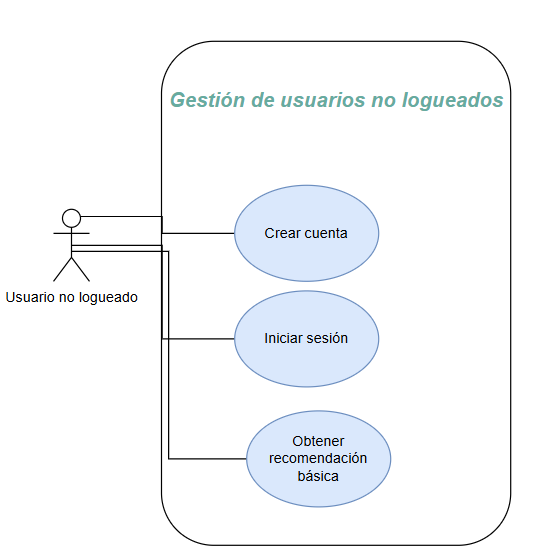
\includegraphics[width=0.75\linewidth]{imagenes/cuU.png}
    \caption{\textbf{Diagrama de casos de uso de usuario no logueado}}
    \label{casos-de-uso-ususario-no-logueado}
\end{figure}
\newpage
\subsection{Casos de uso del usuario logueado}

% Tabla: Caso de uso
\begin{table}[H]
\centering
\begin{tabular}{|c|p{10cm}|}
\hline
\rowcolor{green!40} \textbf{Caso de uso} & CU-04: Modificar información sobre videojuegos. \\ \hline
\rowcolor{blue!10} \textbf{Actores} & ACT-2 (Usuario logueado) \\ \hline
\rowcolor{blue!10} \textbf{Tipo} & Primario \\ \hline
\rowcolor{blue!10} \textbf{Precondición} & - \\ \hline
\rowcolor{blue!10} \textbf{Poscondición} & La información sobre el usuario queda actualizada. \\ \hline
\rowcolor{blue!10} \textbf{Propósito} & Permitir que el usuario modifique su información sobre videojuegos. \\ \hline
\end{tabular}
\caption{Caso de uso de modificar información sobre videojuegos}
\end{table}

% Tabla: Flujo normal de eventos
\begin{table}[H]
\centering
\begin{tabular}{|c|p{5cm}|p{5cm}|}
\hline
\rowcolor{green!40} \textbf{Paso} & \textbf{Actor} & \textbf{Sistema} \\ \hline
\rowcolor{blue!10} 1 & El usuario escribe su modificación en texto y lo envía a los agentes. &  \\ \hline
\rowcolor{blue!10} 2 &  & El sistema recibe la petición y la envía a los agentes, quienes la procesan y toman las medidas oportunas sobre la información de videojuegos del usuario. \\ \hline
\rowcolor{blue!10} 3 &  & El sistema muestra un mensaje indicando que los cambios se han realizado correctamente. \\ \hline
\end{tabular}
\caption{Flujo de eventos del caso de uso CU-04}
\end{table}

% Tabla: Curso alterno de eventos
\begin{table}[H]
\centering
\begin{tabular}{|p{4cm}|p{8cm}|}
\hline
\rowcolor{green!40} \textbf{Curso alterno de eventos} & \textbf{Descripción} \\ \hline
\rowcolor{blue!10} 2a. El texto del usuario no es correcto o está vacío. & El sistema muestra un mensaje de error indicando que el mensaje no es válido. \\ \hline
\end{tabular}
\caption{Curso alternativo del caso de uso CU-04}
\end{table}

% Tabla: Caso de uso
\begin{table}[H]
\centering
\begin{tabular}{|c|p{10cm}|}
\hline
\rowcolor{green!40} \textbf{Caso de uso} & CU-05: Modificar información sobre la cuenta. \\ \hline
\rowcolor{blue!10} \textbf{Actores} & ACT-2 (Usuario logueado) \\ \hline
\rowcolor{blue!10} \textbf{Tipo} & Secundario \\ \hline
\rowcolor{blue!10} \textbf{Precondición} & - \\ \hline
\rowcolor{blue!10} \textbf{Poscondición} & La información sobre la cuenta del usuario queda actualizada. \\ \hline
\rowcolor{blue!10} \textbf{Propósito} & Permitir al usuario modificar su contraseña o nombre de usuario. \\ \hline
\end{tabular}
\caption{Caso de uso de modificar información sobre la cuenta del usuario}
\end{table}

% Tabla: Flujo normal de eventos
\begin{table}[H]
\centering
\begin{tabular}{|c|p{5cm}|p{5cm}|}
\hline
\rowcolor{green!40} \textbf{Paso} & \textbf{Actor} & \textbf{Sistema} \\ \hline
\rowcolor{blue!10} 1 &  & El sistema pide al usuario la contraseña actual. \\ \hline
\rowcolor{blue!10} 2 & El usuario escribe la contraseña actual. & \\ \hline
\rowcolor{blue!10} 3 & El usuario escribe la nueva contraseña y/o el nuevo nombre de usuario. & \\ \hline
\rowcolor{blue!10} 4 &  & El sistema recibe los datos y efectúa el cambio. \\ \hline
\end{tabular}
\caption{Flujo de eventos del caso de uso CU-05}
\end{table}

% Tabla: Curso alterno de eventos
\begin{table}[H]
\centering
\begin{tabular}{|p{4cm}|p{8cm}|}
\hline
\rowcolor{green!40} \textbf{Curso alterno de eventos} & \textbf{Descripción} \\ \hline
\rowcolor{blue!10} 2a. La contraseña no es correcta. & El sistema muestra un mensaje de error indicando que la contraseña es incorrecta y pide que la introduzca nuevamente. \\ \hline
\rowcolor{blue!10} 4a. La nueva contraseña no cumple con los requisitos y/o el nuevo nombre de usuario ya está en uso. & El sistema muestra un mensaje de error indicando que la contraseña no cumple con los requisitos y/o el nuevo nombre de usuario ya está en uso, y pide que se modifiquen los datos. \\ \hline
\end{tabular}
\caption{Curso alternativo del caso de uso CU-05}
\end{table}

% Tabla: Caso de uso
\begin{table}[H]
\centering
\begin{tabular}{|c|p{10cm}|}
\hline
\rowcolor{green!40} \textbf{Caso de uso} & CU-06: Eliminar cuenta. \\ \hline
\rowcolor{blue!10} \textbf{Actores} & ACT-2 (Usuario logueado) \\ \hline
\rowcolor{blue!10} \textbf{Tipo} & Primario \\ \hline
\rowcolor{blue!10} \textbf{Precondición} & - \\ \hline
\rowcolor{blue!10} \textbf{Poscondición} & La cuenta y los datos del usuario han sido eliminados. \\ \hline
\rowcolor{blue!10} \textbf{Propósito} & Eliminar la cuenta del usuario. \\ \hline
\end{tabular}
\caption{Caso de uso de eliminar la cuenta del usuario}
\end{table}

% Tabla: Flujo normal de eventos
\begin{table}[H]
\centering
\begin{tabular}{|c|p{5cm}|p{5cm}|}
\hline
\rowcolor{green!40} \textbf{Paso} & \textbf{Actor} & \textbf{Sistema} \\ \hline
\rowcolor{blue!10} 1 &  & El sistema pide al usuario la contraseña actual. \\ \hline
\rowcolor{blue!10} 2 & El usuario escribe la contraseña actual. & \\ \hline
\rowcolor{blue!10} 3 &  & El sistema pregunta si el usuario está seguro de eliminar su cuenta. \\ \hline
\rowcolor{blue!10} 4 & El usuario confirma. & \\ \hline
\rowcolor{blue!10} 5 &  & El sistema cierra sesión al usuario y borra su cuenta y su información. \\ \hline
\end{tabular}
\caption{Flujo de eventos del caso de uso CU-06}
\end{table}

% Tabla: Curso alterno de eventos
\begin{table}[H]
\centering
\begin{tabular}{|p{4cm}|p{8cm}|}
\hline
\rowcolor{green!40} \textbf{Curso alterno de eventos} & \textbf{Descripción} \\ \hline
\rowcolor{blue!10} 2a. La contraseña no es correcta. & El sistema muestra un mensaje de error indicando que la contraseña es incorrecta y la pide de nuevo al usuario. \\ \hline
\rowcolor{blue!10} 3a. El usuario no está seguro de eliminar la cuenta. & El sistema regresa al usuario a la sección anterior. \\ \hline
\end{tabular}
\caption{Curso alternativo del caso de uso CU-06}
\end{table}

% Tabla: Caso de uso
\begin{table}[H]
\centering
\begin{tabular}{|c|p{10cm}|}
\hline
\rowcolor{green!40} \textbf{Caso de uso} & CU-07: Obtener datos con API externa. \\ \hline
\rowcolor{blue!10} \textbf{Actores} & ACT-2 (Usuario logueado) \\ \hline
\rowcolor{blue!10} \textbf{Tipo} & Primario \\ \hline
\rowcolor{blue!10} \textbf{Precondición} & Tener una cuenta en la plataforma externa. \\ \hline
\rowcolor{blue!10} \textbf{Poscondición} & La plataforma obtiene y guarda los datos de videojuegos de la plataforma externa. \\ \hline
\rowcolor{blue!10} \textbf{Propósito} & Obtener información de plataformas externas. \\ \hline
\end{tabular}
\caption{Caso de uso de obtener datos con API externa}
\end{table}

% Tabla: Flujo normal de eventos
\begin{table}[H]
\centering
\begin{tabular}{|c|p{5cm}|p{5cm}|}
\hline
\rowcolor{green!40} \textbf{Paso} & \textbf{Actor} & \textbf{Sistema} \\ \hline
\rowcolor{blue!10} 1 & El usuario pide conectarse a la API. &  \\ \hline
\rowcolor{blue!10} 2 &  & El sistema llama a la API. \\ \hline
\rowcolor{blue!10} 3 &  & \#Include api. \\ \hline
\rowcolor{blue!10} 4 &  & El sistema recibe el resultado de la API y almacena la información obtenida. \\ \hline
\end{tabular}
\caption{Flujo de eventos del caso de uso CU-07}
\end{table}

% Tabla: Caso de uso
\begin{table}[H]
\centering
\begin{tabular}{|c|p{10cm}|}
\hline
\rowcolor{green!40} \textbf{Caso de uso} & CU-08: Obtener recomendaciones personalizadas. \\ \hline
\rowcolor{blue!10} \textbf{Actores} & ACT-2 (Usuario logueado) \\ \hline
\rowcolor{blue!10} \textbf{Tipo} & Primario \\ \hline
\rowcolor{blue!10} \textbf{Precondición} & - \\ \hline
\rowcolor{blue!10} \textbf{Poscondición} & El usuario obtiene recomendaciones según su información y lo preguntado. \\ \hline
\rowcolor{blue!10} \textbf{Propósito} & Obtener recomendaciones personalizadas. \\ \hline
\end{tabular}
\caption{Caso de uso de obtener recomendaciones personalizadas}
\end{table}

% Tabla: Flujo normal de eventos
\begin{table}[H]
\centering
\begin{tabular}{|c|p{5cm}|p{5cm}|}
\hline
\rowcolor{green!40} \textbf{Paso} & \textbf{Actor} & \textbf{Sistema} \\ \hline
\rowcolor{blue!10} 1 & El usuario escribe su petición. &  \\ \hline
\rowcolor{blue!10} 2 &  & El sistema pasa la petición a los procesadores de lenguaje junto a la información del usuario, y estos la procesan, almacenan y crean una respuesta. \\ \hline
\rowcolor{blue!10} 3 &  & El sistema devuelve la respuesta al usuario. \\ \hline
\end{tabular}
\caption{Flujo de eventos del caso de uso CU-08}
\end{table}

% Tabla: Curso alterno de eventos
\begin{table}[H]
\centering
\begin{tabular}{|p{4cm}|p{8cm}|}
\hline
\rowcolor{green!40} \textbf{Curso alterno de eventos} & \textbf{Descripción} \\ \hline
\rowcolor{blue!10} 2a. & La petición es invalida. El sistema pide  al usuario que la introduzca de nuevo.\\ \hline
\end{tabular}
\caption{Curso alternativo del caso de uso CU-08}
\end{table}
\newpage
\subsection{Casos de usos de administrador}

Similar ausuario logueado, pero con acceso a información de debugueo, opciones especiales...

% Tabla: Caso de uso
\begin{table}[H]
\centering
\begin{tabular}{|c|p{10cm}|}
\hline
\rowcolor{green!40} \textbf{Caso de uso} & CU-09: Opciones avanzadas y obtener métricas. \\ \hline
\rowcolor{blue!10} \textbf{Actores} & ACT-3 (Administrador) \\ \hline
\rowcolor{blue!10} \textbf{Tipo} & Primario \\ \hline
\rowcolor{blue!10} \textbf{Precondición} & - \\ \hline
\rowcolor{blue!10} \textbf{Poscondición} & El administrador obtiene métricas. \\ \hline
\rowcolor{blue!10} \textbf{Propósito} & Obtener métricas y ejecutar opciones avanzadas. \\ \hline
\rowcolor{blue!10} \textbf{Extiende} & CU-04 $\rightarrow$ CU-09.\\ \hline
\end{tabular}
\caption{Caso de uso de Opciones avanzadas y obtener métricas}
\end{table}

% Tabla: Flujo normal de eventos
\begin{table}[H]
\centering
\begin{tabular}{|c|p{5cm}|p{5cm}|}
\hline
\rowcolor{green!40} \textbf{Paso} & \textbf{Actor} & \textbf{Sistema} \\ \hline
\rowcolor{blue!10} 1 & El administrador pide ejecutar un método, con posibles opciones avanzadas. &  \\ \hline
\rowcolor{blue!10} 2 &  & El sistema ejecuta ese método con las opciones avanzadas especificadas, además de ofrecer métricas. \\ \hline
\end{tabular}
\caption{Flujo de eventos del caso de uso CU-09}
\end{table}

\clearpage 

\begin{figure}[H]
    \centering
    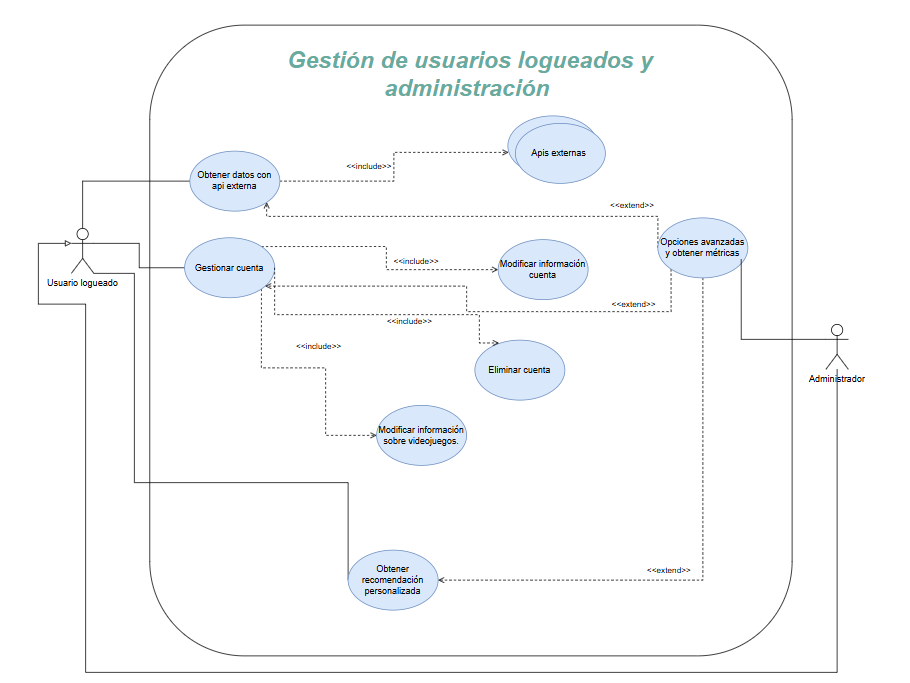
\includegraphics[width=1.3\linewidth]{imagenes/cuULYA.png}
    \caption{\textbf{Diagrama de casos de uso de usuario logueado y administrador}}
    \label{casos-de-uso-usuario-logueado}
\end{figure}









\clearpage \thispagestyle{empty} \null \clearpage
\chapter{Diseño}

En este capítulo, nos enfocaremos en el diseño de nuestra plataforma, especificando sus elementos clave, cómo se comunican entre sí y cómo optimizar su funcionamiento para sacar el máximo provecho de sus capacidades. 

También abordaremos la arquitectura general del sistema, el flujo de datos entre los distintos módulos y las decisiones de diseño tomadas para garantizar la escalabilidad, la flexibilidad y la facilidad de uso. 

En adición se considerarán aspectos relacionados con la experiencia del usuario para asegurar que la plataforma sea lo más intuitiva y eficiente.  

\newpage



\section{Diseño de la arquitectura}

A continuación, se define la arquitectura general de la plataforma, describiendo sus componentes principales y cómo se relacionan entre sí.

La arquitectura se sustenta sobre tres pilares fundamentales:

1. \textbf{Base de datos}: Es la encargada de almacenar la información del usuario, así como otros datos esenciales para el funcionamiento de la aplicación. Se comunica directamente con el backend, enviando y recibiendo información según sea necesario.

2. \textbf{Backend}: Responsable de la lógica y el procesamiento de los datos de la plataforma. En esta capa se encuentra integrado LangChain, el eje principal de este proyecto. El backend se comunica con la base de datos, enviando peticiones y  controlando el flujo de datos. En la capa superior, llamada controlador, se gestiona la comunicación con el frontend, recibiendo solicitudes y transmitiendo los datos necesarios.

3. \textbf{Frontend}: Se encarga de la presentación visual de la aplicación, siendo el medio con el que el usuario interactúa y visualiza la información. Se comunica con el backend para mostrar los datos al usuario y enviar nuevas solicitudes.

\begin{figure}[H]
    \centering
    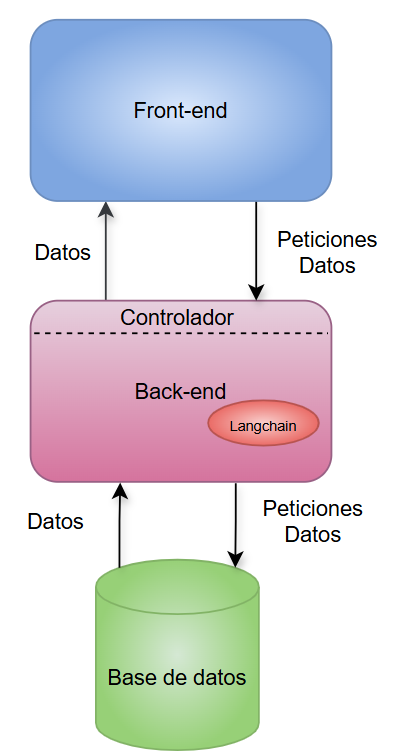
\includegraphics[width=0.5\linewidth]{imagenes/arquitectura.png}
    \caption[\textbf{Representación visual de la arquitectura}]{\textbf{Representación visual de la arquitectura}. En esta imagen se ilustran los elementos clave de la arquitectura, sus interacciones y cómo cada uno de los componentes descritos previamente se conecta y depende entre sí.}
    \label{arquitectura}
\end{figure}



\newpage

\section{Elementos de la arquitectura}

A continuación, se describen detalladamente los distintos elementos que componen la arquitectura de la plataforma.

\subsection{Base de datos}

La base de datos tiene como objetivo almacenar toda la información relevante de los usuarios. Esto incluye tanto datos personales, como nombre de usuario, contraseña o foto de perfil, como información relacionada con su actividad en videojuegos: consolas que posee, componentes de su PC, juegos jugados, títulos que le han gustado o no, suscripciones activas, así como datos proporcionados por APIs externas (por ejemplo, número de horas jugadas) o necesidades especiales que el usuario haya indicado.

Esta información debe almacenarse de forma segura, garantizando tanto la integridad ante posibles pérdidas de datos como la protección de información sensible, especialmente las contraseñas.

Asimismo, la base de datos debe ser capaz de gestionar peticiones de forma rápida y eficiente, permitiendo operaciones de lectura, inserción y modificación de datos sin comprometer el rendimiento del sistema.

En definitiva, la base de datos debe garantizar la disponibilidad, consistencia, flexibilidad y seguridad de la información en todo momento.


\subsection{Backend}

El backend es el núcleo funcional de la plataforma, encargado de procesar la lógica de la aplicación, gestionar los datos de los usuarios y coordinar la comunicación entre el frontend, la base de datos y los modelos de lenguaje.

Una de sus principales responsabilidades es la gestión de usuarios. Para ello, debe mantener un modelo interno que represente al usuario actual, proporcionando métodos que permitan modificar su información, sincronizar los cambios con la base de datos, y manejar correctamente el estado de sesión. Además, debe facilitar el envío y recepción de datos al frontend de manera eficiente y segura.

Otro aspecto central del backend es el sistema de recomendación basado en \texttt{LangChain}. Cuando el usuario realiza una solicitud (por ejemplo, pedir una recomendación de juegos), el backend debe encargarse de preparar el contexto necesario, incluyendo los datos del usuario (si está autenticado), y enviarlo a LangChain. El modelo generará una respuesta personalizada, que luego será procesada y enviada al frontend para su visualización.

En esta capa también se define la configuración de los modelos generativos de lenguajes implicados, cómo interactúan entre sí y cómo se les indica qué tarea deben realizar. Esto incluye desde la selección de cadenas de herramientas hasta el uso de agentes, dependiendo del flujo de la conversación o la consulta del usuario.

El controlador, ubicado en la parte superior del backend, actúa como intermediario entre el frontend y las capas lógicas inferiores. Expone una serie de métodos que permiten al frontend obtener y enviar datos, mientras que las capas inferiores se encargan de realizar operaciones sobre la base de datos y gestionar la lógica de recomendación.

En conjunto, el backend asegura que la plataforma funcione correctamente, manteniendo la coherencia de los datos, ejecutando las operaciones necesarias y respondiendo de forma eficaz a las interacciones del usuario.



\subsection{Frontend}

El frontend es la capa visual de la plataforma y el punto de interacción directa con el usuario. Su diseño debe priorizar la usabilidad, la claridad en la presentación de la información y la adaptación a distintos dispositivos. Para ello, es fundamental distribuir correctamente los elementos en pantalla, emplear una paleta de colores agradable y coherente, y aplicar un diseño responsivo que se adapte a diferentes resoluciones y tamaños de pantalla.

La interfaz contará con una página principal accesible para todos los usuarios, en la que podrán iniciar sesión, registrarse o acceder a una recomendación sencilla sin necesidad de autenticarse. Una vez que el usuario haya iniciado sesión, podrá acceder a funcionalidades más avanzadas, como la edición de su información personal, la solicitud de recomendaciones personalizadas o la consulta de contenido actualizado. Este contenido incluirá noticias destacadas, últimos lanzamientos adaptados a sus consolas y juegos favoritos, o recomendaciones populares entre usuarios con intereses similares.

Desde el punto de vista técnico, el frontend debe comunicarse con el backend mediante peticiones al controlador. A través de estas peticiones podrá recuperar la información necesaria (como recomendaciones o datos del perfil del usuario) y enviar nuevos datos introducidos por el usuario, como actualizaciones de su perfil o nuevas preferencias.

El diseño del frontend no solo debe ser estéticamente atractivo, sino también funcional, guiando al usuario en su experiencia y facilitando la interacción con la plataforma de forma intuitiva y eficiente.


\newpage
\section{Diseño inicial de la interfaz}

Para facilitar el desarrollo de la plataforma, es útil realizar un esbozo preliminar de la interfaz con la que interactuará el usuario. En las siguientes figuras se presentan algunos bocetos que muestran cómo se espera que el usuario visualice y navegue por la plataforma.

\begin{figure}[H]
    \centering
    \fbox{%
        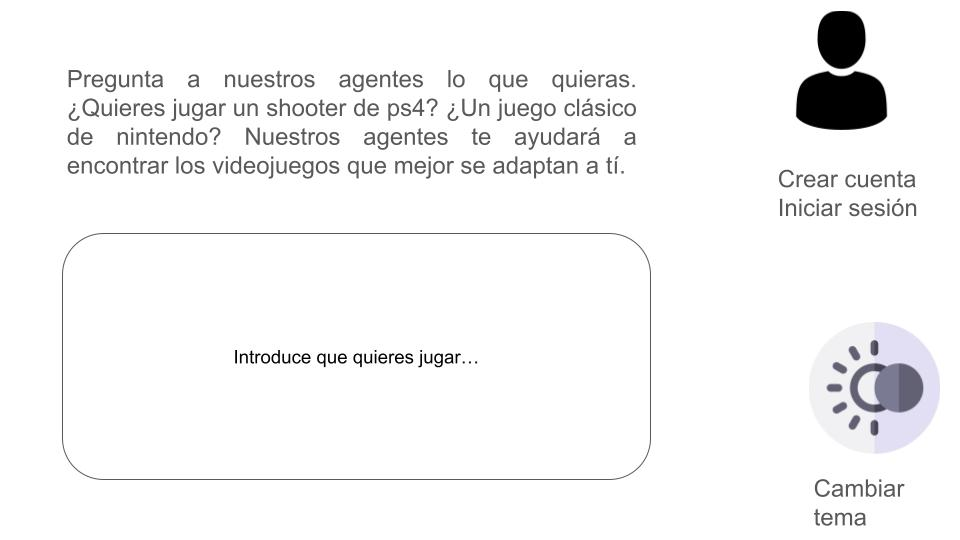
\includegraphics[width=1\linewidth]{imagenes/diPI.jpg}%
    }
    \caption{\textbf{Diseño preliminar de la página de inicio}.}
    \label{fig:pagina-inicio}
\end{figure}

\begin{figure}[H]
    \centering
    \fbox{%
        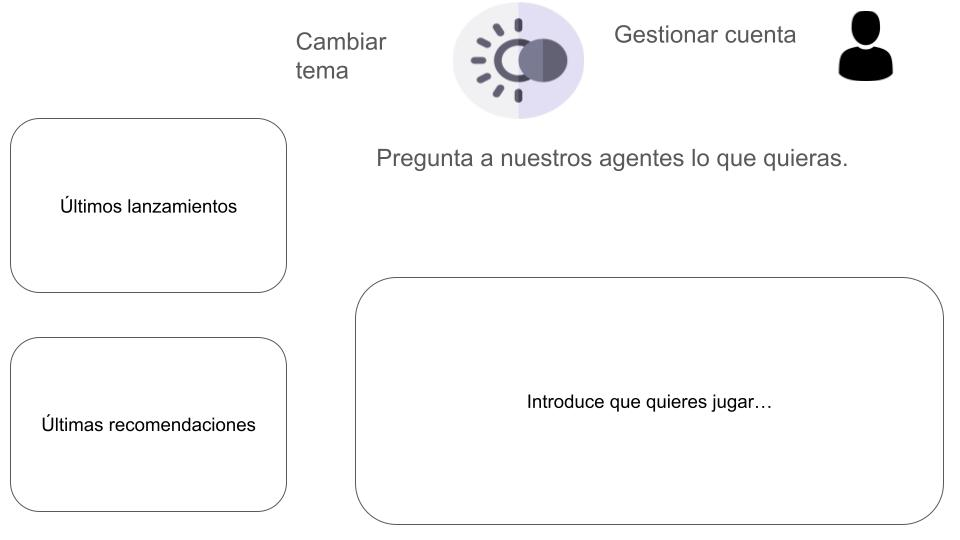
\includegraphics[width=1\linewidth]{imagenes/diPL.jpg}%
    }
    \caption{\textbf{Diseño preliminar de la página principal tras iniciar sesión}.}
    \label{fig:pagina-principal}
\end{figure}

\begin{figure}[H]
    \centering
    \fbox{%
        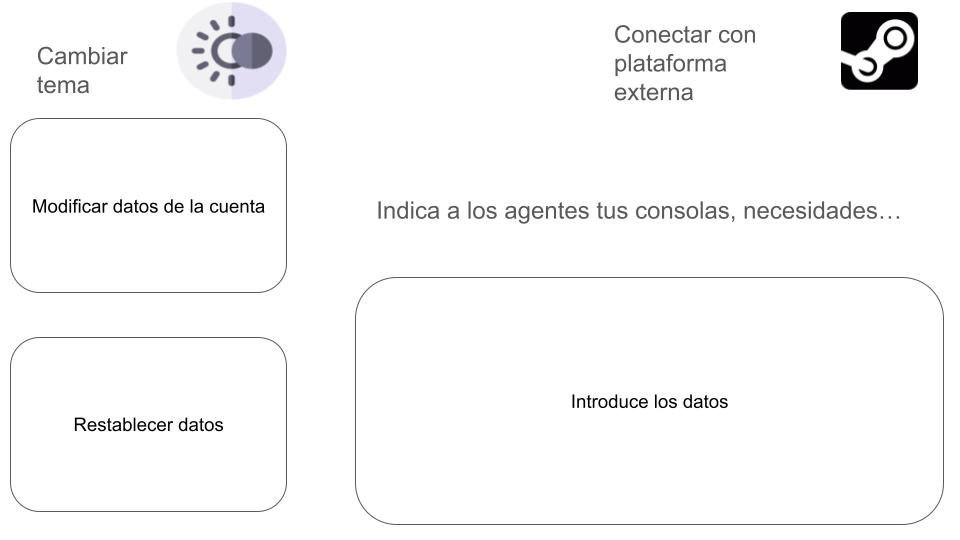
\includegraphics[width=1\linewidth]{imagenes/diA.jpg}%
    }
    \caption{\textbf{Diseño preliminar de la página de ajustes}.}
    \label{fig:pagina-ajustes}
\end{figure}


\clearpage \thispagestyle{empty} \null \clearpage
\chapter{Implementación}

En este capítulo, nos centraremos en la implementación del diseño detallado en el capítulo anterior. 

Describiremos los pasos y técnicas utilizadas para llevar a cabo la construcción de la plataforma, desde la configuración del entorno de desarrollo hasta la integración de los diferentes componentes del sistema. 

También se detallará el proceso de programación, las herramientas empleadas y las decisiones técnicas tomadas para asegurar que el diseño se traduzca eficazmente en una solución funcional. 

Además, abordaremos los retos encontrados durante la implementación y las soluciones adoptadas.




\newpage

\section{Sistema operativo}

Para el desarrollo de la plataforma se ha utilizado el sistema operativo Ubuntu, en concreto su versión 24.04.

Ubuntu es una distribución de Linux orientada al software libre y a la facilidad de uso. Es gratuita, fácil de instalar y ampliamente utilizada en el ámbito académico, especialmente en titulaciones relacionadas con la informática como la nuestra.

Además, gracias al uso de un script ejecutable, es posible instalar fácilmente todas las dependencias necesarias para el proyecto, lo que facilita la configuración del entorno de desarrollo en otros equipos.

\begin{figure}[H]
    \centering
    
\includegraphics[width=1\linewidth]{imagenes/ubuntuLogo.jpg}
    \caption[\textbf{Logo de Ubuntu}.]{\textbf{Logo de Ubuntu}. Una de las mejores distribuciones de Linux, gratuita e ideal para programadores. \href{https://www.drouiz.com/wp-content/uploads/2015/12/ubuntu-logo2.jpg}{https://www.drouiz.com/wp-content/uploads/2015/12/ubuntu-logo2.jpg}.}
    \label{logo-ubuntu}
\end{figure}

\newpage


\section{GitHub}

Para mantener nuestro trabajo seguro, con posibilidad de recuperar versiones anteriores y documentar adecuadamente los cambios realizados, utilizamos GitHub como sistema de control de versiones.

GitHub permite crear un repositorio que contiene todos los archivos del proyecto. Este repositorio puede clonarse en cualquier ordenador, facilitando así el trabajo colaborativo o desde distintos entornos. Una de sus principales funcionalidades es la posibilidad de crear distintas ramas, lo que permite, por ejemplo, desarrollar nuevas funcionalidades o corregir bugs de forma aislada. Posteriormente, estos cambios pueden fusionarse con la rama principal, conservando un historial detallado de versiones.

Gracias a GitHub, no solo almacenamos nuestro trabajo de forma remota en la nube, sino que también facilitamos el control de cambios, la colaboración con otras personas y la organización del desarrollo del proyecto.

El enlace al repositorio del proyecto es el siguiente: \url{https://github.com/juuaann03/TFG}


\begin{figure}[H]
     \centering
     
\includegraphics[width=1\linewidth]{imagenes/gitHubLogo.jpg}
     \caption[\textbf{Logo de GitHub}.]{\textbf{Logo de GitHub}. GitHub es una plataforma gratuita de desarrollo colaborativo que permite a los programadores gestionar proyectos y compartir códigos de manera eficiente y segura. \href{https://cdn.prod.website-files.com/5f5a53e153805db840dae2db/64e79ca5aff2fb7295bfddf9_github-que-es.jpg}{https://cdn.prod.website-files.com/5f5a53e153805db840dae2db/64e79ca5aff2fb7295bfddf9\_github-que-es.jpg}.}
     \label{logo-github}
 \end{figure}


\newpage


\section{Entorno de desarrollo}

Para el desarrollo de la plataforma se ha utilizado un entorno de desarrollo integrado (IDE), concretamente Visual Studio Code.

Un entorno de desarrollo proporciona un conjunto de herramientas que facilitan la programación, tales como la visualización estructurada de archivos, resaltado de sintaxis, autocompletado, depuración, y la integración directa con sistemas de control de versiones como Git y GitHub.

Visual Studio Code es un IDE moderno, ligero y altamente configurable, compatible con una amplia variedad de lenguajes de programación. Ofrece una gran cantidad de extensiones, incluyendo soporte avanzado para Python, HTML, JavaScript... Además, su integración con Git y GitHub permite realizar operaciones de control de versiones de forma sencilla y eficiente desde el propio editor.

Su interfaz intuitiva y su flexibilidad lo convierten en una herramienta ideal para el desarrollo de nuestra plataforma.

\begin{figure}[H]
     \centering
    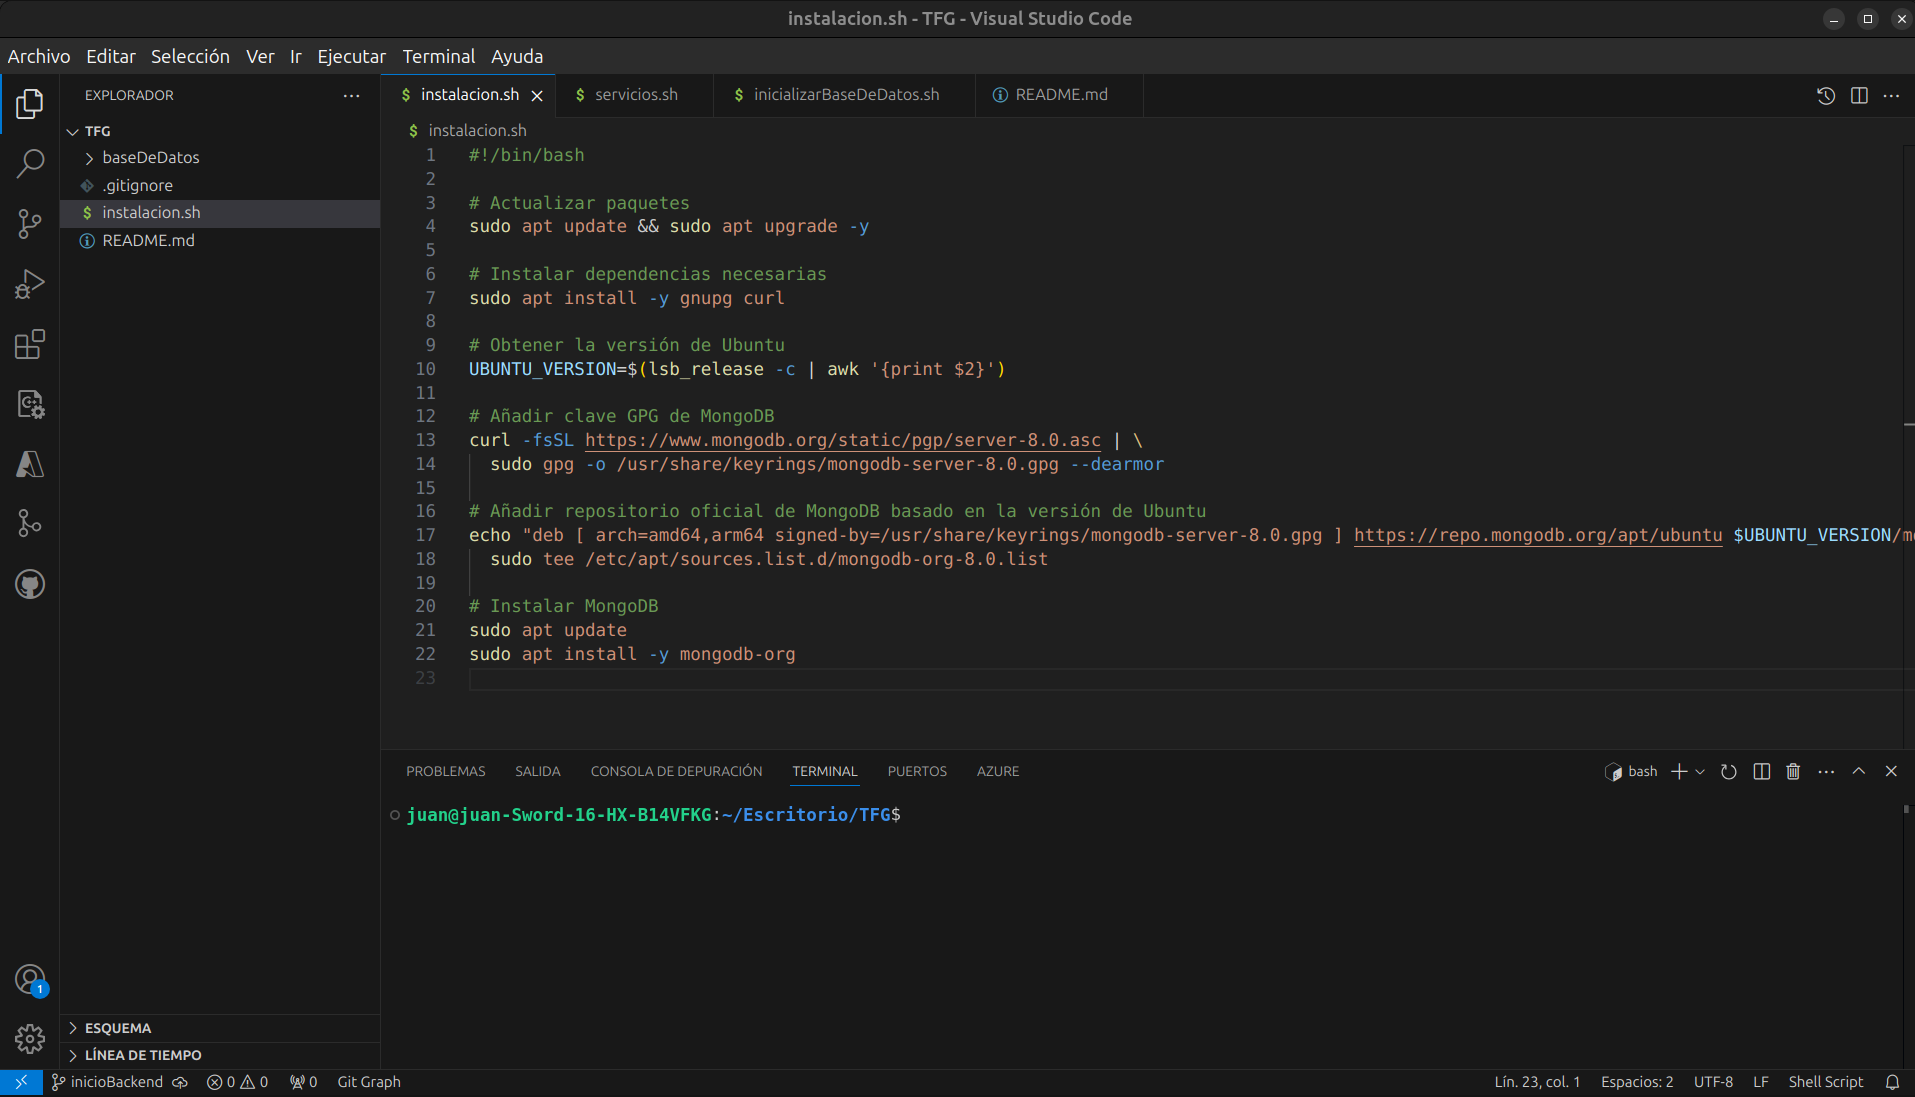
\includegraphics[width=1\linewidth]{imagenes/vc.png}
     \caption[\textbf{Interfaz de Visual Studio Code}.]{\textbf{Interfaz de Visual Studio Code}. Su interfaz es llamativa, limpia, intuitiva y personalizable. Permite ver todos los archivos de manera estructurada, gestionar las ramas de Git y resolver los conflictos de manera fácil y eficiente, entre otras funciones muy útiles.}
     \label{fig:visualStudio-label}
 \end{figure}


\newpage

\section{Base de datos: MongoDB}

Para el almacenamiento de datos en nuestra plataforma, se ha optado por utilizar \textbf{MongoDB}, una base de datos NoSQL ampliamente utilizada debido a su potencia, escalabilidad y flexibilidad. MongoDB almacena los datos en documentos BSON (una representación binaria de JSON), lo cual permite una estructura de datos más dinámica en comparación con las bases de datos relacionales tradicionales.

Una de las principales ventajas de MongoDB es su capacidad para manejar documentos con esquemas variables. Por ejemplo, un usuario puede tener 20 videojuegos marcados como favoritos, otro usuario solo 5, y otro ninguno, sin que ello suponga un problema a nivel de estructura de base de datos. Además, permite añadir o eliminar campos fácilmente durante el desarrollo sin necesidad de redefinir esquemas rígidos, algo que sería considerablemente más complejo en bases de datos SQL.

Para nuestra plataforma se ha creado una única base de datos denominada \textbf{LangGames} —una combinación de \textit{LangChain} y \textit{video games}— y una colección principal llamada \textbf{Usuarios}, donde se almacenan los perfiles y preferencias de los usuarios.

Con el fin de facilitar la configuración del entorno de desarrollo, se han creado tres scripts bash:

\begin{itemize}
	\item Un script para la instalación de MongoDB, que configura los repositorios oficiales y realiza la instalación de los paquetes necesarios.
	\item Un script para lanzar y habilitar el servicio de MongoDB al inicio del sistema.
	\item Un script que inicializa la base de datos \textit{LangGames} y crea la colección \textit{Usuarios}, asegurando que el sistema esté listo para su uso desde el primer momento.
\end{itemize}

\begin{figure}[H]
	\centering
	
\includegraphics[width=1\linewidth]{imagenes/mongoDBLogo.png}
	\caption[\textbf{Logo de MongoDB}.]{\textbf{Logo de MongoDB}. MongoDB es una base de datos orientada a documentos, altamente flexible y escalable, ideal para el desarrollo ágil de aplicaciones. \href{https://www.ovhcloud.com/sites/default/files/styles/large_screens_1x/public/2022-03/black.png}{https://www.ovhcloud.com/sites/default/files/styles/large\_screens\_1x/public/2022-03/black.png}.}
	\label{fig:mongodb-logo}
\end{figure}


\newpage

\section{BackEnd: Python, FastAPI y LangChain}

El backend de la plataforma ha sido desarrollado en \textbf{Python}, un lenguaje de programación interpretado, multiparadigma y de alto nivel. Su sintaxis sencilla y su extensa comunidad lo han posicionado como una de las principales opciones en el desarrollo de software moderno, especialmente en áreas como la inteligencia artificial, ciencia de datos y desarrollo web.

\begin{figure}[H]
	\centering
	
\includegraphics[width=0.5\linewidth]{imagenes/pythonLogo.png}
	\caption[\textbf{Logo de Python}.]{\textbf{Logo de Python}. Python es uno de los lenguajes de programación más populares y versátiles del panorama actual. \href{https://upload.wikimedia.org/wikipedia/commons/thumb/c/c3/Python-logo-notext.svg/640px-Python-logo-notext.svg.png}{https://upload.wikimedia.org/wikipedia/commons/thumb/c/c3/Python-logo-notext.svg/640px-Python-logo-notext.svg.png}.}
	\label{fig:python-logo}
\end{figure}

Para construir la Api que comunica el backend con el frontend, se ha utilizado la biblioteca \textbf{FastAPI}. Esta herramienta permite definir endpoints de manera declarativa y estructurada, facilitando la validación de datos mediante el uso de modelos definidos con \textit{Pydantic}. Además, gracias a su integración con herramientas como OpenAPI, proporciona una documentación automática e interactiva.

El servidor de desarrollo que ejecuta la aplicación FastAPI se gestiona mediante \textbf{Uvicorn}, un servidor ASGI (Asynchronous Server Gateway Interface) ligero y de alto rendimiento, especialmente diseñado para aplicaciones web modernas basadas en Python asíncrono.

\begin{figure}[H]
	\centering
	
\includegraphics[width=1\linewidth]{imagenes/fastapiLogo.png}
	\caption[\textbf{Logo de FastAPI}.]{\textbf{Logo de FastAPI}. FastAPI es una potente biblioteca de Python que permite construir APIs de forma rápida, sencilla y robusta. \href{https://miro.medium.com/v2/resize:fit:1200/1*gTztqjO7u5-GVx2cowVPsA.png}{https://miro.medium.com/v2/resize:fit:1200/1*gTztqjO7u5-GVx2cowVPsA.png}.}
	\label{fig:fastapi-logo}
\end{figure}

Para mantener un entorno limpio y controlado, se utiliza un \textbf{entorno virtual} de Python, el cual permite aislar las dependencias del proyecto del resto del sistema. Esto evita conflictos entre bibliotecas y facilita la portabilidad del entorno de desarrollo.

El backend incluye dos scripts bash:

\begin{itemize}
	\item \textbf{Script de instalación de Python y pip}: actualiza los paquetes del sistema e instala Python 3 junto con \texttt{pip} (el gestor de paquetes de Python) y \texttt{venv} (módulo para entornos virtuales).
	
	\item \textbf{Script de inicialización del entorno}: crea y activa un entorno virtual si no existe, instala todas las dependencias necesarias para el backend (incluyendo FastAPI, Uvicorn, LangChain y otras bibliotecas auxiliares), genera un archivo \texttt{requirements.txt} con la lista de dependencias, y lanza el servidor FastAPI en segundo plano, redirigiendo su salida a un archivo de log.
\end{itemize}

Dentro del backend se encuentra el archivo principal \texttt{main.py}, la carpeta \texttt{app/} que contiene los distintos módulos del sistema, y un archivo de entorno(.env) adicional para gestionar claves necesarias para el correcto funcionamiento de ciertas funcionalidades, cuya obtención y uso está debidamente documentada en el \texttt{README} del repositorio de GitHub.

A continuación, se describe con mayor detalle la estructura y funcionalidad de la carpeta \texttt{app/}.


\subsection{DB}

La carpeta \texttt{db} contiene un único archivo llamado \texttt{mongodb.py}, el cual se encarga de gestionar la conexión con la base de datos MongoDB.

En él se utiliza la biblioteca \texttt{pymongo} para establecer la conexión con el servidor local de MongoDB (\texttt{localhost:27017}). Una vez conectados, se selecciona la base de datos \texttt{LangGames} y se almacena la colección \texttt{Usuarios} en una variable que se puede importar fácilmente desde otros módulos del backend.

Esta estrategia favorece la reutilización y centralización del acceso a la base de datos, evitando duplicación de código y facilitando su mantenimiento.


\subsection{Utils}

Esta carpeta contiene dos archivos con funciones auxiliares esenciales para el funcionamiento del backend.

\begin{itemize}
	\item \textbf{jwt.py}: Este archivo se encarga de generar \textbf{tokens JWT (JSON Web Tokens)}, que permiten autenticar de forma segura a los usuarios. Cada vez que un usuario inicia sesión correctamente, se le genera un token que contiene su correo electrónico (u otro dato identificativo) y una fecha de expiración. Este token se firma digitalmente usando una clave secreta, de modo que el servidor pueda verificar su validez en futuras peticiones sin necesidad de mantener sesiones abiertas. Así se garantiza una comunicación segura y sin estado entre el cliente y el servidor.
	
	\item \textbf{utilidadesVarias.py}: Aquí se agrupan funciones y configuraciones de utilidad. Por ejemplo:
	\begin{itemize}
		\item Se cargan las claves necesarias para acceder a las APIs externas desde un archivo \texttt{.env}.
		\item Se definen listas con los modelos de lenguaje disponibles para su uso.
		\item \texttt{limpiar\_respuesta()}: una función que extrae y limpia la parte JSON de las respuestas generadas por modelos de lenguaje.
		\item \texttt{obtener\_imagen\_juego()}: consulta la API de RAWG para obtener automáticamente una imagen representativa del videojuego que se le indique.
	\end{itemize}
\end{itemize}


\subsection{Modelos}

Los modelos representan la estructura de los datos con los que trabaja el sistema, facilitando la organización y el intercambio de información entre distintas partes del backend.

El modelo principal es el del \textbf{usuario}, que incluye tanto los datos básicos como el nombre, correo y contraseña, como otros campos más específicos relacionados con el mundo de los videojuegos. Por ejemplo, se almacena información sobre las consolas que posee, la configuración de su ordenador, sus gustos personales, los juegos que ha jugado o que no le han gustado, e incluso su historial de los videojuegos recomendados por los modelos de lenguaje. Esta estructura permite personalizar al máximo la experiencia del usuario.

Además del modelo de usuario, se han definido otras clases auxiliares para manejar información concreta:
\begin{itemize}
	\item Modelos para solicitudes de recomendación, tanto básica como personalizada.
	\item Un modelo para representar los próximos lanzamientos de videojuegos, incluyendo su título, fecha, plataformas y una imagen asociada.
\end{itemize}

Estas clases permiten que los distintos módulos del backend se comuniquen utilizando estructuras coherentes y bien definidas, lo que facilita la validación de datos y mejora la organización del código.



\subsection{Gestores}

Los gestores se encargan de realizar las operaciones relacionadas con los datos que maneja el sistema. En este caso, contamos con un gestor centrado en los usuarios.

El \textbf{gestor de usuarios} proporciona una serie de funciones que permiten crear un nuevo usuario, obtener sus datos, modificarlos o eliminarlos. También incluye la verificación de contraseñas para el proceso de inicio de sesión y una función para limpiar los campos opcionales del perfil del usuario. Además aplica un hash a las contraseñas para que el sistema sea más seguro.

Este archivo actúa como intermediario entre la base de datos y otras partes de la aplicación, como las rutas o los servicios. Gracias a él, se centraliza la lógica relacionada con los usuarios, facilitando el mantenimiento y la reutilización del código.


\subsection{Servicios}

Los servicios se encargan de implementar las funcionalidades centrales del sistema.

El servicio de usuario actúa como intermediario entre el gestor de usuarios y los demás servicios. Su función principal es preprocesar los datos recibidos del usuario, invocar los servicios correspondientes con dichos datos y aplicar las modificaciones necesarias en el perfil.

El servicio de recomendación básica está diseñado para usuarios no autenticados que solicitan recomendaciones de videojuegos. Ante una petición, se consultan hasta tres modelos de lenguaje para obtener posibles respuestas. Si algún modelo falla, el sistema puede seguir con normalidad. Una vez obtenidas las respuestas, un modelo la sintetiza en una sola. Si el modelo falla, se sigue con los siguientes hasta que se obtiene una respuesta válida. Esta gestión secuencial de modelos se facilita mediante la biblioteca \texttt{LangChain}, que simplifica la invocación, manejo y conmutación entre modelos. Para acceder a los modelos, se utiliza \texttt{OpenRouter}, una API que permite interactuar con múltiples proveedores y modelos sin necesidad de gestionar varias claves de acceso. \texttt{OpenRouter} también ofrece una prueba gratuita limitada en tokens.

El servicio de recomendación personalizada extiende la funcionalidad básica incorporando datos específicos del usuario, como su historial de videojuegos y recomendaciones previas, para evitar redundancias. Además, este servicio puede actualizar el perfil del usuario automáticamente si la petición incluye información que modifica su estado, como la venta de una consola o la adquisición de un nuevo juego.

Por otro lado, existe un servicio dedicado exclusivamente a actualizar la información relativa a los videojuegos del usuario a partir del texto que éste proporciona. Este servicio utiliza modelos de lenguaje para analizar la petición y detectar los cambios necesarios, devolviendo una actualización precisa y estructurada.

Asimismo, contamos con dos servicios innovadores que mejoran significativamente la experiencia de usuario:

\begin{enumerate}
	\item \textbf{Servicio de próximos lanzamientos:} Este servicio obtiene información sobre videojuegos próximos a salir mediante la API de RAWG, incluyendo nombres, géneros, plataformas y imágenes. Los modelos analizan estos datos para filtrar y recomendar aquellos títulos que mejor se ajustan a los gustos del usuario.
	\item \textbf{Servicio de integración con Steam:} Mediante la API de Steam, este servicio recupera la lista de juegos poseídos por el usuario y el tiempo de juego asociado a cada uno, usando su ID de Steam. Basándonos en esta información, actualizamos el perfil del usuario, considerando que un juego está realmente jugado si el usuario ha dedicado más de una hora a jugarlo.
\end{enumerate}

\subsection{Rutas}

Las rutas permiten exponer las funcionalidades del sistema a través de peticiones HTTP, especificando el tipo de operación (\texttt{GET}, \texttt{POST}, \texttt{PUT}, \texttt{DELETE}), la ruta asociada (path), los posibles errores, y los datos requeridos o devueltos. Estas rutas actúan como puntos de entrada a los servicios internos de la aplicación, es decir, el controlador.

En el sistema se han definido rutas para distintas funcionalidades clave:

\begin{itemize}
	\item \textbf{Autenticación:} Permite a los usuarios iniciar sesión mediante la verificación de credenciales. Al autenticarse correctamente, se genera y devuelve un token JWT que puede ser utilizado en peticiones protegidas.
	
	\item \textbf{Gestión de usuarios:} Incluye rutas para crear, obtener, actualizar y eliminar usuarios, así como para modificar sus datos obligatorios u opcionales, acceder a sus preferencias y sincronizar sus datos con Steam.
	
	\item \textbf{Recomendaciones:} Ofrece rutas tanto para recomendaciones básicas (sin necesidad de estar autenticado) como para recomendaciones personalizadas basadas en el perfil y el historial del usuario.
	
	\item \textbf{Próximos lanzamientos:} Permite obtener una lista de videojuegos próximos a lanzarse, filtrados en función de los gustos del usuario, utilizando datos de la API de RAWG.
\end{itemize}

Cada ruta está asociada a un módulo independiente dentro de la aplicación, lo que favorece una organización modular y facilita el mantenimiento y la ampliación del sistema.

\subsection{Main}

El archivo \texttt{main.py} actúa como punto de entrada de la aplicación. Su función principal es inicializar el servidor web y registrar todas las rutas disponibles en el sistema. Para ello, importa los distintos módulos de rutas definidos en la aplicación y los incluye en la instancia principal de \texttt{FastAPI} mediante el método \texttt{include\_router()}.

Además, se configura el middleware de CORS (\textit{Cross-Origin Resource Sharing}) para permitir que la aplicación frontend (por ejemplo, una interfaz en Angular corriendo en \texttt{http://localhost:4200}) pueda comunicarse con el backend sin restricciones de origen.

Este archivo es esencial para arrancar el sistema y exponer todos los servicios a través de una única instancia centralizada.


\newpage

\section{FrontEnd: Angular}

El frontend de la aplicación ha sido desarrollado utilizando \textbf{Angular}, un framework de desarrollo web moderno, mantenido por Google, que facilita la creación de aplicaciones de una sola página (SPA) con una arquitectura robusta y escalable.

Angular se basa principalmente en los lenguajes \textbf{HTML}, \textbf{SCSS/CSS} y \textbf{TypeScript}. Para el diseño visual y la personalización del estilo, se ha utilizado el framework de utilidades CSS \textbf{Tailwind CSS}, que permite construir interfaces de usuario de forma rápida y flexible mediante clases predefinidas.

Al igual que las otras partes cuenta con scripts, para instalar lo necesario e inicializar el frontend en segundo plano. También cuenta con un script que se utilizó para comenzar el desarrollo.

Estos scripts simplifican considerablemente el proceso de despliegue local, garantizando que cualquier desarrollador pueda ejecutar el frontend con facilidad.

\begin{figure}[H]
	\centering
	
\includegraphics[width=1\linewidth]{imagenes/logoAngular.png}
	\caption[\textbf{Logo de Angular}.]{\textbf{Logo de Angular}. Angular es un framework completo y muy utilizado para el desarrollo de interfaces web modernas. Fuente: \href{https://media.licdn.com/dms/image/v2/D4D12AQHF0nuL7dxEOA/article-cover_image-shrink_720_1280/article-cover_image-shrink_720_1280/0/1710076882649?e=2147483647&v=beta&t=z_GWbz1UXR5oIm-mSUhdCJnspOV0vronhDj9-o7xOhI}{https://media.licdn.com/dms/image/v2/D4D12AQHF0nuL7dxEOA/article-cover\_image-shrink\_720\_1280/article-cover\_image-shrink\_720\_1280/0/1710076882649?e=2147483647\&v=beta\&t=z\_GWbz1UXR5oIm-mSUhdCJnspOV0vronhDj9-o7xOhI}.}
	\label{fig:logo-angular}
\end{figure}


Angular genera automáticamente gran parte de la estructura inicial del proyecto, lo cual permite centrarse desde el inicio en el desarrollo funcional y visual de la aplicación.

Uno de los elementos clave en la personalización del diseño es la configuración del sistema de estilos. Para ello se ha utilizado \textbf{Tailwind CSS}, que ofrece una forma muy eficiente y flexible de aplicar estilos directamente en los componentes. En este caso, se ha habilitado el modo claro y oscuro, de forma que el diseño se adapta según las preferencias del usuario. Además, se han realizado pequeños ajustes para asegurar que, incluso en campos de formularios autocompletados, los colores se mantengan coherentes con el tema activo.

La estructura principal del frontend se encuentra en la carpeta src donde reside el código fuente. Allí se definen aspectos globales como el título de la página, el icono del navegador, la dirección base de la API y los estilos que afectan a toda la aplicación.

Dentro de esta estructura se encuentra la carpeta principal del proyecto, app, que es donde se desarrolla casi toda la funcionalidad. Esta parte incluye, por ejemplo, la definición de las rutas de navegación, que permiten moverse entre las distintas vistas como el inicio, el registro o la pantalla principal tras iniciar sesión.

También se incluye un sistema de servicios en la carpeta services, que se encargan de gestionar las conexiones con la API. Uno de estos servicios, por ejemplo, permite obtener los próximos lanzamientos de videojuegos relacionados con el usuario. Estos datos se almacenan temporalmente en memoria caché para evitar repetir llamadas innecesarias, lo que mejora la eficiencia y la velocidad de la aplicación.

Además, se han definido varias \textbf{interfaces} que actúan como plantillas para los datos que se van a utilizar, como pueden ser las recomendaciones personalizadas, los lanzamientos futuros o los datos de los usuarios. Estas interfaces permiten trabajar con los datos de forma más organizada y segura.

A continuación, se describe la carpeta de \textit{componentes}, que contiene las diferentes piezas visuales y funcionales que forman la interfaz del sistema.

\subsection{Componentes}

En Angular, un componente es una de las piezas clave para construir interfaces. Cada uno representa una parte específica de la aplicación y cuenta con su propia estructura (HTML), comportamiento (TypeScript) y estilo (CSS o SCSS). Gracias a la modularidad que ofrece este enfoque, podemos construir interfaces complejas a partir de componentes más simples y reutilizables.

En nuestro caso, todos los componentes han sido diseñados pensando en la experiencia del usuario. Incluyen un botón para alternar entre modo claro y oscuro, se adaptan automáticamente a pantallas pequeñas (diseño responsive), e incorporan pequeñas animaciones que hacen la experiencia más agradable. Por ejemplo, se utiliza una Poké Ball giratoria durante las cargas normales, y un R2D2 para mostrar mientras carga los próximos lanzamientos.

A continuación, describimos cada componente de forma individual.

\subsubsection{Home}

El componente \texttt{Home} es la página principal de la aplicación. Nada más entrar, el usuario se encuentra con una cabecera que incluye el nombre de la app, su logotipo, y dos botones: uno para iniciar sesión y otro para registrarse.

En el centro de la página hay un cuadro de texto donde el usuario puede escribir qué tipo de juego está buscando. Una vez enviada la petición, se muestran las recomendaciones en formato de tarjetas. Cada tarjeta incluye una imagen del juego, su nombre, las plataformas disponibles y una breve explicación de por qué se ha recomendado ese juego en concreto.

En la parte inferior, se encuentra una sección con un segundo logotipo y el aviso de derechos de autor.

\vspace{0.5cm}

\begin{figure}[H]
	\centering
	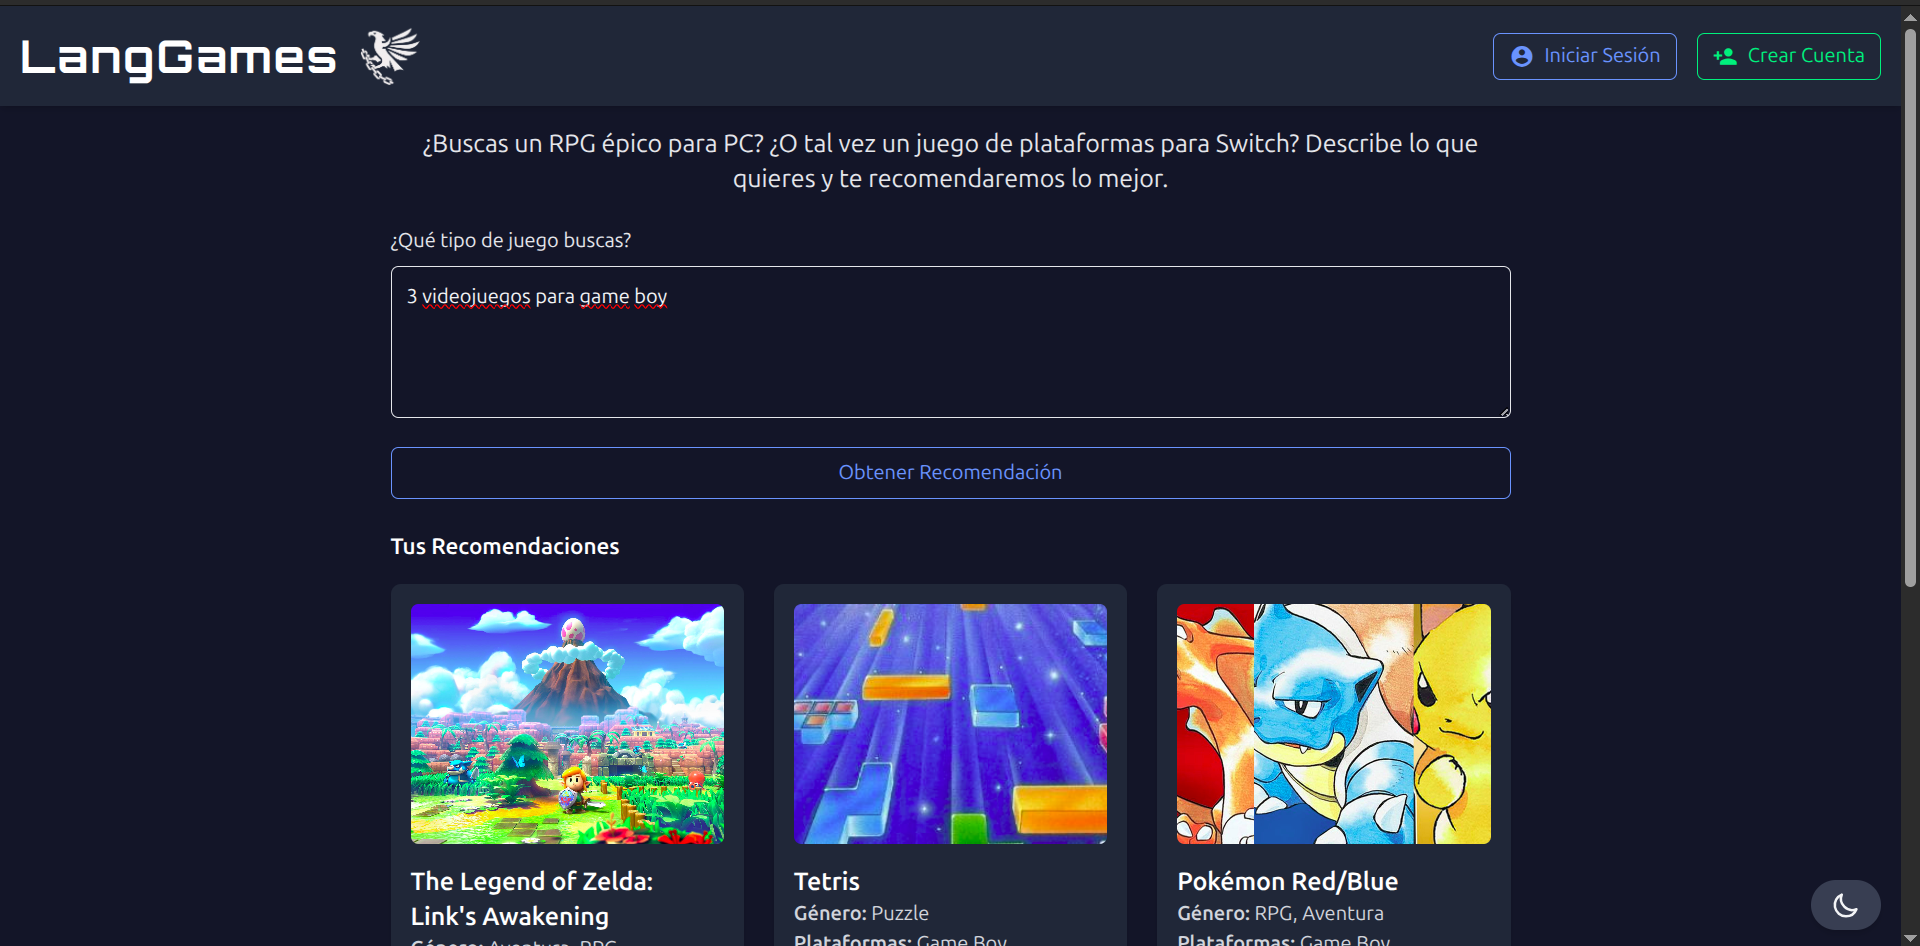
\includegraphics[width=1\linewidth]{imagenes/home1.png}
	\caption[\textbf{Imagen de home 1}.]{\textbf{Imagen de home 1}. Vista principal de la página con recomendaciones ya generadas.}
	\label{imagen-home-1}
\end{figure}

\begin{figure}[H]
	\centering
	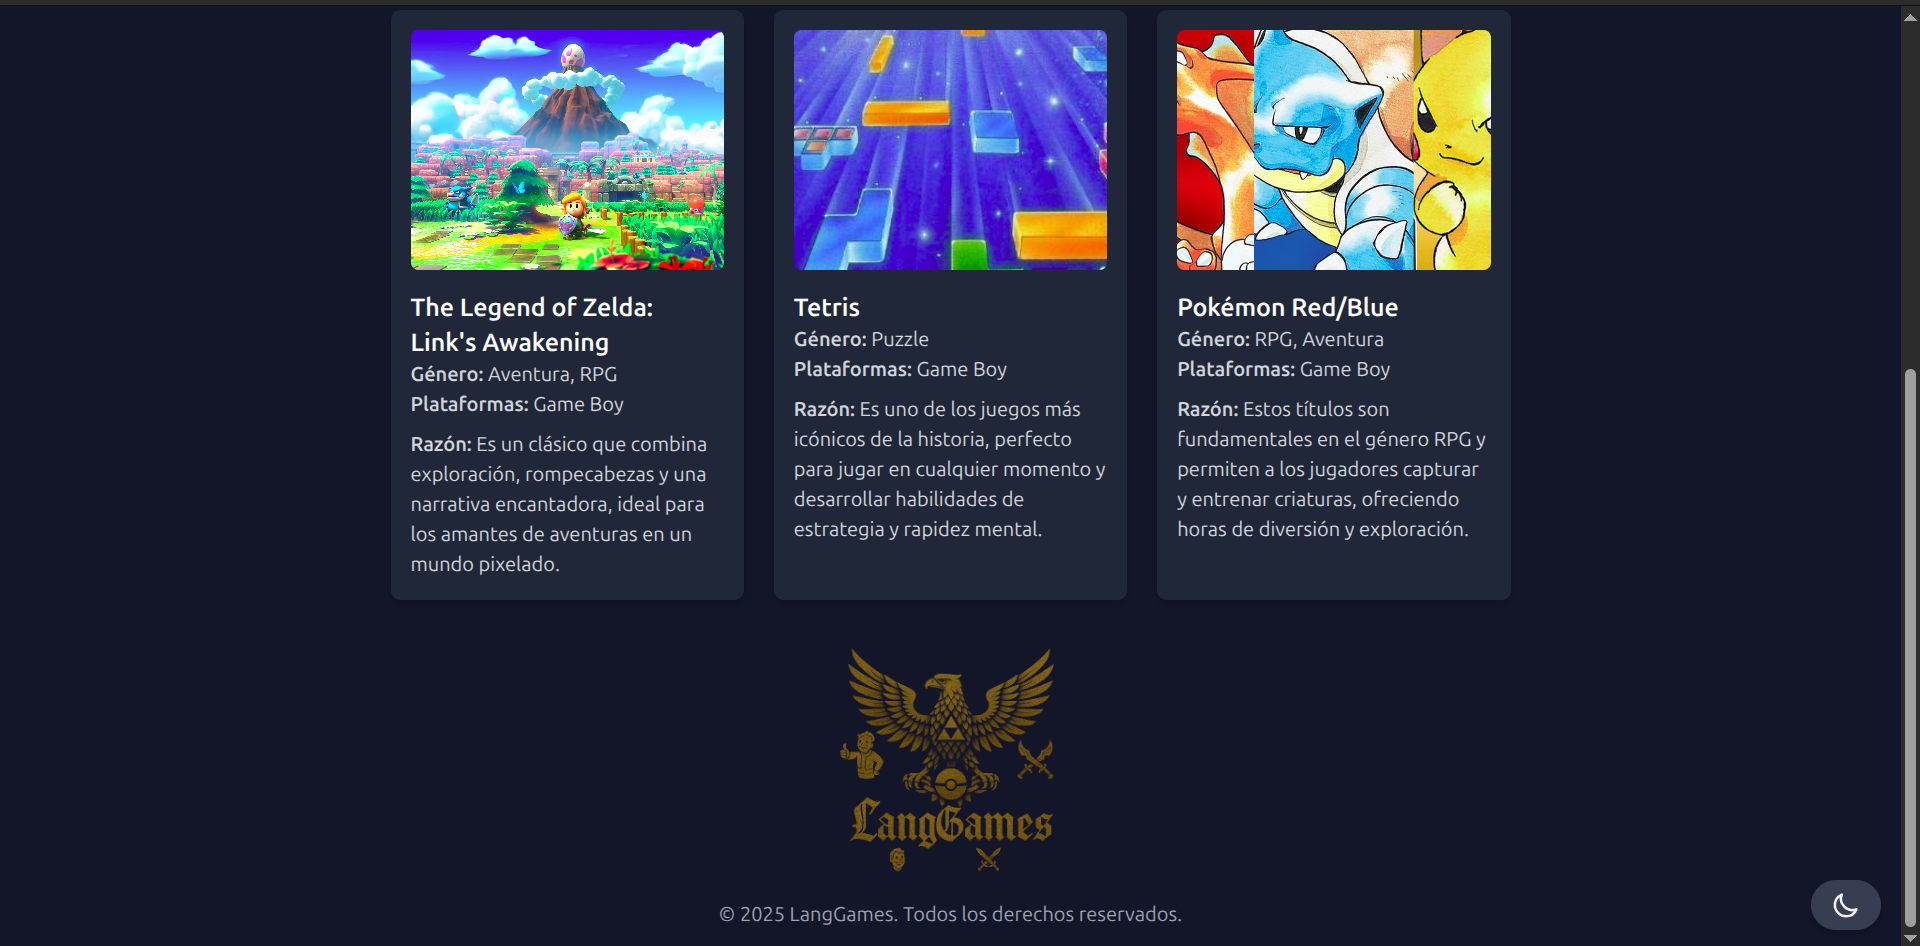
\includegraphics[width=1\linewidth]{imagenes/home2.png}
	\caption[\textbf{Imagen de home 2}.]{\textbf{Imagen de home 2}. Parte inferior de la página, con el segundo logotipo y el pie de página.}
	\label{imagen-home-2}
\end{figure}

\begin{figure}[H]
	\centering
	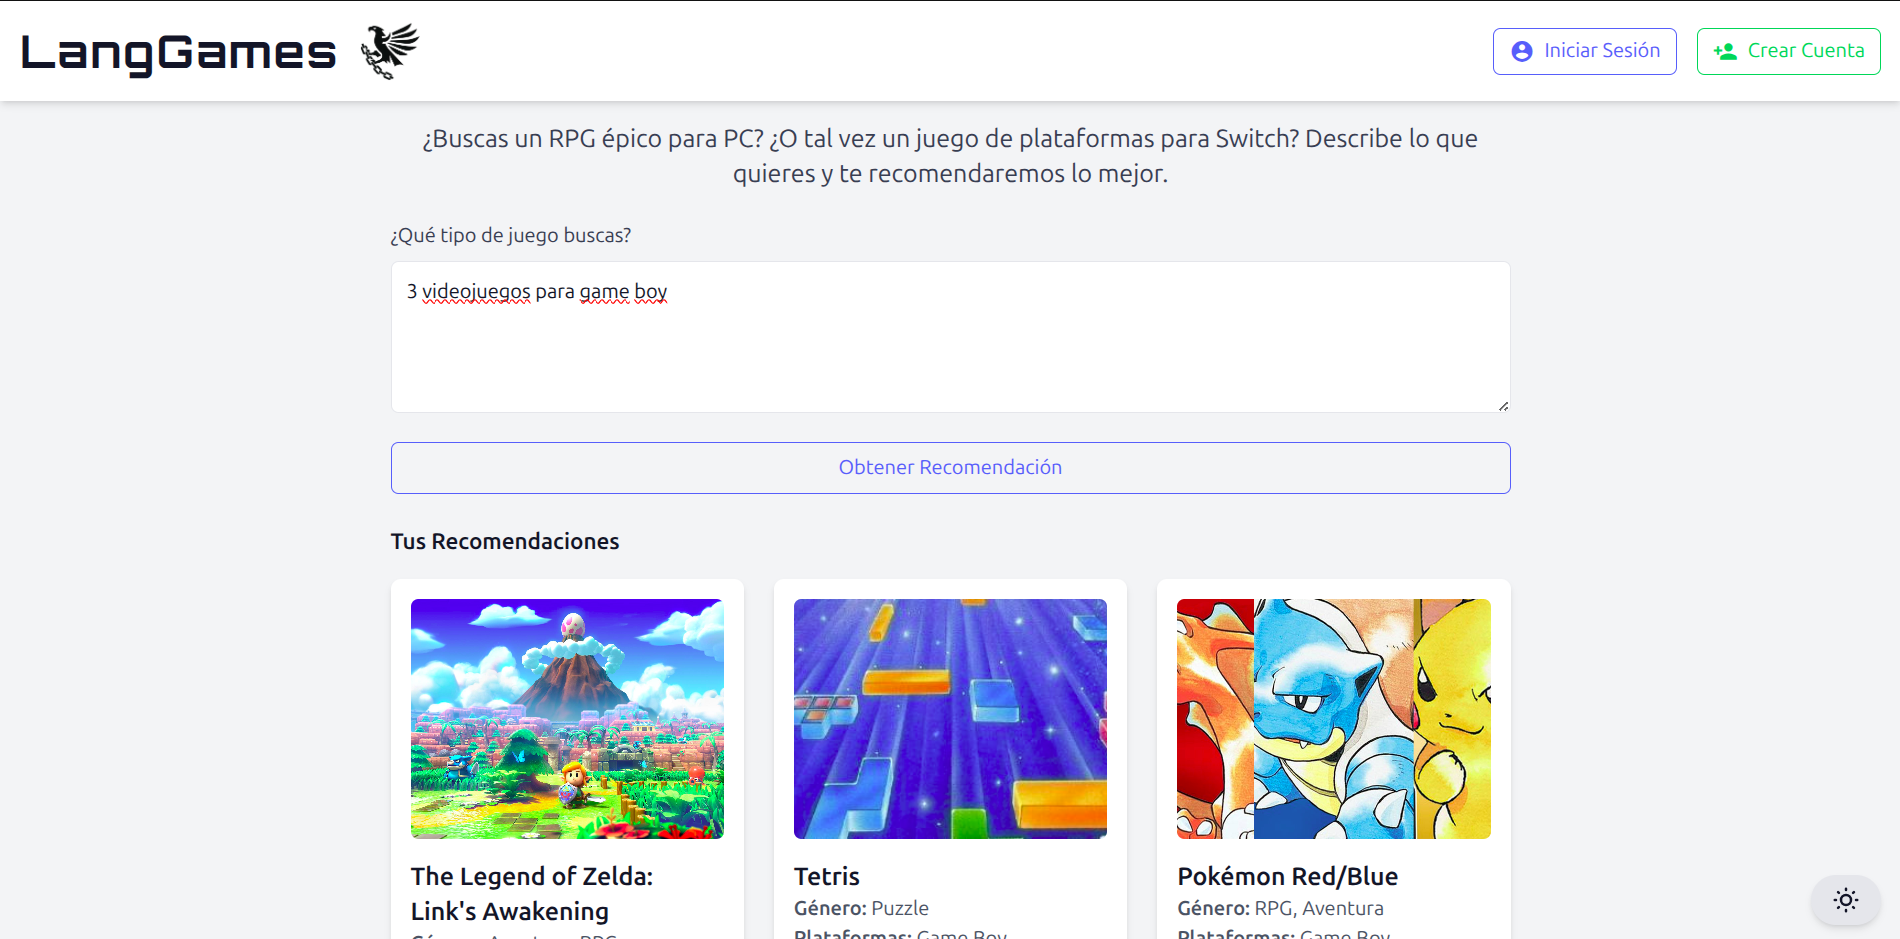
\includegraphics[width=1\linewidth]{imagenes/homeClaro.png}
	\caption[\textbf{Modo claro}.]{\textbf{Modo claro}. La aplicación ofrece tanto modo claro como oscuro, para mayor comodidad del usuario.}
	\label{imagen-home-claro}
\end{figure}

\begin{figure}[H]
	\centering
	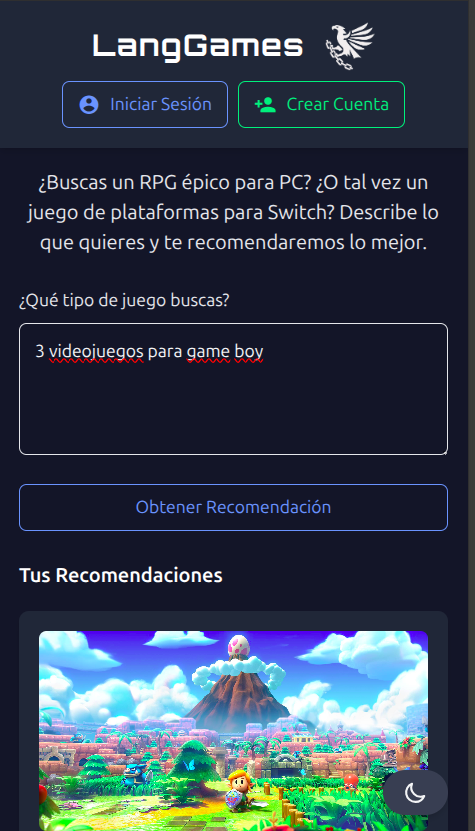
\includegraphics[width=1\linewidth]{imagenes/homeMovil1.png}
	\caption[\textbf{Vista móvil 1}.]{\textbf{Vista móvil 1}. Diseño adaptado para dispositivos móviles, con todos los elementos reorganizados.}
	\label{imagen-movil-1}
\end{figure}

\begin{figure}[H]
	\centering
	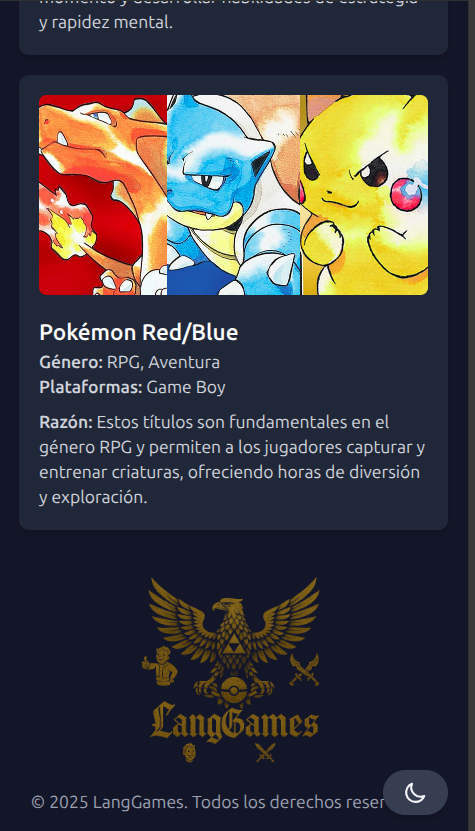
\includegraphics[width=1\linewidth]{imagenes/homeMovil2.png}
	\caption[\textbf{Vista móvil 2}.]{\textbf{Vista móvil 2}. Otra vista desde un dispositivo móvil, mostrando el aspecto del pie de página.}
	\label{imagen-movil-2}
\end{figure}



\subsubsection{Registro}

El sistema de registro permite a los usuarios crear una cuenta nueva desde una ventana superpuesta a la pantalla principal \textit{Home}. Para completar el registro, el usuario debe proporcionar un nombre de usuario, una dirección de correo electrónico válida y una contraseña segura.

El formulario valida en tiempo real que tanto el nombre como el correo electrónico no estén ya registrados en el sistema. En caso contrario, se muestra un mensaje de error al usuario indicando el conflicto.

En cuanto a la contraseña, esta debe cumplir con los siguientes requisitos mínimos:
\begin{itemize}
	\item Tener una longitud mínima de 8 caracteres.
	\item Incluir al menos una letra y un número.
\end{itemize}

Una vez completado el formulario de manera correcta y superadas todas las validaciones, el sistema crea la cuenta de usuario y realiza el inicio de sesión de forma automática, redirigiendo al usuario a la pantalla principal.

\begin{figure}[H]
	\centering
	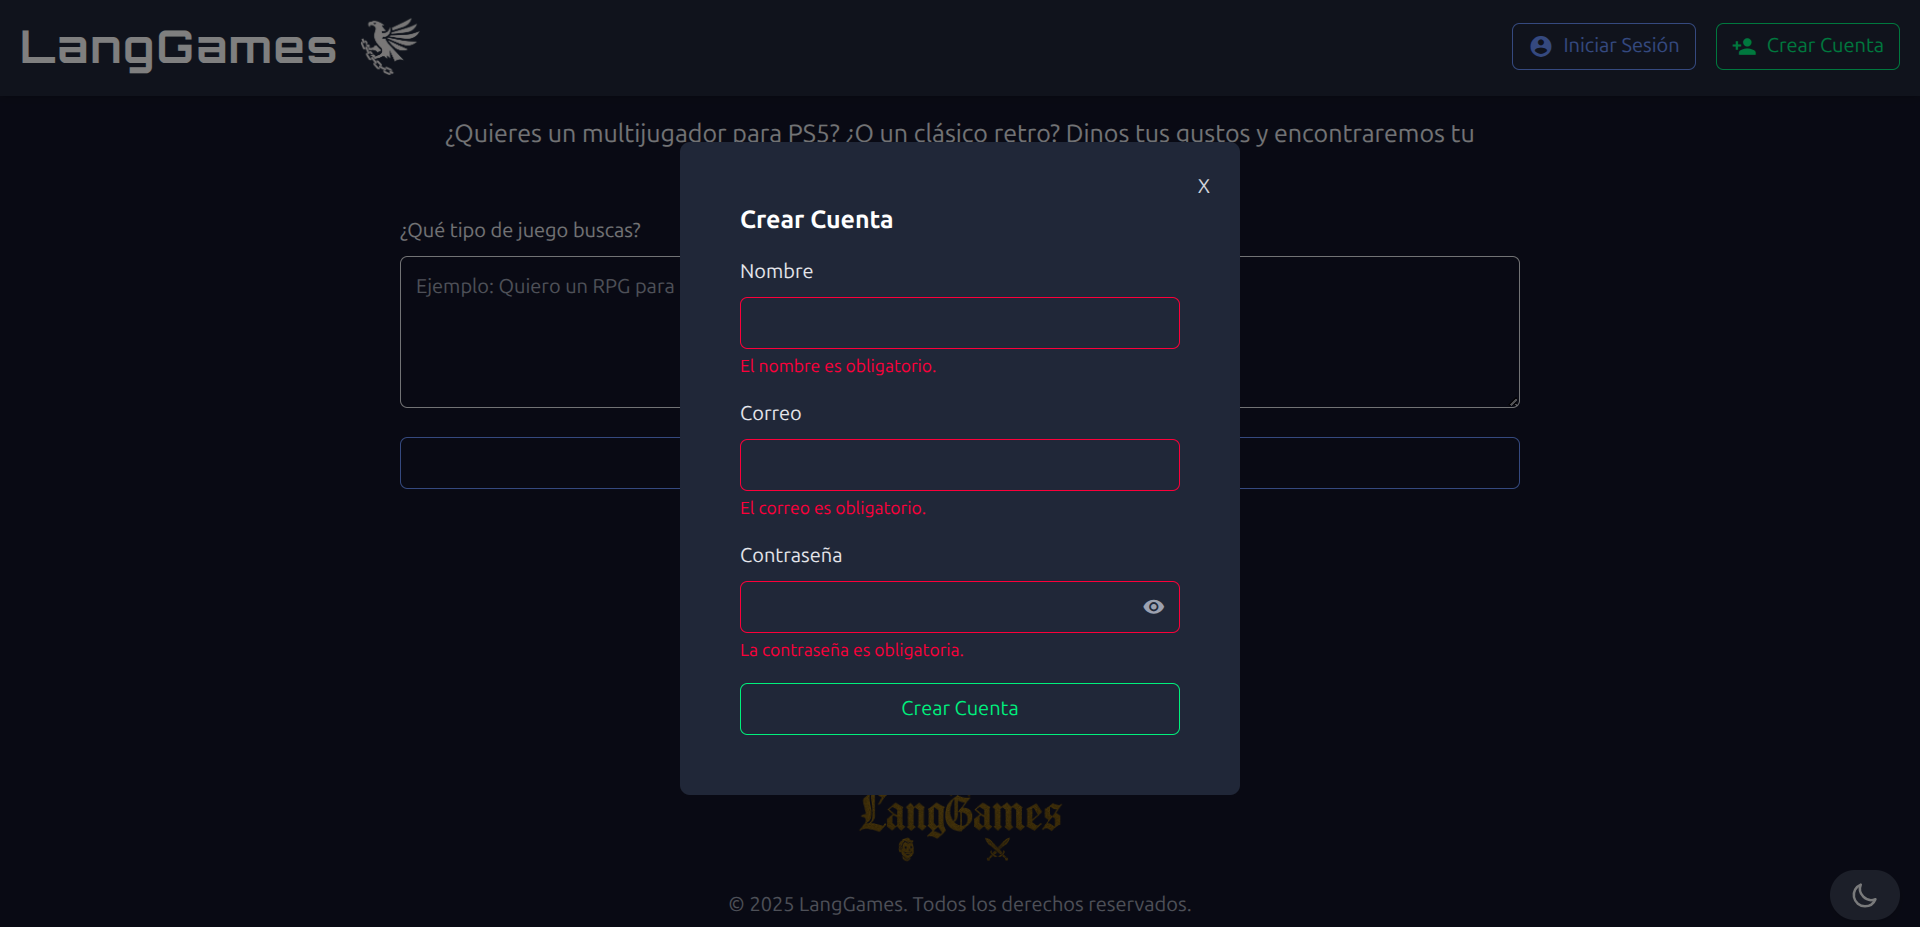
\includegraphics[width=1\linewidth]{imagenes/register.png}
	\caption[\textbf{Registro}.]{\textbf{Registro}. Formulario de creación de cuenta en la plataforma.}
	\label{imagen-register}
\end{figure}



\subsubsection{Login}

El componente de \textit{login} permite a los usuarios autenticarse en la plataforma introduciendo sus credenciales: correo electrónico y contraseña. El formulario verifica que los campos no estén vacíos y que el correo tenga un formato válido antes de enviar los datos.

En caso de que el usuario introduzca credenciales incorrectas o no esté registrado, se muestra un mensaje de error informativo. Si la autenticación es exitosa, se almacena el token de sesión, el rol del usuario, su nombre y su correo en el almacenamiento local del navegador, y se redirige automáticamente a la pantalla principal.

Además, el campo de contraseña ofrece la opción de mostrar u ocultar el texto introducido para mejorar la experiencia del usuario.

\begin{figure}[H]
	\centering
	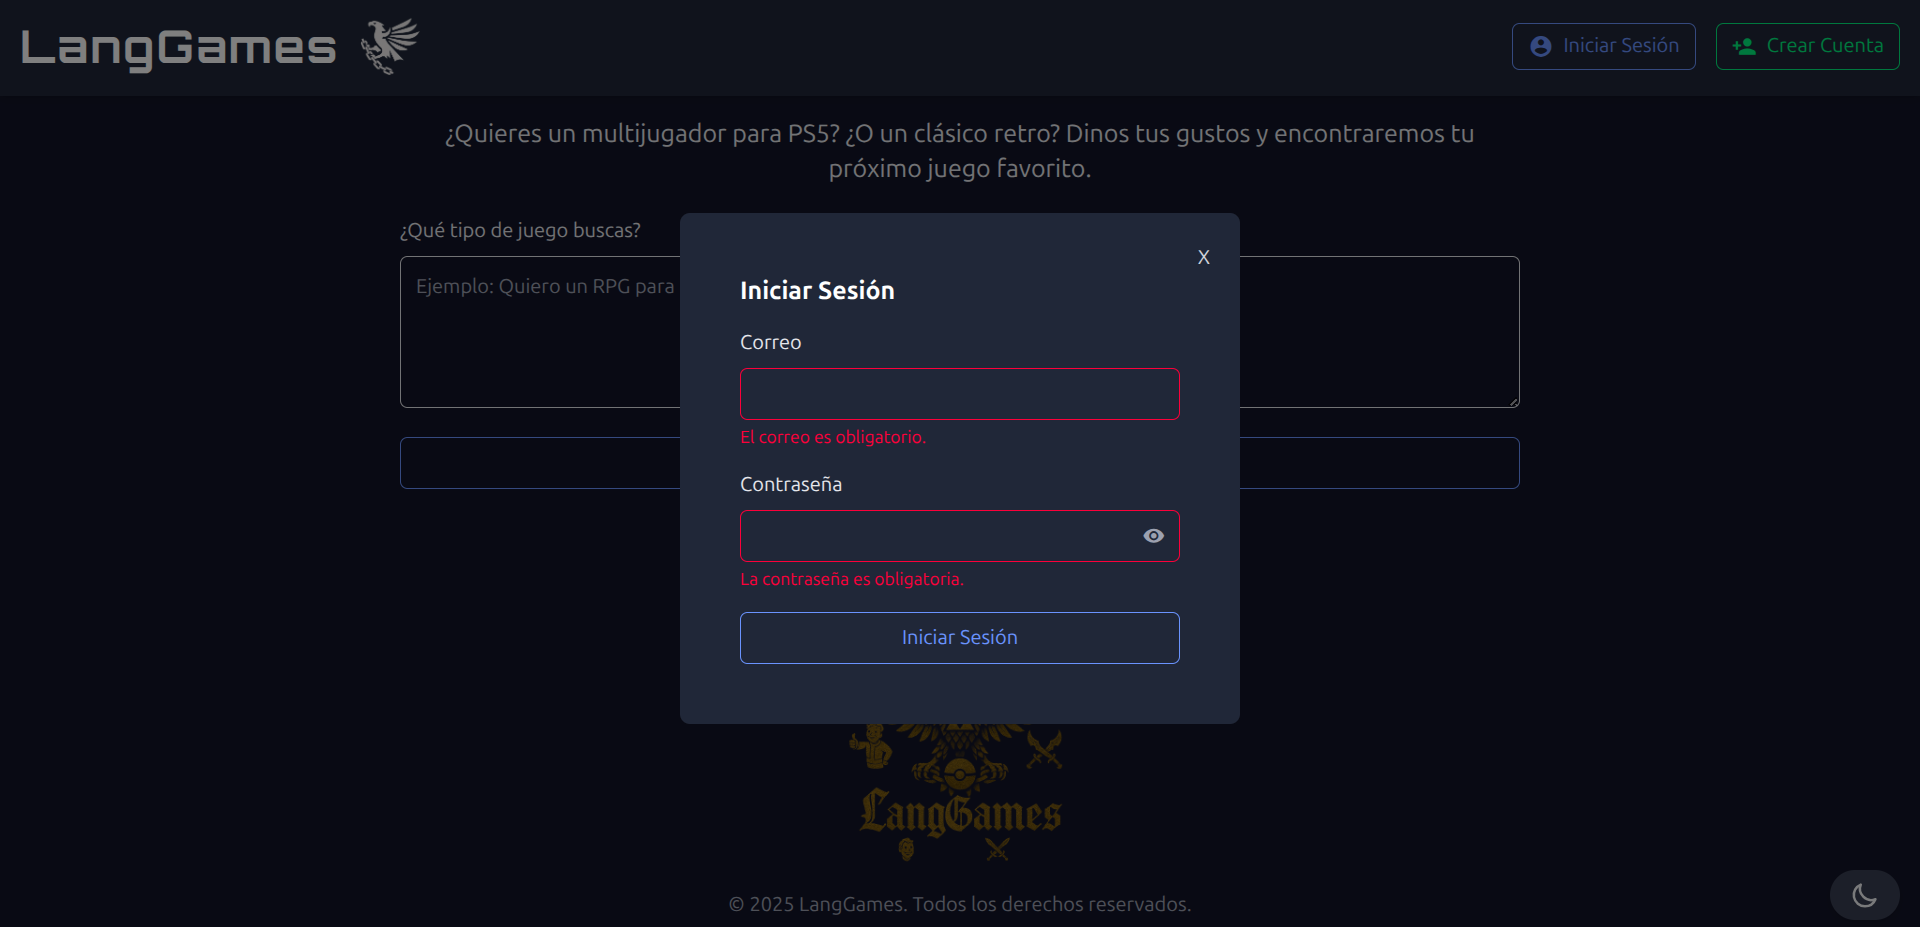
\includegraphics[width=1\linewidth]{imagenes/login.png}
	\caption[\textbf{Inicio de sesión}.]{\textbf{Inicio de sesión}. Formulario para iniciar sesión en la plataforma.}
	\label{imagen-login}
\end{figure}



\subsubsection{Principal}

Este es el componente principal de la aplicación, al que accede el usuario tras iniciar sesión o crear una cuenta.

La interfaz principal incluye una barra superior que muestra el nombre y el logotipo de la plataforma, así como un mensaje de bienvenida personalizado con el nombre del usuario. Además, se incorporan dos botones: uno para acceder a los ajustes de la cuenta y otro para cerrar sesión.

En la parte izquierda de la pantalla se muestran los cuatro próximos lanzamientos. Justo debajo, se encuentran las seis últimas recomendaciones disponibles. En el lateral derecho, hay un cuadro de texto donde el usuario puede solicitar recomendaciones, las cuales se mostrarán en la parte inferior tras ser generadas.

\begin{figure}[H]
	\centering
	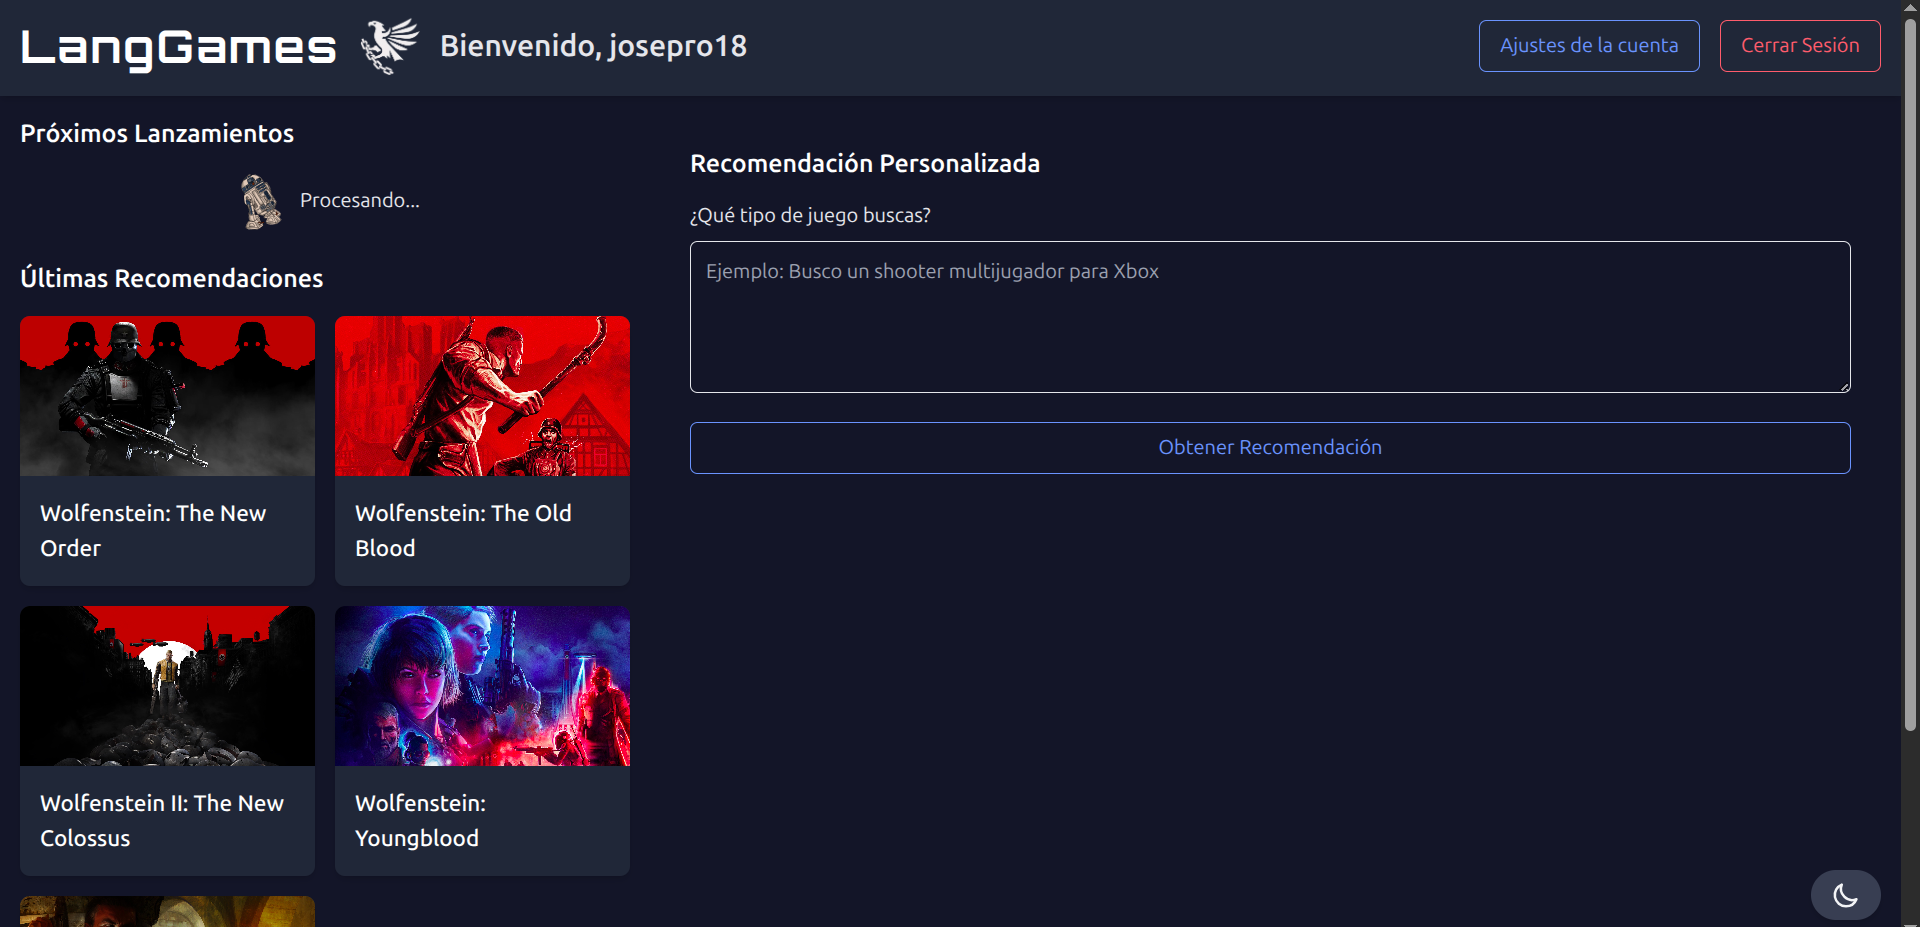
\includegraphics[width=1\linewidth]{imagenes/principal1.png}
	\caption[\textbf{Página principal 1}.]{\textbf{Página principal 1}. Página principal de la plataforma.}
	\label{imagen-principal-1}
\end{figure}

\begin{figure}[H]
	\centering
	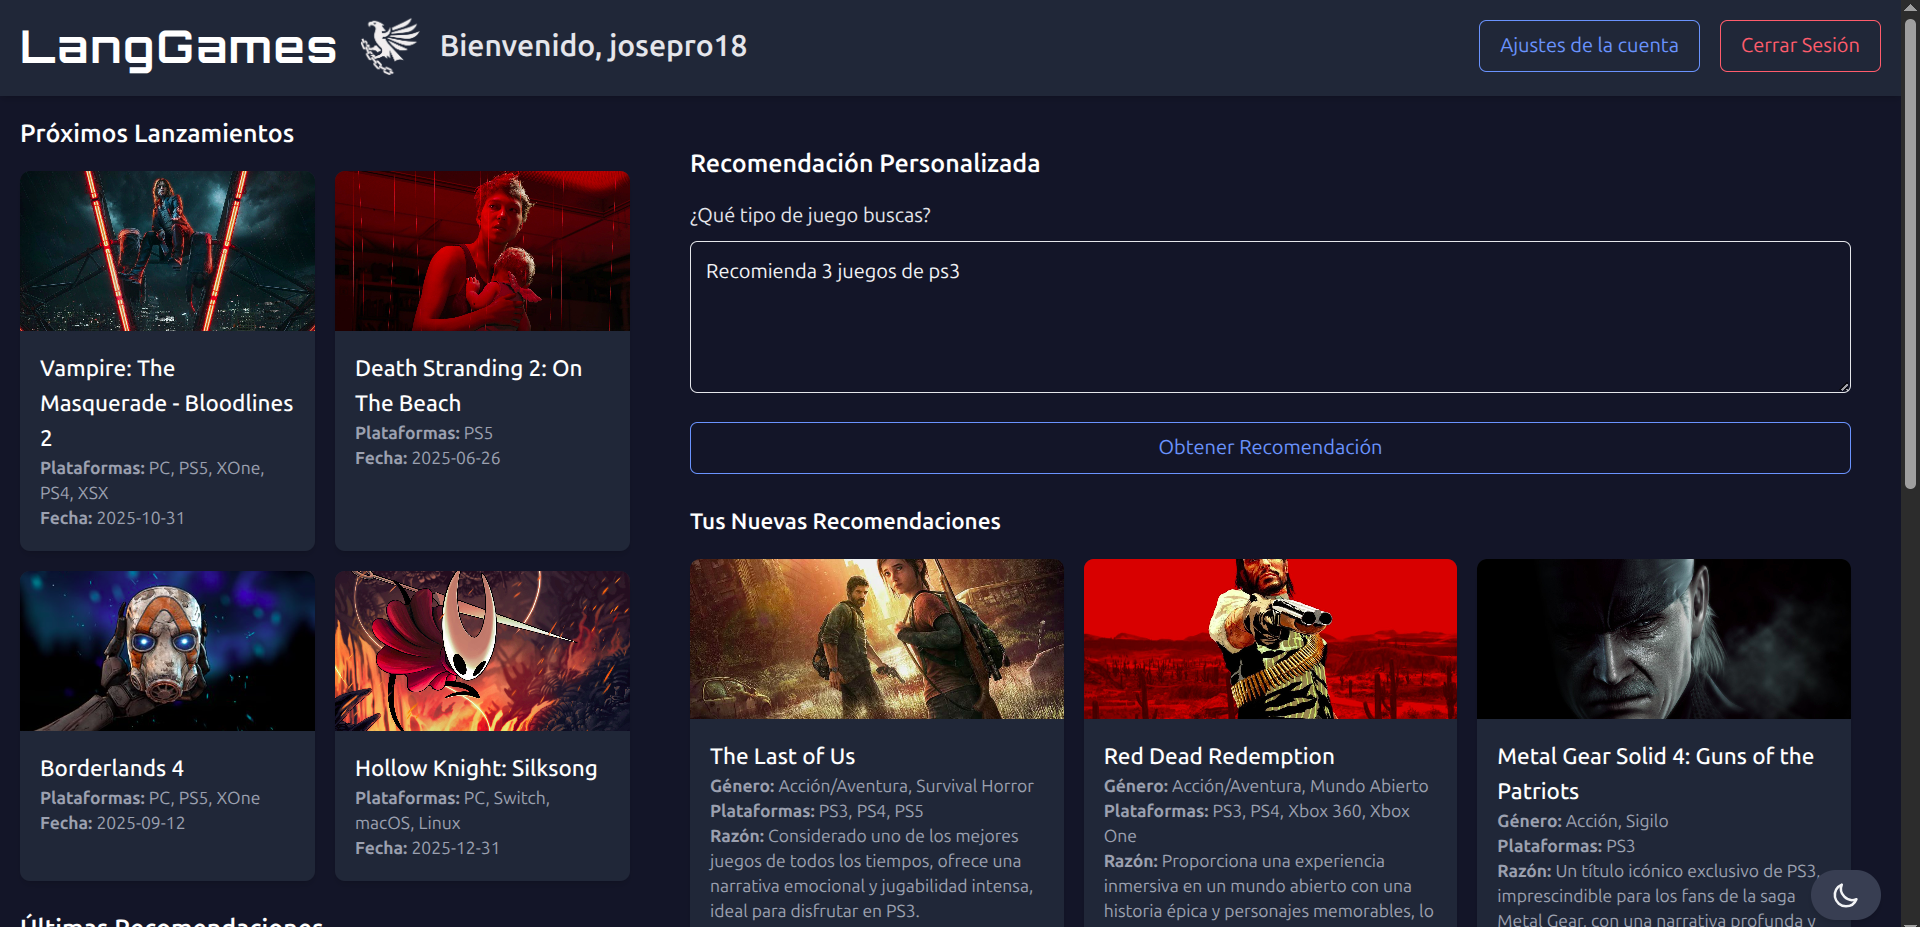
\includegraphics[width=1\linewidth]{imagenes/principal2.png}
	\caption[\textbf{Página principal 2}.]{\textbf{Página principal 2}. Página principal de la plataforma con recomendaciones.}
	\label{imagen-principal-2}
\end{figure}



\subsubsection{Ajustes de cuenta}

La página de ajustes permite al usuario modificar su información personal y gestionar aspectos clave de su cuenta.

En la barra superior se encuentran dos botones: uno para vincular la cuenta con Steam mediante el ID de usuario, y otro para regresar a la página principal.

En la parte izquierda de la página hay otros dos botones. El primero permite cambiar el nombre de usuario y/o la contraseña, o eliminar la cuenta. Para cualquiera de estas acciones, es necesario introducir la contraseña actual. El segundo botón permite restablecer todos los datos relacionados con videojuegos almacenados en la cuenta del usuario. Debajo de estos botones se muestra un resumen con la información sobre los videojuegos del usuario.

En la parte derecha se encuentra un cuadro de texto donde el usuario puede introducir modificaciones mediante lenguaje natural, como por ejemplo indicar la adquisición de una nueva consola o la venta de un juego. El modelo de lenguaje interpreta la petición y aplica la modificación correspondiente, mostrando al usuario un mensaje con el resultado de la operación.

\begin{figure}[H]
	\centering
	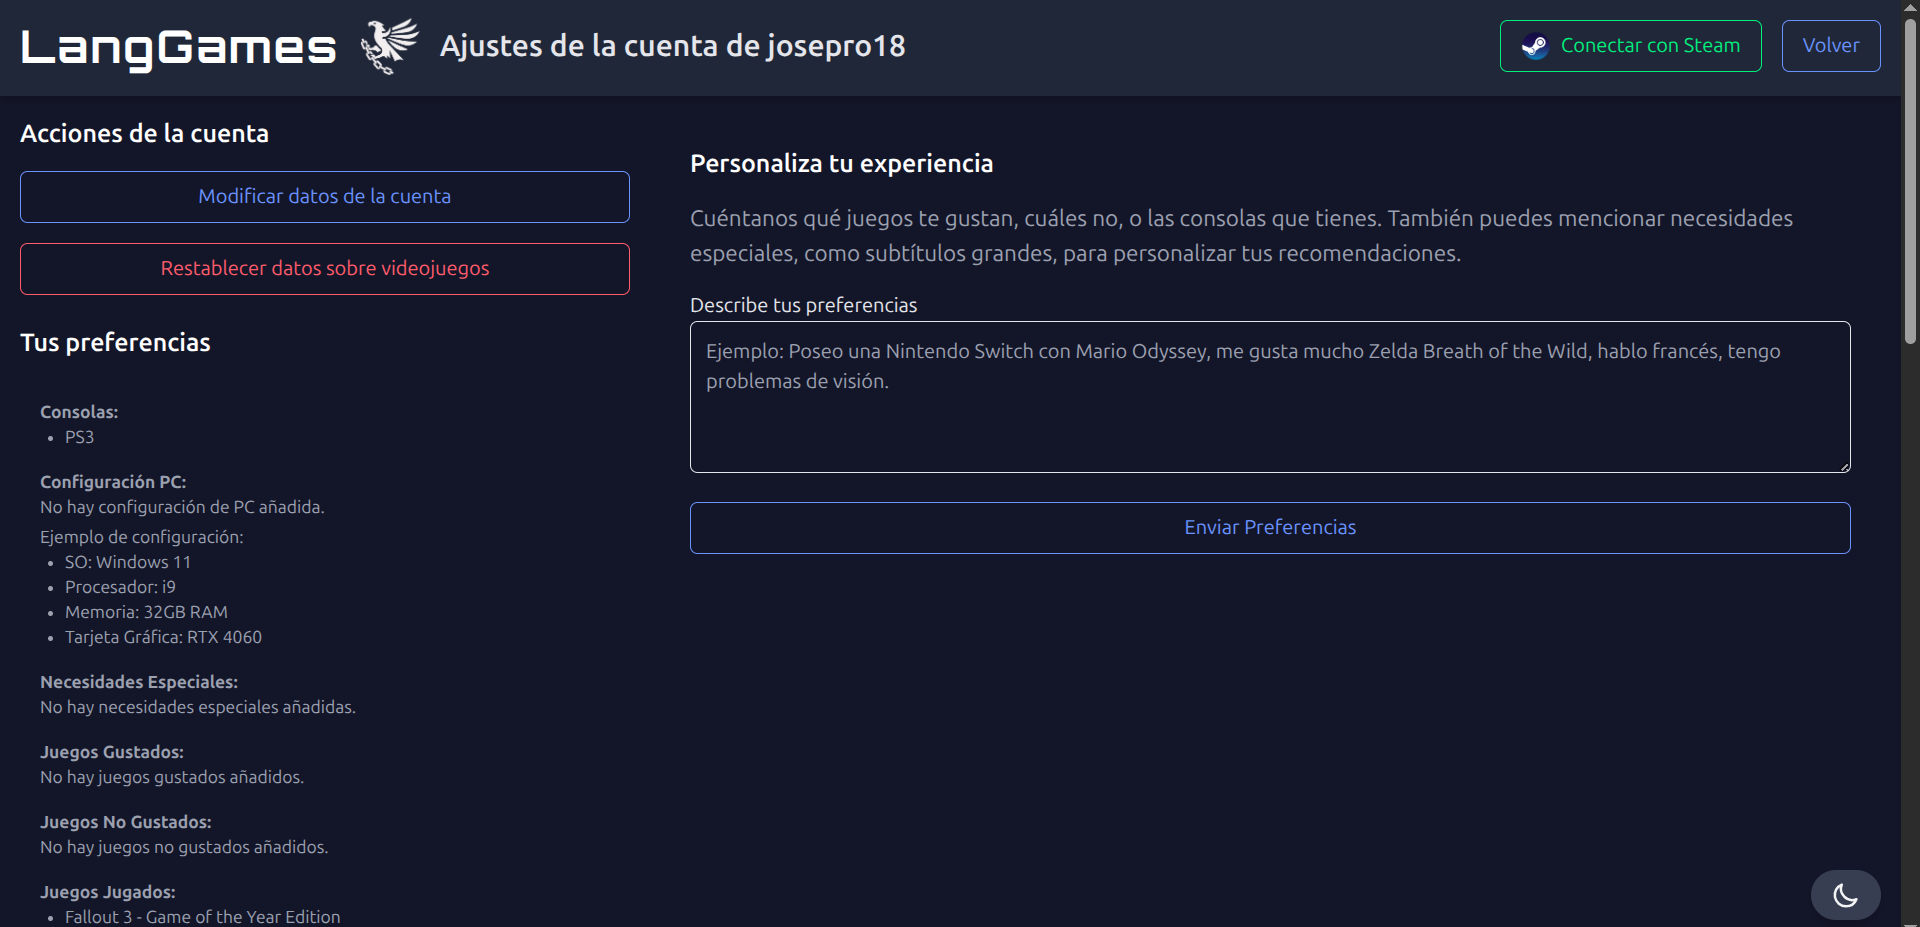
\includegraphics[width=1\linewidth]{imagenes/ajustesCuenta.png}
	\caption[\textbf{Página de ajustes de la cuenta}.]{\textbf{Página de ajustes de la cuenta}. Interfaz donde el usuario puede gestionar la información de su cuenta y realizar ajustes relacionados con sus videojuegos.}
	\label{imagen-ajustes}
\end{figure}

\newpage

\section{Puesta en marcha}

Además, la aplicación incluye tres scripts globales: uno para ejecutar los tres scripts de instalación de los distintos componentes de la plataforma; otro para iniciar el backend y el frontend en segundo plano, almacenando la salida en un archivo de log y guardando sus PIDs para poder detenerlos posteriormente; y un tercer script que permite detener tanto el backend como el frontend que se ejecutan en segundo plano.


\clearpage
\thispagestyle{empty}
\null
\clearpage

\chapter{Pruebas}

En este capítulo, se detallará el proceso de verificación del correcto funcionamiento de la plataforma a través de pruebas unitarias y de integración. 

Describiremos cómo se diseñaron y ejecutaron estas pruebas para garantizar que cada módulo del sistema funcione de manera correcta y que la interacción entre los distintos componentes sea fluida y eficiente. 

Asimismo se abordarán las herramientas y marcos de prueba utilizados, así como los métodos para identificar y corregir posibles errores o inconsistencias. 

Igualmente se discutirán las pruebas de rendimiento, seguridad y usabilidad, evaluando cómo la plataforma responde bajo diferentes condiciones y garantizando una experiencia de usuario óptima.  

\newpage

\section{Pruebas en la \textit{base de datos}}

Para verificar inicialmente el correcto funcionamiento de la base de datos, se utilizó \texttt{mongosh}, la consola interactiva de MongoDB. Se realizaron pruebas básicas para comprobar que el script de instalación creaba correctamente la base de datos y la colección correspondiente.

Además, se llevaron a cabo operaciones de inserción, eliminación y actualización de documentos, evaluando el comportamiento esperado del sistema. A medida que avanzaba el desarrollo del \textit{backend} y el \textit{frontend}, se continuó comprobando que las interacciones con la base de datos se realizaban correctamente, esta vez a través de los métodos implementados en cada uno de estos módulos.

\newpage

\section{Pruebas en el \textit{backend}}

Para realizar pruebas en el \textit{backend}, se utilizó \textbf{Swagger}, una herramienta que permite visualizar y probar de forma interactiva las rutas de una API. Swagger facilita la documentación automática de las APIs RESTful, y en este caso fue generada automáticamente por \texttt{FastAPI}, el framework utilizado para el desarrollo del servidor.

Gracias a Swagger, accesible en la dirección \href{http://localhost:8000/docs\#/}{http://localhost:8000/docs\#/}, se pudieron ejecutar pruebas para cada uno de los endpoints definidos, especificando los campos requeridos, el cuerpo en formato \texttt{JSON} en caso de ser necesario, y visualizando tanto las respuestas del servidor como los posibles errores. Además el propio uvicorn cuando se ejecuta muestra que métodos ejecuta y los errores que ocurren.

Durante el desarrollo, se fue comprobando el correcto funcionamiento de cada uno de los métodos a través de esta interfaz. Esto permitió detectar y corregir errores de manera ágil, gracias a la retroalimentación inmediata proporcionada por la API. Asimismo, se realizaron pruebas introduciendo datos erróneos de forma intencionada con el objetivo de evaluar la robustez del sistema ante entradas inválidas o inconsistentes.

También se simularon escenarios de fallo como la indisponibilidad de los modelos de lenguaje —por ejemplo, debido a un exceso de tokens o a errores en el nombre del modelo— para verificar cómo respondía el sistema en situaciones excepcionales.

Posteriormente, durante el desarrollo del \textit{frontend}, las pruebas comenzaron a realizarse principalmente desde la propia interfaz de usuario. No obstante, en ciertas ocasiones se continuó utilizando Swagger para llevar a cabo pruebas rápidas y directas sobre los endpoints.

\begin{figure}[H]
	\centering
	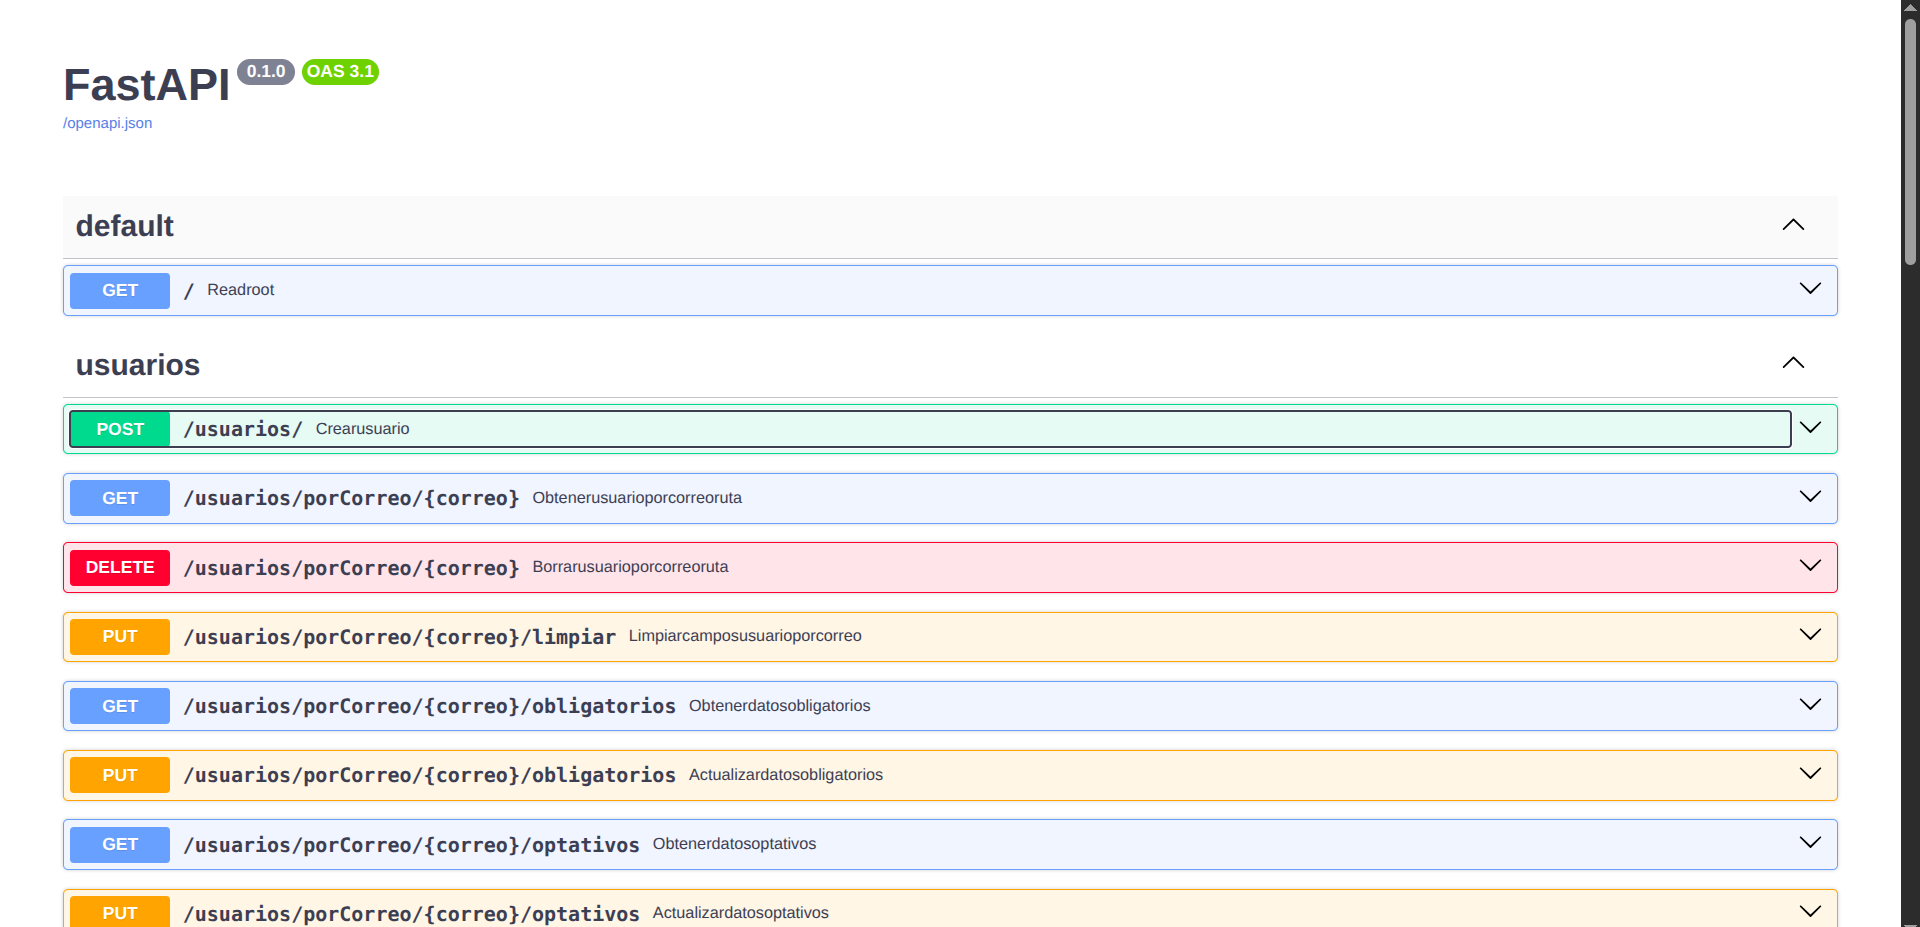
\includegraphics[width=1\linewidth]{imagenes/swagger1.png}
	\caption[\textbf{Vista general de Swagger}.]{\textbf{Vista general de Swagger}. Vista general de la API generada por Swagger a partir del código de FastAPI.}
	\label{swagger-1}
\end{figure}

\begin{figure}[H]
	\centering
	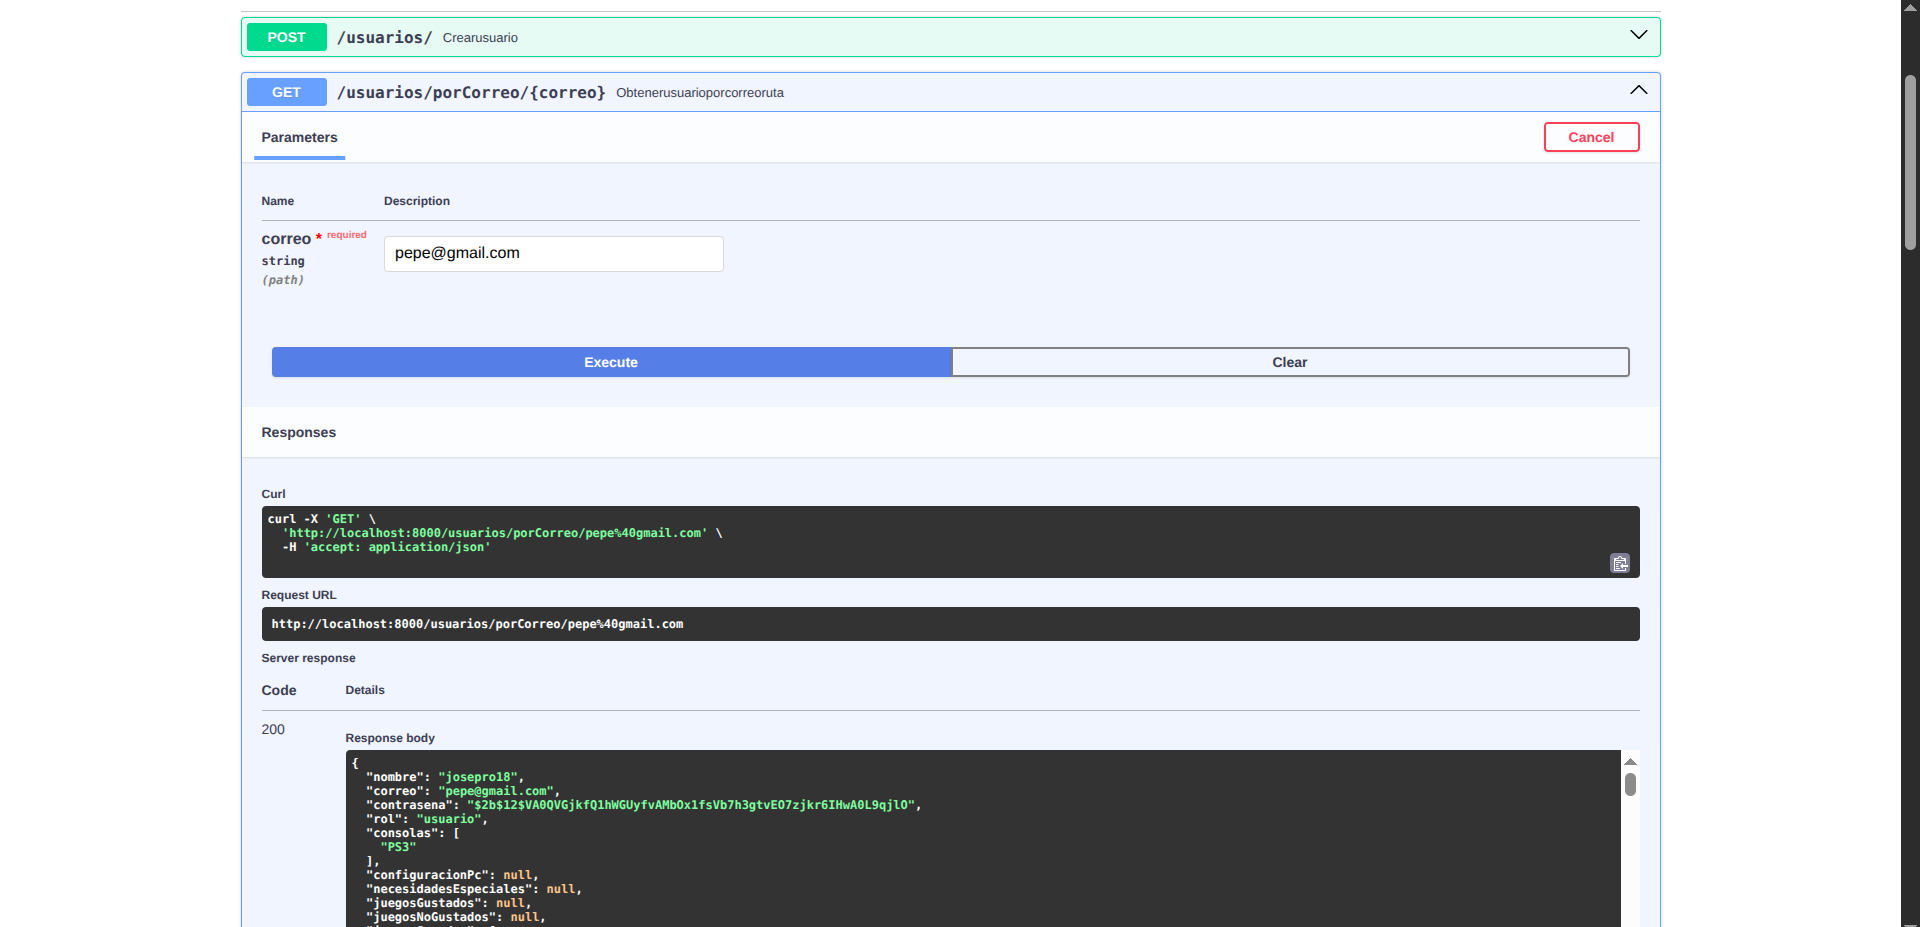
\includegraphics[width=1\linewidth]{imagenes/swagger2.png}
	\caption[\textbf{Vista del uso de un método en Swagger}.]{\textbf{Vista del uso de un método en Swagger}. Se muestra el método \texttt{GET} para obtener un usuario, al que se le pasa el correo electrónico como parámetro, devolviendo un \texttt{JSON} con los datos del usuario.}
	\label{swagger-2}
\end{figure}

\subsection{Pruebas unitarias y de integración en el \textit{backend}}

Además de las pruebas realizadas con Swagger, se han desarrollado pruebas unitarias e integradas para el módulo de \textit{backend} utilizando la librería \texttt{unittest} junto con \texttt{mongomock}, una herramienta que simula el comportamiento de una base de datos MongoDB en memoria. Esto permitió realizar pruebas sin necesidad de conectarse a una base de datos real.

Estas pruebas se organizaron en dos ficheros separados dentro de una carpeta \texttt{test}: un archivo para gestionar usuario y otro para la autentificación. El primero contiene pruebas sobre la lógica de gestión de usuarios, mientras que el segundo verifica las rutas de autenticación expuestas por la API de FastAPI.

Las funciones principales del sistema se comprobaron de forma individual, incluyendo la creación, actualización, eliminación y verificación de usuarios. Para ello, se prepararon entornos simulados en cada prueba, creando una base de datos ficticia e inyectando los datos necesarios para comprobar el comportamiento del sistema. También se emplearon técnicas de \textit{mocking} para simular el comportamiento de las funciones de encriptación de contraseñas (\texttt{bcrypt}) y de generación de tokens JWT, permitiendo centrarse en la lógica del sistema sin depender de funcionalidades externas.

En el caso de las rutas de autenticación, se utilizó \texttt{TestClient}, un cliente de pruebas proporcionado por FastAPI, para simular peticiones HTTP y verificar las respuestas del servidor. Se probaron casos como el inicio de sesión con credenciales correctas, contraseñas incorrectas y usuarios inexistentes, evaluando la respuesta del sistema ante distintos escenarios.

Estas pruebas automáticas permiten garantizar que los métodos clave del \textit{backend} funcionan correctamente, tanto de forma aislada como cuando interactúan entre sí. Además, al ejecutarse de manera repetida, facilitan la detección temprana de errores ante futuros cambios en el código.

\newpage

\section{Pruebas en el \textit{frontend}}

Para llevar a cabo las pruebas en el \textit{frontend}, se inicializó el servidor de Angular y se accedió a la dirección local \href{http://localhost:4200/}{http://localhost:4200/}. Desde esta interfaz se realizaron pruebas interactivas explorando todos los elementos visibles, accionando botones y navegando por los distintos componentes de la aplicación.

La detección de errores se realizaba principalmente a través de dos vías: por un lado, mediante los mensajes devueltos por la API en caso de errores de validación o fallos internos; por otro, mediante el uso de las herramientas de desarrollo del navegador. Estas herramientas, accesibles pulsando \texttt{F12}, permiten inspeccionar múltiples aspectos del comportamiento del sitio web.

En particular, se hizo uso de la \textbf{consola del navegador}, que permite visualizar errores de ejecución de Angular, advertencias, trazas de red, y mensajes de depuración. También se utilizó la pestaña de herramientas de \textit{responsive design}, que simula el comportamiento de la interfaz en diferentes tamaños de pantalla, permitiendo verificar que la aplicación mantiene su usabilidad y legibilidad tanto en dispositivos móviles como en pantallas de escritorio.


\begin{figure}[H]
	\centering
	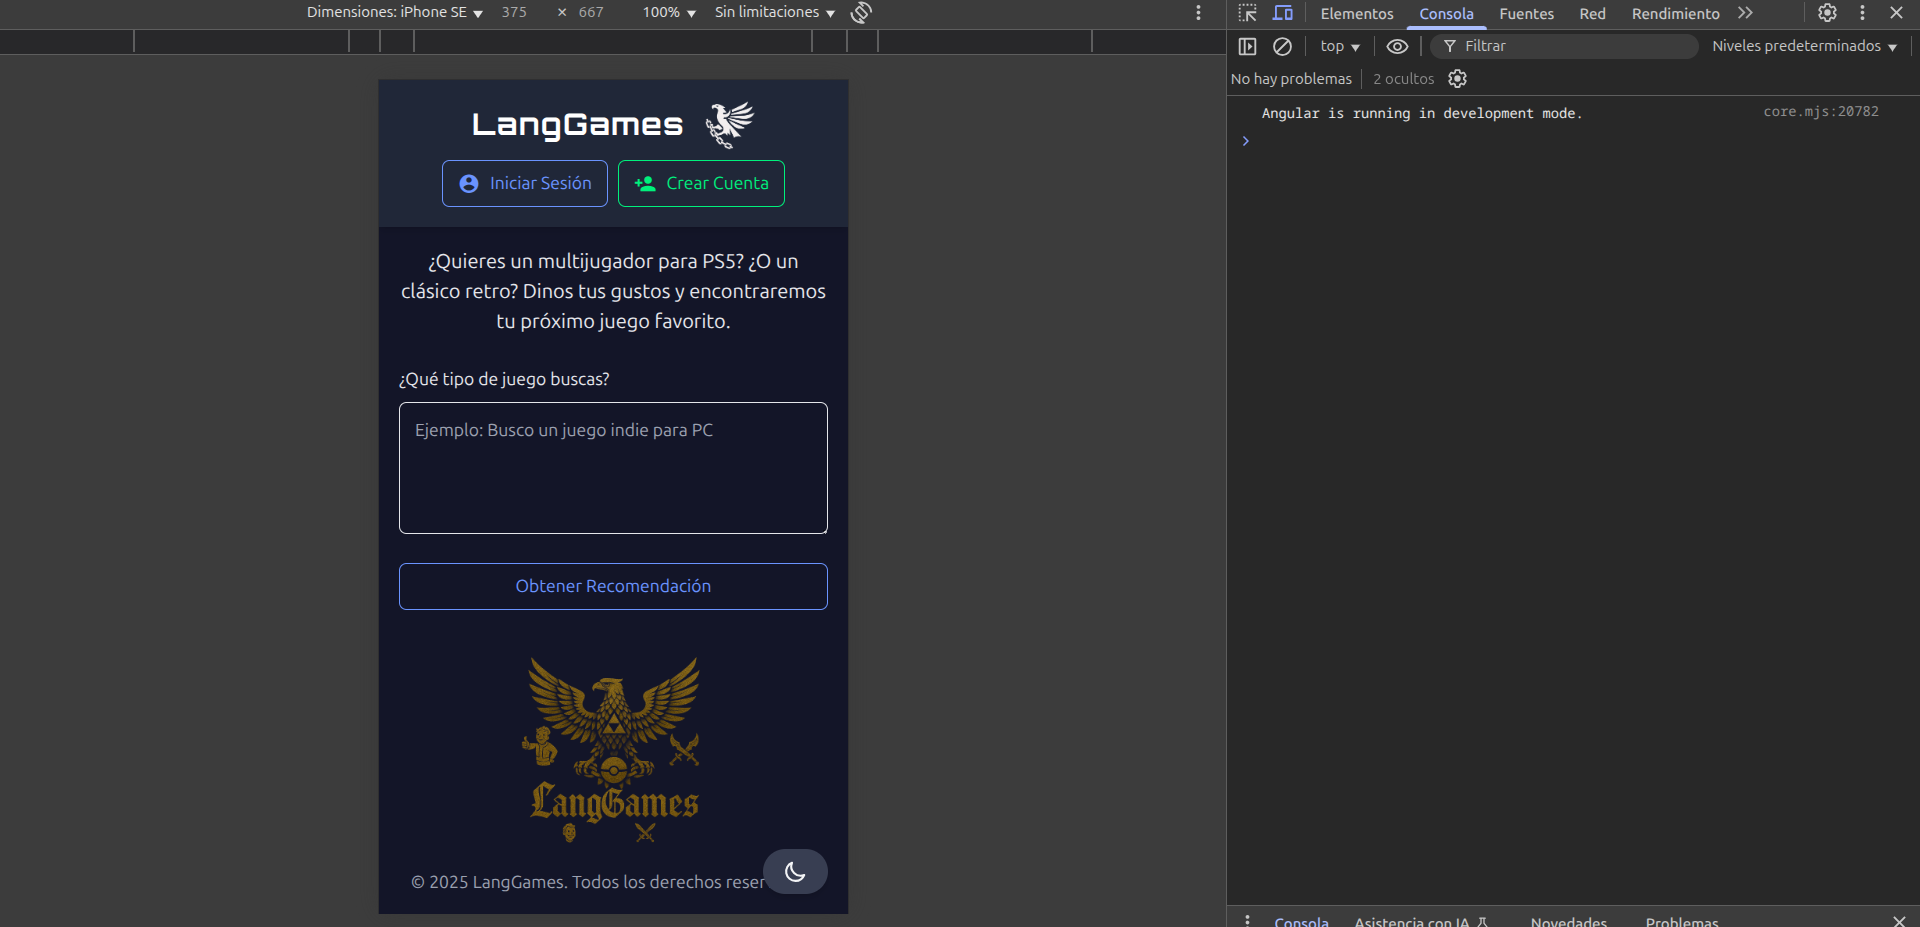
\includegraphics[width=1\linewidth]{imagenes/consolaNavegador.png}
	\caption[\textbf{Vista de las herramientas de desarrollo del navegador}.]{\textbf{Vista de las herramientas de desarrollo del navegador}. Estas herramientas permiten detectar errores de Angular y comprobar que el diseño es adaptable a distintos dispositivos.}
	\label{consola-navegador}
\end{figure}


\subsection{Pruebas unitarias en el \textit{frontend}}

Aunque las pruebas principales del \textit{frontend} se realizaron mediante interacción directa con la aplicación, también se desarrollaron algunas pruebas automáticas para verificar el correcto funcionamiento de ciertos componentes.

Se utilizó el sistema de pruebas de Angular con \texttt{Karma} y \texttt{Jasmine} \cite{green2013angularjs}, configurando un entorno que permite simular peticiones a la API y comprobar que las funciones responden correctamente. En concreto, se probaron aspectos como la gestión de formularios en el componente de inicio de sesión, la validación de campos, el manejo de errores y la navegación tras un inicio de sesión exitoso.

Estas pruebas demostraron ser útiles para asegurar que los servicios y componentes se comportan como se espera. Sin embargo, se decidió no extender su uso al resto de la interfaz, ya que resultaba más efectivo validar el \textit{frontend} desde el punto de vista del usuario, observando directamente cómo se comporta la aplicación en distintos escenarios.


\newpage

\section{Pruebas extras}

Para asegurar una mejor robustez de la plataforma, se ha realizado una instalación de la aplicación en una máquina virtual de Ubuntu nueva, lo que permitió corregir errores que no se vieron durante el desarrollo por instalar las cosas una por una. 

Por ejemplo, la primera vez que se lanza angular se pide al usuario que especifique ciertas preferencias, pero al lanzarse en segundo plano el usuario no podía elegir. Para paliar este problema se realiza un primer lanzamiento de angular en primer plano después de la aplicación.


Además se ha compartido el proyecto con un compañero de informática de la universitat oberta de Catalunya para que pruebe la aplicación y de sus conclusiones. 

\newpage

\section{Conclusión}

A lo largo de este capítulo se ha descrito el proceso de pruebas llevado a cabo para verificar el correcto funcionamiento de cada uno de los módulos de la plataforma.

En primer lugar, se realizaron pruebas directas sobre la base de datos mediante \texttt{mongosh}, asegurando que las operaciones básicas de inserción, actualización y eliminación funcionaban correctamente. Posteriormente, se probó el \textit{backend} utilizando Swagger, lo que permitió evaluar de forma precisa cada uno de los endpoints expuestos por la API, simulando tanto casos correctos como situaciones de error o fallo del sistema.

Finalmente, el \textit{frontend} fue validado mediante interacción directa con la aplicación y mediante el uso de las herramientas de desarrollo del navegador, lo cual permitió no solo identificar errores de ejecución, sino también comprobar la adaptabilidad del diseño a distintos dispositivos.

Este enfoque integral de pruebas, que abarca desde el nivel más bajo (base de datos) hasta el más alto (interfaz de usuario), ha permitido garantizar una plataforma funcional, robusta y preparada para ofrecer una experiencia de usuario óptima. Además, se ha verificado que los distintos componentes interactúan de forma fluida, cumpliendo con los requisitos del sistema.


\clearpage \thispagestyle{empty} \null \clearpage
\chapter{Conclusiones}

Finalmente, en este capítulo debatiremos sobre los resultados obtenidos a lo largo del proyecto. Reflexionaremos sobre el cumplimiento de los objetivos planteados al inicio y evaluaremos la efectividad de las soluciones implementadas. 

Además, se analizarán los puntos fuertes y las limitaciones de la plataforma desarrollada, así como las posibles áreas de mejora. 


Del mismo modo se considerarán las implicaciones de los resultados obtenidos en el contexto de la industria de los videojuegos. 


Por último, se propondrán futuras líneas de trabajo que podrían extenderse a otras áreas, basándose en los resultados y conocimientos adquiridos.  

\newpage

\section{Conclusiones de la aplicación}

A lo largo de este proyecto se ha puesto de manifiesto la relevancia actual tanto del sector de los videojuegos como de los modelos de lenguaje natural. La creciente importancia de ambos campos genera nuevas oportunidades para desarrollar aplicaciones que ayuden a gestionar, explorar y conectar los elementos que los componen.

En este contexto, herramientas como \textbf{LangChain} y \textbf{OpenRouter} han demostrado ser especialmente potentes a la hora de integrar diferentes modelos de lenguaje de manera flexible. Gracias a ellas, es posible aprovechar el potencial de la inteligencia artificial de forma accesible, facilitando el desarrollo de nuevas soluciones o la mejora de sistemas existentes mediante funcionalidades basadas en lenguaje natural.

La plataforma desarrollada, \textbf{LangGames}, representa un primer paso hacia una solución que facilite al usuario la elección de un videojuego entre la inmensa oferta actual. La idea es ofrecer un sistema de recomendación sencillo e intuitivo, que funcione a partir de una breve descripción en lenguaje natural, y que además pueda mejorar progresivamente gracias a la información acumulada y al razonamiento de los procesadores de lenguaje subyacentes.

En términos generales, se puede afirmar que la mayoría de los objetivos planteados han sido alcanzados. La aplicación es capaz de recomendar videojuegos en base a preferencias expresadas por los usuarios, presenta una interfaz visualmente atractiva y ha demostrado un comportamiento robusto y razonablemente eficiente.

No obstante, durante el desarrollo surgieron ciertos obstáculos que motivaron cambios en el planteamiento inicial. Por ejemplo, no se implementó un sistema completo de usuarios administradores, ya que muchas de sus funcionalidades pudieron gestionarse directamente desde las herramientas de desarrollo. Del mismo modo, las restricciones de uso en OpenRouter, especialmente en cuanto al número de tokens disponibles, limitaron el alcance de las pruebas y la variedad de modelos evaluados.

Otro aspecto a mejorar es el tiempo de respuesta de los modelos, que resulta elevado debido al uso de una API externa y gratuita. Aunque es una limitación comprensible, puede afectar negativamente a la experiencia de usuario. Asimismo, las medidas de seguridad implementadas son limitadas, debido tanto al desconocimiento previo como a problemas técnicos encontrados al intentar añadir capas de seguridad más avanzadas.

Además, la falta de recursos económicos ha impedido realizar un despliegue en la web, lo cual habría sido ideal para validar la plataforma con usuarios reales y analizar su impacto.

Con un presupuesto adecuado, esta aplicación podría evolucionar hasta convertirse en una herramienta esencial para jugadores habituales. La incorporación de modelos más avanzados, con capacidad de búsqueda en internet precisa y una mejor integración con plataformas de videojuegos como las de Microsoft o Sony, podría situar a LangGames dentro del ecosistema digital de los videojuegos modernos.

Más allá de los videojuegos, este tipo de tecnología tiene un gran potencial de extrapolación a otros medios culturales como el cine, las series, la literatura o la música. Gracias a su flexibilidad y capacidad de comprensión del lenguaje, los modelos de IA seguirán expandiéndose y ganando protagonismo en múltiples ámbitos de la vida cotidiana. Los modelos de lenguaje han llegado para quedarse, y su papel será cada vez más central en el desarrollo de nuevas herramientas y servicios inteligentes.

\newpage

\section{Conclusiones personales}

A pesar de las dificultades personales que han acompañado el desarrollo de este trabajo, la valoración final es personalmente positiva.

Ha sido muy gratificante comprobar cómo una idea inicial, casi esbozada, ha ido tomando forma paso a paso hasta convertirse en una aplicación funcional. Como persona que ha consumido videojuegos durante toda su vida, ha sido una experiencia transformadora pasar del rol de usuario al de creador, desarrollando una utilidad que potencialmente podría ser utilizada por miles de personas con los mismos intereses.

Además, este trabajo ha servido como una muestra del progreso alcanzado a lo largo del grado. Desde los primeros pasos con programas muy básicos hasta la creación de una aplicación completa desde 0, integrando tecnologías como \textit{FastAPI}, \textit{LangChain}, \textit{MongoDB} y \textit{Angular}, queda patente la evolución tanto técnica como personal.

El proceso también ha fomentado el desarrollo de habilidades de investigación y aprendizaje autodidacta. Por ejemplo, se ha pasado de tener una comprensión superficial de lo que era una API, a diseñar e implementar una propia, completamente funcional y conectada con una base de datos y una interfaz web.

Aunque el proyecto pueda parecer sencillo o limitado desde una perspectiva externa, lo cierto es que implica un esfuerzo considerable, muchas horas de dedicación y una gran cantidad de conocimientos adquiridos y aplicados. Más allá del resultado final, lo que realmente queda es una sensación de logro y una base sólida sobre la que seguir construyendo en el futuro.5


\clearpage \thispagestyle{empty} \null \clearpage

% Bibliografía
\cleardoublepage
\phantomsection
\addcontentsline{toc}{chapter}{Bibliografía}
\printbibliography
\clearpage \thispagestyle{empty} \null \clearpage
\end{document}